\documentclass[12pt,a4paper]{article}
\usepackage[utf8]{inputenc}
\usepackage{ctex}
\usepackage[margin=2.5cm]{geometry}
\usepackage{amsmath,amssymb,amsfonts}
\usepackage{graphicx}
\usepackage{float}
\usepackage{booktabs}
\usepackage{natbib}
\usepackage{fancyhdr}
\usepackage{titlesec}
\usepackage{xcolor}
\usepackage{hyperref}
% 添加算法相关包
\usepackage[ruled,vlined]{algorithm2e}
\usepackage{algorithmic}
\usepackage{caption}
\usepackage{subcaption}  % 放在导言区,替代旧的 subfigure 宏包
% 其他可能需要的包
\usepackage{geometry}
\usepackage{setspace}
% 在文档导言区添加
\usepackage{array}
\usepackage{algorithm2e}
% 设置页眉页脚
\pagestyle{fancy}
\fancyhf{}
\setlength{\headheight}{15pt}
\fancyhead[C]{\textit{Research Report on Handwritten Digit Recognition}}
\fancyfoot[C]{\thepage}
\renewcommand{\headrulewidth}{0.5pt}

% 设置标题格式 - 更简洁的样式
\titleformat{\section}
{\Large\bfseries}{\thesection}{1em}{}
\titleformat{\subsection}
{\large\bfseries}{\thesubsection}{1em}{}

% 设置超链接样式
\hypersetup{
    colorlinks=true,
    linkcolor=black,
    citecolor=black,
    urlcolor=blue
}

\begin{document}

\begin{titlepage}
    \centering
    \vspace*{2.5cm}

    % 中文标题
    {\LARGE\bfseries 手写数字识别研究报告 \par}
    \vspace{0.8cm}
    % 英文副标题
    {\large\itshape Research Report on Handwritten Digit Recognition \par}

    \vspace{2.5cm}

    % 作者信息(五人居中对齐)
    \begin{center}
    \begin{tabular}{ccc}
        \textbf{张三} & \textbf{李四} & \textbf{王五} \\
        北京邮电大学 & 北京邮电大学 & 北京邮电大学 \\
        zhangsan@univ.edu.cn & lisi@univ.edu.cn & wangwu@univ.edu.cn \\
    \end{tabular}

    \vspace{1.2cm}

    \begin{tabular}{cc}
        \textbf{赵六} & \textbf{孙七} \\
        北京邮电大学 & 北京邮电大学 \\
        zhaoliu@univ.edu.cn & sunqi@univ.edu.cn \\
    \end{tabular}
    \end{center}

    \vfill

    {\normalsize\today\par}
\end{titlepage}


% 添加简洁的分割线
\newcommand{\sectionline}{%
    \noindent\makebox[\linewidth]{\rule{0.8\paperwidth}{0.4pt}}
}

% 摘要页
\newpage
\begin{abstract}
本论文以手写数字识别这一人工智能领域的基础实验为支点,探索了全连接神经网络(MLP),卷积神经网络(CNN)基本原理以及在图像分类领域的应用。
通过变更MLP隐层神经元数量,并降维可视化了训练过程中特征空间的点簇聚类效果,揭示了隐层神经元意义与神经网络的聚类能力。
同时,我们将神经网络抽象为特征提取器和分类器的组合,通过分别冻结特征提取器的权重与分类器的权重,深刻揭示了神经网络的特征提取能力。
在CNN的实验中,我们着重关注了对特征图的可视化,深化了对卷积操作的理解。
我们还对神经网络的作用机理进行了猜测,试验了神经网络在未观测数据模式下的表现。



\
\textbf{关键词:} 手写数字识别;全连接神经网络;卷积神经网络;特征提取;图像分类
\end{abstract}

\sectionline

\newpage
\tableofcontents

\newpage

\section{引言}
手写数字识别作为模式识别领域的基础任务之一,长期以来在人工智能、图像处理和神经计算等研究中占据着重要地位。尽管其任务形式相对简单,但却为我们理解神经网络的工作机制提供了理想平台。随着深度学习的发展,从传统的多层感知机(MLP)到现代的卷积神经网络(CNN),模型结构不断演化,对图像分类任务的建模能力也在持续提升 \cite{lecun1998gradient, krizhevsky2012imagenet}。

本研究以 MNIST 数据集为实验对象,旨在通过逐层剖析神经网络的结构和行为,深入理解其特征提取与分类能力。我们不仅复现了经典的全连接网络训练过程,还进一步通过改变隐层神经元数量、冻结部分参数、观察训练动态等方式,从多个角度分析了神经网络“学习”的本质。最后,通过卷积网络中的特征图可视化实验,我们更直观地理解了网络中间层的语义表示过程。


\section{相关工作}

手写数字识别最早的经典方法可以追溯到支持向量机(SVM)、K 近邻(KNN)等浅层模型 \cite{cortes1995support, alpaydin2004introduction}。但随着深度神经网络的发展,LeCun 等人提出的 LeNet-5 卷积神经网络在 MNIST 上取得了划时代的性能表现 \cite{lecun1998gradient},成为后续深度学习研究的重要基准。

近年来,大量研究致力于分析深度神经网络的可解释性与结构可视化。如 Zeiler 和 Fergus 提出的反卷积可视化方法 \cite{zeiler2014visualizing},帮助我们理解 CNN 不同层提取的图像特征;t-SNE 降维方法 \cite{maaten2008visualizing} 也被广泛用于展示中间层特征的聚类能力。

此外,近年来也有部分工作关注神经网络模块化结构,如将网络分解为特征提取器与分类器两部分进行独立分析 \cite{yosinski2014transferable}。这些研究表明,特征提取器往往承担了更重要的学习任务,而分类器部分则可以通过少量微调快速适应新任务。

本研究在上述工作的基础上,进一步引入“参数冻结”等操作,系统性分析特征提取器与分类器的作用机制,并结合中间层特征图可视化,构建出一套完整的实验体系用于理解神经网络的内部行为。

\textbf{项目源代码:}\url{https://github.com/ZZL-2005/Mnist}
\section{手写数字识别数据集(MNIST)}
MNIST(Modified National Institute of Standards and Technology)是一个经典的手写数字图像数据集,由 LeCun 等人在 1998 年整理并公开发布,用于评估图像分类算法的性能 \cite{lecun1998gradient}。数据集包含来自 0 至 9 的共 10 类手写数字图像,每张为 $28 \times 28$ 的灰度图像,其中训练集共 60,000 张,测试集为 10,000 张。由于其标注准确、处理规范,MNIST 常被视为图像识别领域的入门级基准数据集。
我们对数据集的部分统计特征执行了可视化
\begin{figure}[H]
    \centering
    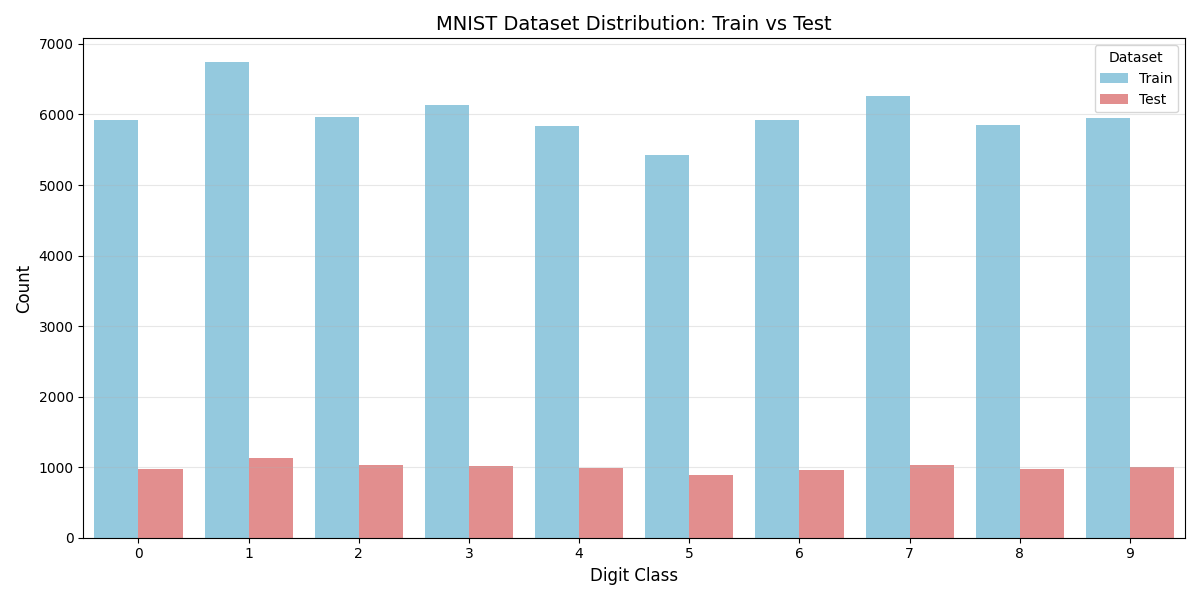
\includegraphics[width=0.8\textwidth]{../images/bqfb.png}
    \caption{标签分布}
    \label{fig:td}
\end{figure}
\begin{figure}[h]
    \centering
    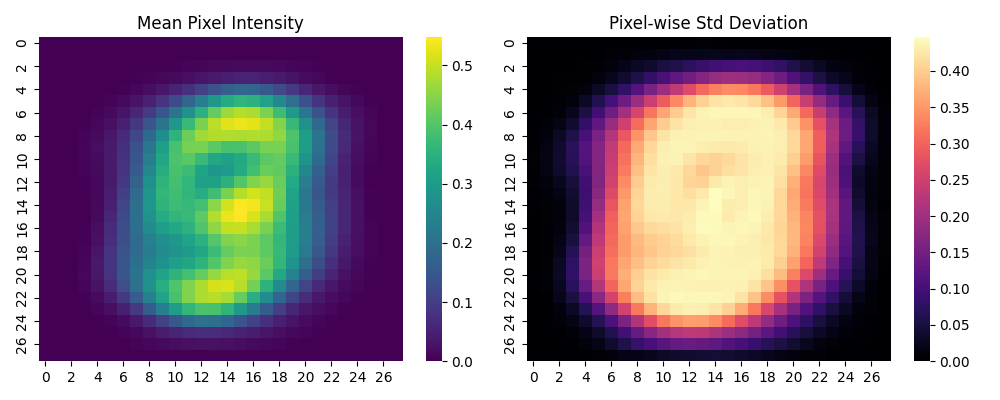
\includegraphics[width=0.8\textwidth]{../images/xsfb.png}
    \caption{像素分布}
    \label{fig:xd}
\end{figure}
图\ref{fig:td}展示了MNIST数据集中各个数字的标签分布情况,可以看出每个数字的样本数量大致相同,表明数据集是均衡的。图\ref{fig:xd}则展示了所有图像中像素值统计特征。
像素值特征统计之前,所有像素都被归一化到 $[0, 1]$ 区间。左图统计了每个位置的像素均值,右图统计了每个位置的像素标准差。可以看到,数据集所代表的都是典型的手写数字图像,集中于图像中央,不存在大量的偏离中央的数据。
在我们的后续实验中,为了提高训练效率,节约算力资源,我们在不影响实验结果的前提下对数据集进行了裁剪,只取一部分数据作为我们的数据集\ref{fig:sssss}。
\begin{figure}[h]
    \centering
    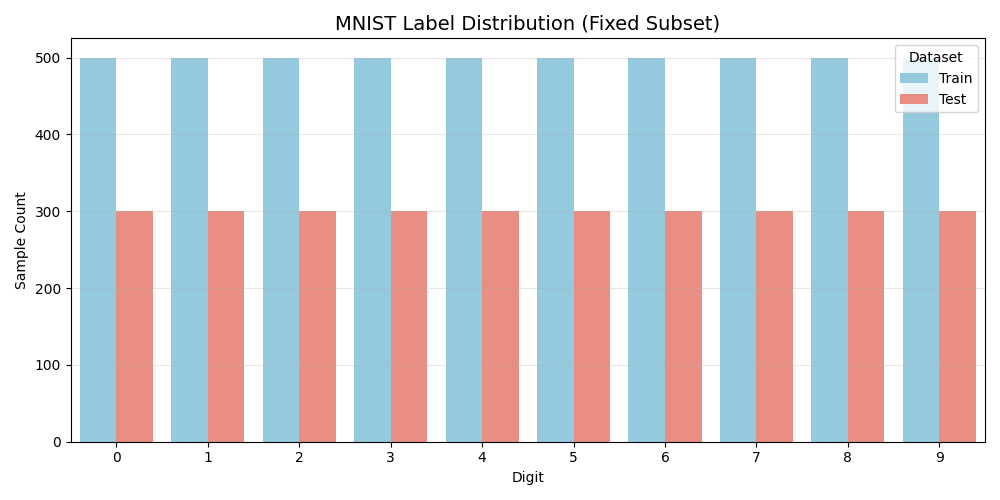
\includegraphics[width=0.8\textwidth]{../images/zjfb.png}
    \caption{子集分布}
    \label{fig:sssss}
\end{figure}
\section{全连接神经网络}
多层感知机(Multilayer Perceptron, MLP)是最早被提出且广泛应用的神经网络结构之一,其核心特点是各层之间全连接,并通过非线性激活函数实现对复杂函数的拟合能力。尽管感知机模型最早由 Rosenblatt 于 1958 年提出 \cite{Rosenblatt1958},但由于单层感知机只能处理线性可分问题,该模型在20世纪70年代一度受到质疑。直到 1986 年,Rumelhart、Hinton 与 Williams 提出了反向传播(Backpropagation)算法 \cite{Rumelhart1986},使得多层感知机可以高效训练,显著增强了其非线性建模能力,推动神经网络进入新的发展阶段。
我们下面所讨论的神经网络都是基于反向传播算法的。
\subsection{模型架构}
\begin{figure}[H]
    \centering
    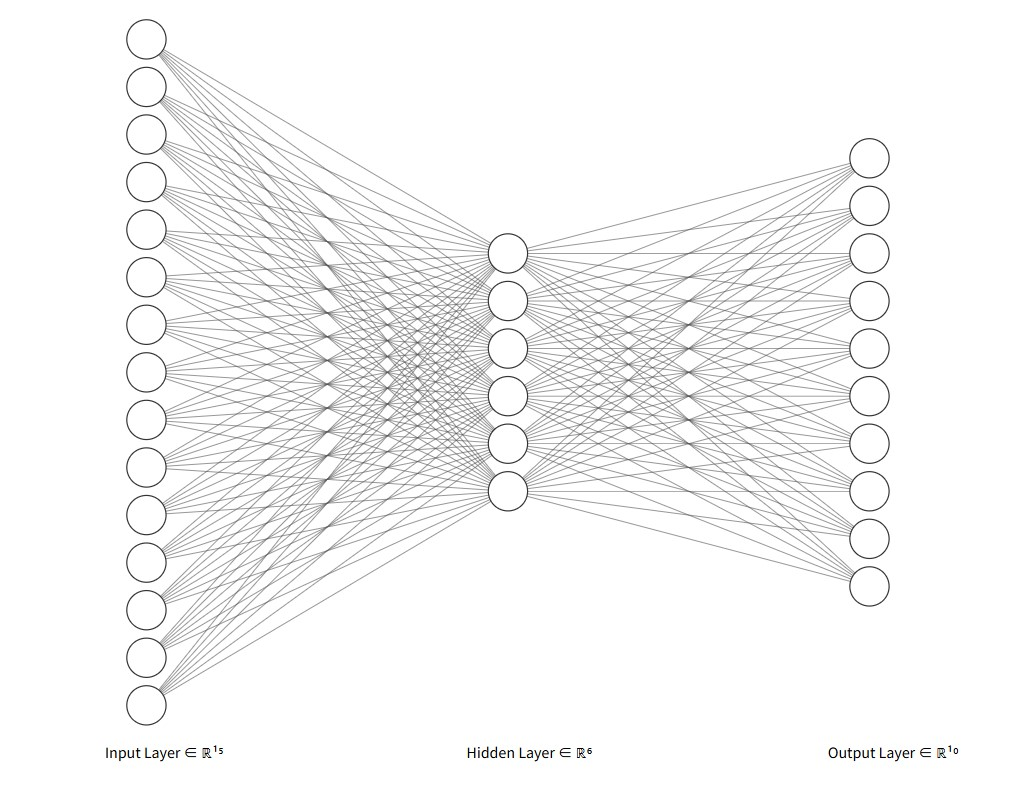
\includegraphics[width=0.8\textwidth]{../images/1.jpg}
    \caption{MLP结构图}
    \label{fig:mlpstructure}
\end{figure}
参考图\ref{fig:mlpstructure},全连接神经网络是一个层级结构,每一层有多个神经元,且每一个神经元都对前一层和后一层的所有神经元实现全连接。
每一条连接都有一个权重参数,一个神经元的输入是前一层所有神经元的输出的加权和再加上一个偏置项,输出则是输入经过激活函数处理后的结果。
最后一层神经元的数目代表了分类的类别数,输出结果经过softmax函数执行归一化处理后,得到每个类别的概率分布。权重与偏置都基于梯度优化算法,梯度的计算通过反向传播算法实现。关于模型和反向传播算法更加详细的介绍,请参考附录\ref{sec:mlpbp}。


\begin{algorithm}[H]
\SetAlgoLined
\KwData{训练数据集 $\{(x^{(i)}, y^{(i)})\}_{i=1}^{m}$,学习率 $\alpha$,网络权重 $W^{(l)}$,偏置 $b^{(l)}$}
\KwResult{优化后的网络参数}

\textbf{初始化:}随机初始化所有权重和偏置\;

\For{每个训练轮次}{
    \For{每个训练样本 $(x^{(i)}, y^{(i)})$}{
        \textbf{前向传播:}\;
        $a^{(0)} = x^{(i)}$\;
        \For{$l = 1$ \KwTo $L$}{
            $z^{(l)} = W^{(l)} a^{(l-1)} + b^{(l)}$\;
            $a^{(l)} = \sigma(z^{(l)})$\;
        }
        
        \textbf{计算输出层误差:}\;
        $\delta^{(L)} = \nabla_a C \odot \sigma'(z^{(L)})$\;
        
        \textbf{反向传播误差:}\;
        \For{$l = L-1$ \KwTo $1$}{
            $\delta^{(l)} = ((W^{(l+1)})^T \delta^{(l+1)}) \odot \sigma'(z^{(l)})$\;
        }
        
        \textbf{计算梯度:}\;
        \For{$l = 1$ \KwTo $L$}{
            $\frac{\partial C}{\partial W^{(l)}} = \delta^{(l)} (a^{(l-1)})^T$\;
            $\frac{\partial C}{\partial b^{(l)}} = \delta^{(l)}$\;
        }
        
        \textbf{更新参数:}\;
        \For{$l = 1$ \KwTo $L$}{
            $W^{(l)} = W^{(l)} - \alpha \frac{\partial C}{\partial W^{(l)}}$\;
            $b^{(l)} = b^{(l)} - \alpha \frac{\partial C}{\partial b^{(l)}}$\;
        }
    }
}

\caption{多层感知机反向传播算法}
\label{alg:mlp_backprop}
\end{algorithm}
\subsection{实验一:简单反向传播的实现}
\subsubsection{实验设置}
本实验中,我们手动实现了一个仅含一个隐藏层的MLP模型,以及MLP模型上的BP算法。
该实现不依赖任何深度学习框架的自动求导机制,而是通过手动计算梯度并执行参数更新,完成完整的反向传播训练流程。模型结构包括一个隐藏层,激活函数采用 ReLU,输出层使用 Softmax 并以交叉熵作为损失函数。
\begin{table}[H]
\centering
\caption{手动实现的MLP实验参数设置}
\label{tab:manual_mlp_config}
\begin{tabular}{ll}
\toprule
\textbf{参数名称} & \textbf{取值 / 描述} \\
\midrule
输入维度(Input Dimension) & 784($28 \times 28$ 图像展平) \\
隐藏层神经元数(Hidden Units) & 30 \\
输出维度(Output Classes) & 10 类(数字 0--9) \\
激活函数(Activation Function) & ReLU(隐藏层) + Softmax(输出层) \\
损失函数(Loss Function) & 多类交叉熵损失(Cross Entropy) \\
学习率(Learning Rate) & 0.01 \\
批量大小(Batch Size) & 256 \\
训练轮数(Epochs) & 80 \\
优化方式(Optimizer) & 小批量梯度下降(Mini-batch Gradient Descent) \\
数据集来源 & MNIST 子集(每类训练样本 500,测试样本 300) \\
参数初始化方式 & He 初始化(适用于 ReLU) \\
日志记录 & 记录每轮准确率、损失、时间,保存为 JSON \\
输出图像 & 训练曲线、混淆矩阵(保存为 PNG) \\
\bottomrule
\end{tabular}
\end{table}
\subsubsection{结果分析}
为分析训练过程,我们记录了每轮训练的准确率与损失,并保存了训练日志与可视化结果,包括训练曲线和混淆矩阵。
\begin{figure}[H]
    \centering
    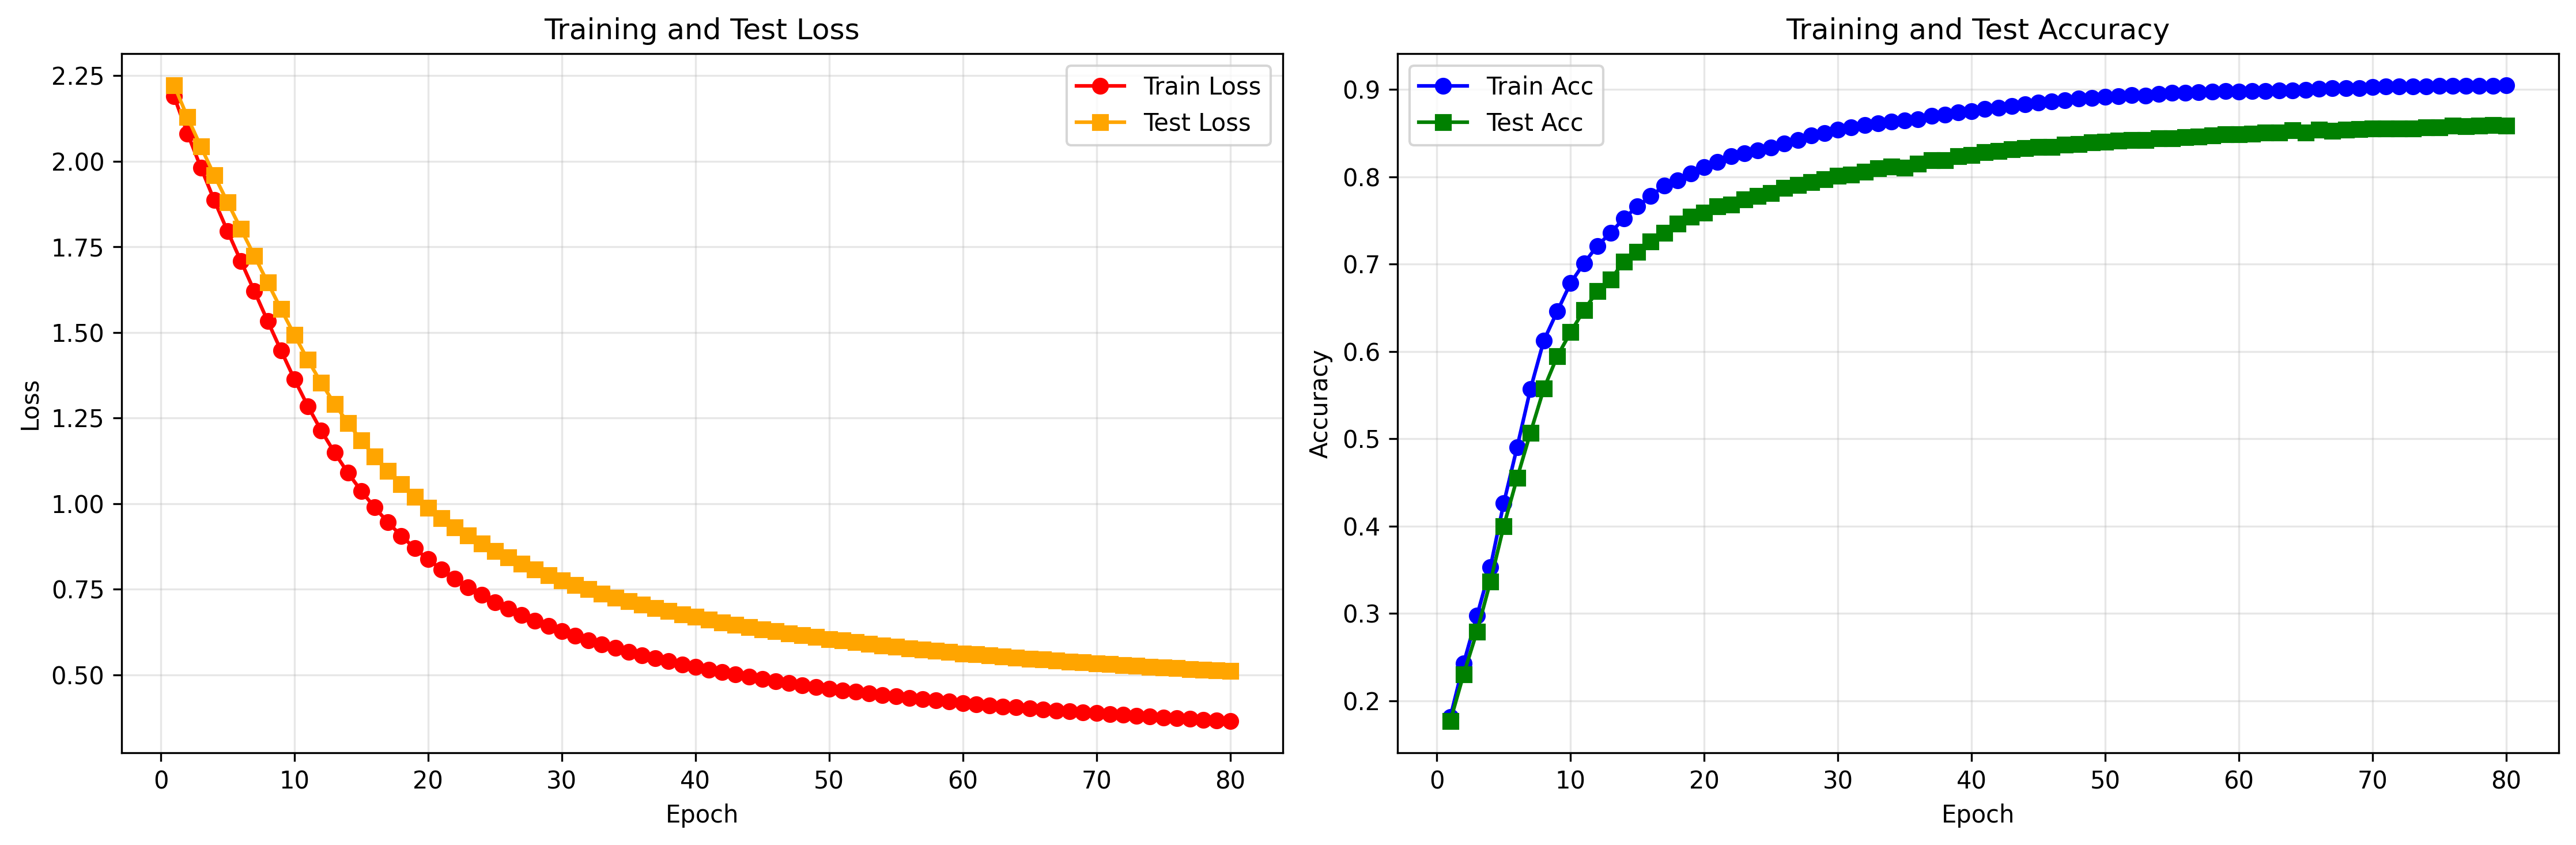
\includegraphics[width=0.8\textwidth]{../images/bpb.png}
    \caption{手写bp训练曲线}
    \label{fig:bp1}
\end{figure}
\begin{figure}[H]
    \centering
    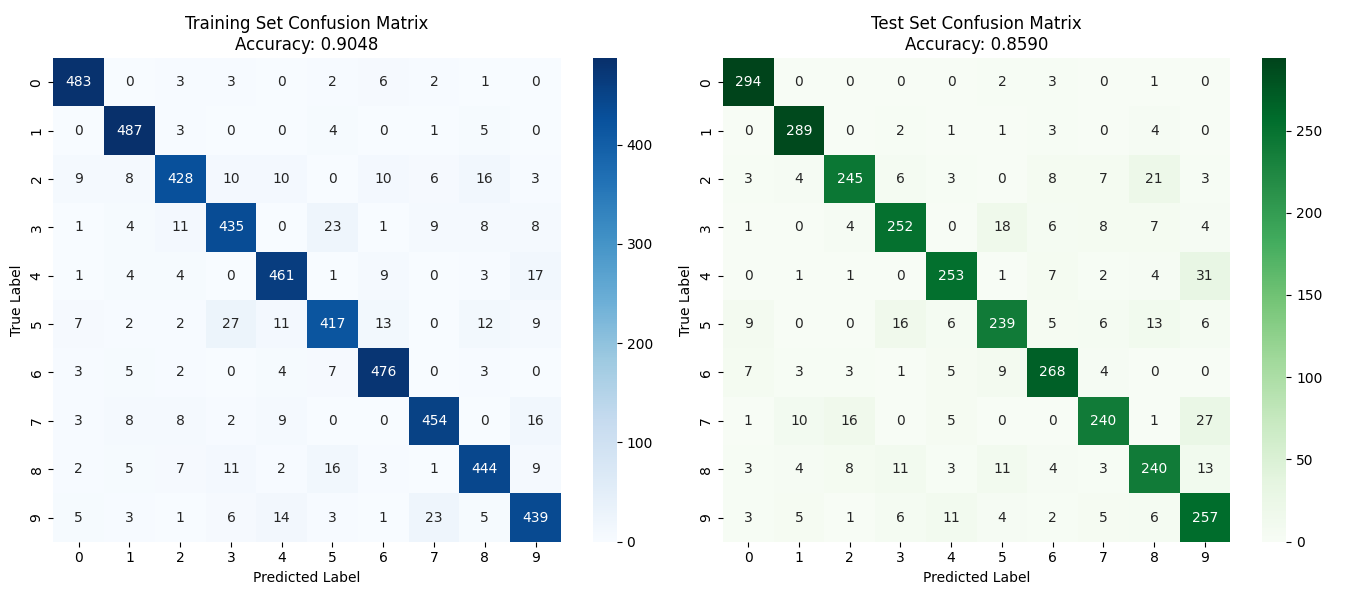
\includegraphics[width=0.8\textwidth]{../images/bpa.png}
    \caption{手写bp混淆矩阵}
    \label{fig:bp2}
\end{figure}
可以看到,多层感知机具有极强的拟合能力,仅仅一个隐藏层就能在该任务上达到不错的效果。
\subsection{实验二:隐层神经元的作用分析}
\subsubsection{实验设置}
本次实验旨在探索隐层神经元对模型的作用。实验依然采取了三层MLP模型,输入层、一个隐层和输出层。
我们设计了实验,逐渐增加隐藏层神经元个数,并在特定的轮次采用t-SNE方法对特征空间进行可视化,观察不同隐层神经元个数对特征聚类效果的影响。
为了实验方便与高效训练,我们使用了pytorch框架去实现后续的实验内容。实验的参数细节见表\ref{tab:training-config}。
\begin{table}[H]
\centering
\caption{MLP 模型训练参数配置}
\begin{tabular}{ll}
\toprule
\textbf{项目} & \textbf{配置} \\
\midrule
数据集        & MNIST 子集(每类训练样本 500,测试样本 300) \\
输入维度        & 784($28 \times 28$ 展平) \\
隐藏层维度范围  & $\{1, 2, 3, 4, 5, 6, 7, 8, 9, 10, 12, 14, 16, 32, 64, 128, 256\}$ \\
输出维度        & 10(数字类别) \\
激活函数        & ReLU \\
优化器          & Adam \\
学习率          & 0.001 \\
批大小          & 512 \\
训练轮数        & 共 80 轮 \\
损失函数        & CrossEntropyLoss(交叉熵) \\
记录 epoch 点   & \{0, 1, 3, 6, 10, 13, 20, 30, 60\}(包括初始状态) \\
特征可视化方法  & t-SNE(每 epoch 采样 500-800 条) \\
\bottomrule
\end{tabular}
\label{tab:training-config}
\end{table}

\subsubsection{结果分析}
\begin{figure}[H]
    \centering
    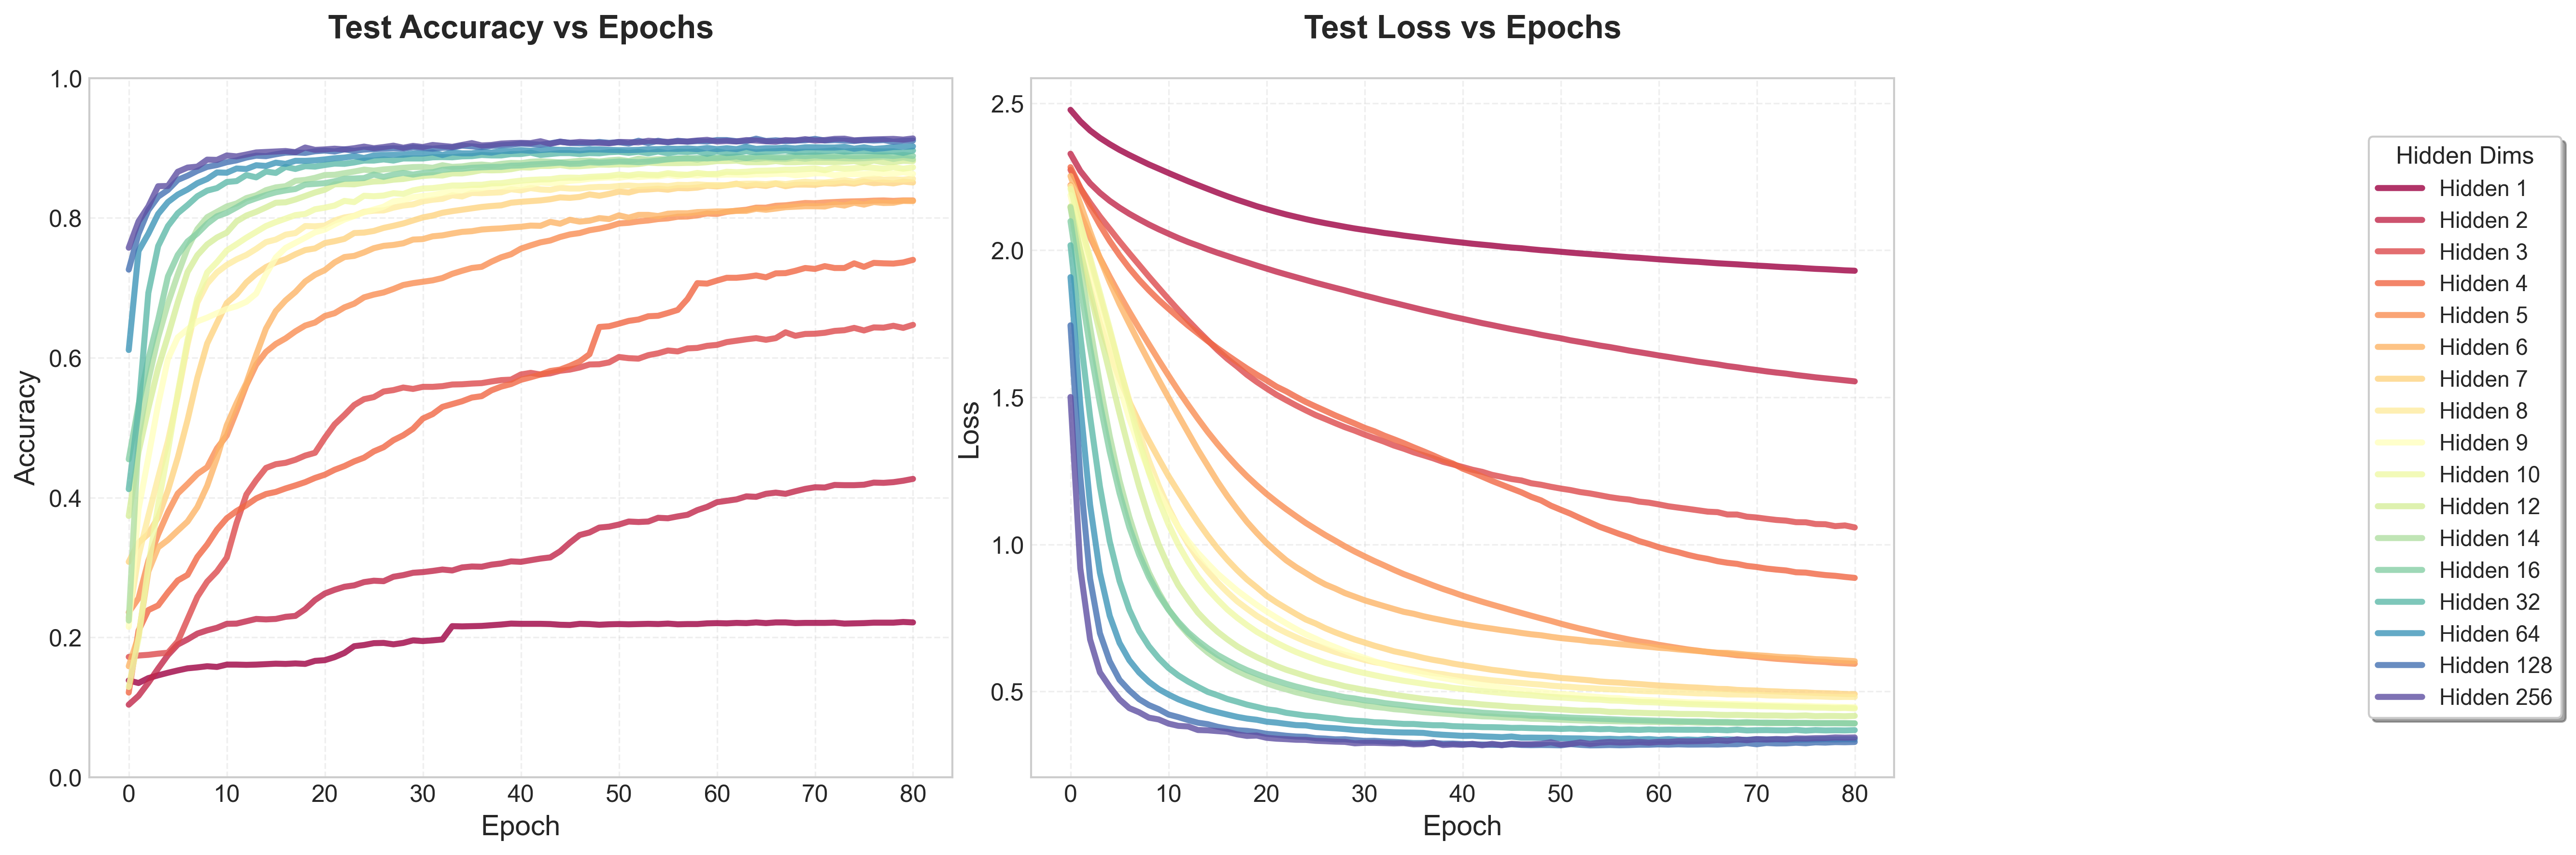
\includegraphics[width=0.8\textwidth]{../images/mlp_curves_Spectral.png}
    \caption{变更隐层神经元的acc与loss曲线}
    \label{fig:hidden}
\end{figure}
图\ref{fig:hidden}展示了不同隐层神经元个数下的训练准确率和损失曲线。我们可以观察到,当隐藏层神经元数量太少时,模型无法在给定的时间内得到较好的收敛结果。
由此,我们可以推断出,隐层神经元的数量对模型的拟合能力有着重要影响。随着隐层神经元数量的增加,模型的拟合能力也随之增强,但过多的神经元可能导致过拟合现象。

图\ref{fig:60}给出了epoch 60的时候,不同隐层神经元个数下模型特征空间的t-SNE可视化结果。可以看到,随着隐层神经元数量的增加,特征空间中的点簇聚类效果逐渐增强,表明模型对不同数字类别的区分能力在增强。
当隐层神经元数量较少的时候,模型无法在特征空间中写成较为分明的点簇,这反映了隐层神经元数目将直接影响模型的特征提取能力。
同时,特征空间的聚类效果也进一步揭示了神经网络学习能力的来源是训练特征提取器,实现在特征空间对数据的聚类效果。

图\ref{fig:8}展示了hidden layer神经元数目为8时,在不同轮次的t-SNE可视化结果。
我们可以观察到,最开始特征空间中点基本是散布的,几乎不存在明显的点簇。但是随着训练轮次的不断增加,我们逐渐观察到特征空间出现了明显的点簇聚类现象。
这再次印证了神经网络的训练过程与特征空间点簇聚类效果的密切关系。
\begin{figure}[h]
    \centering
    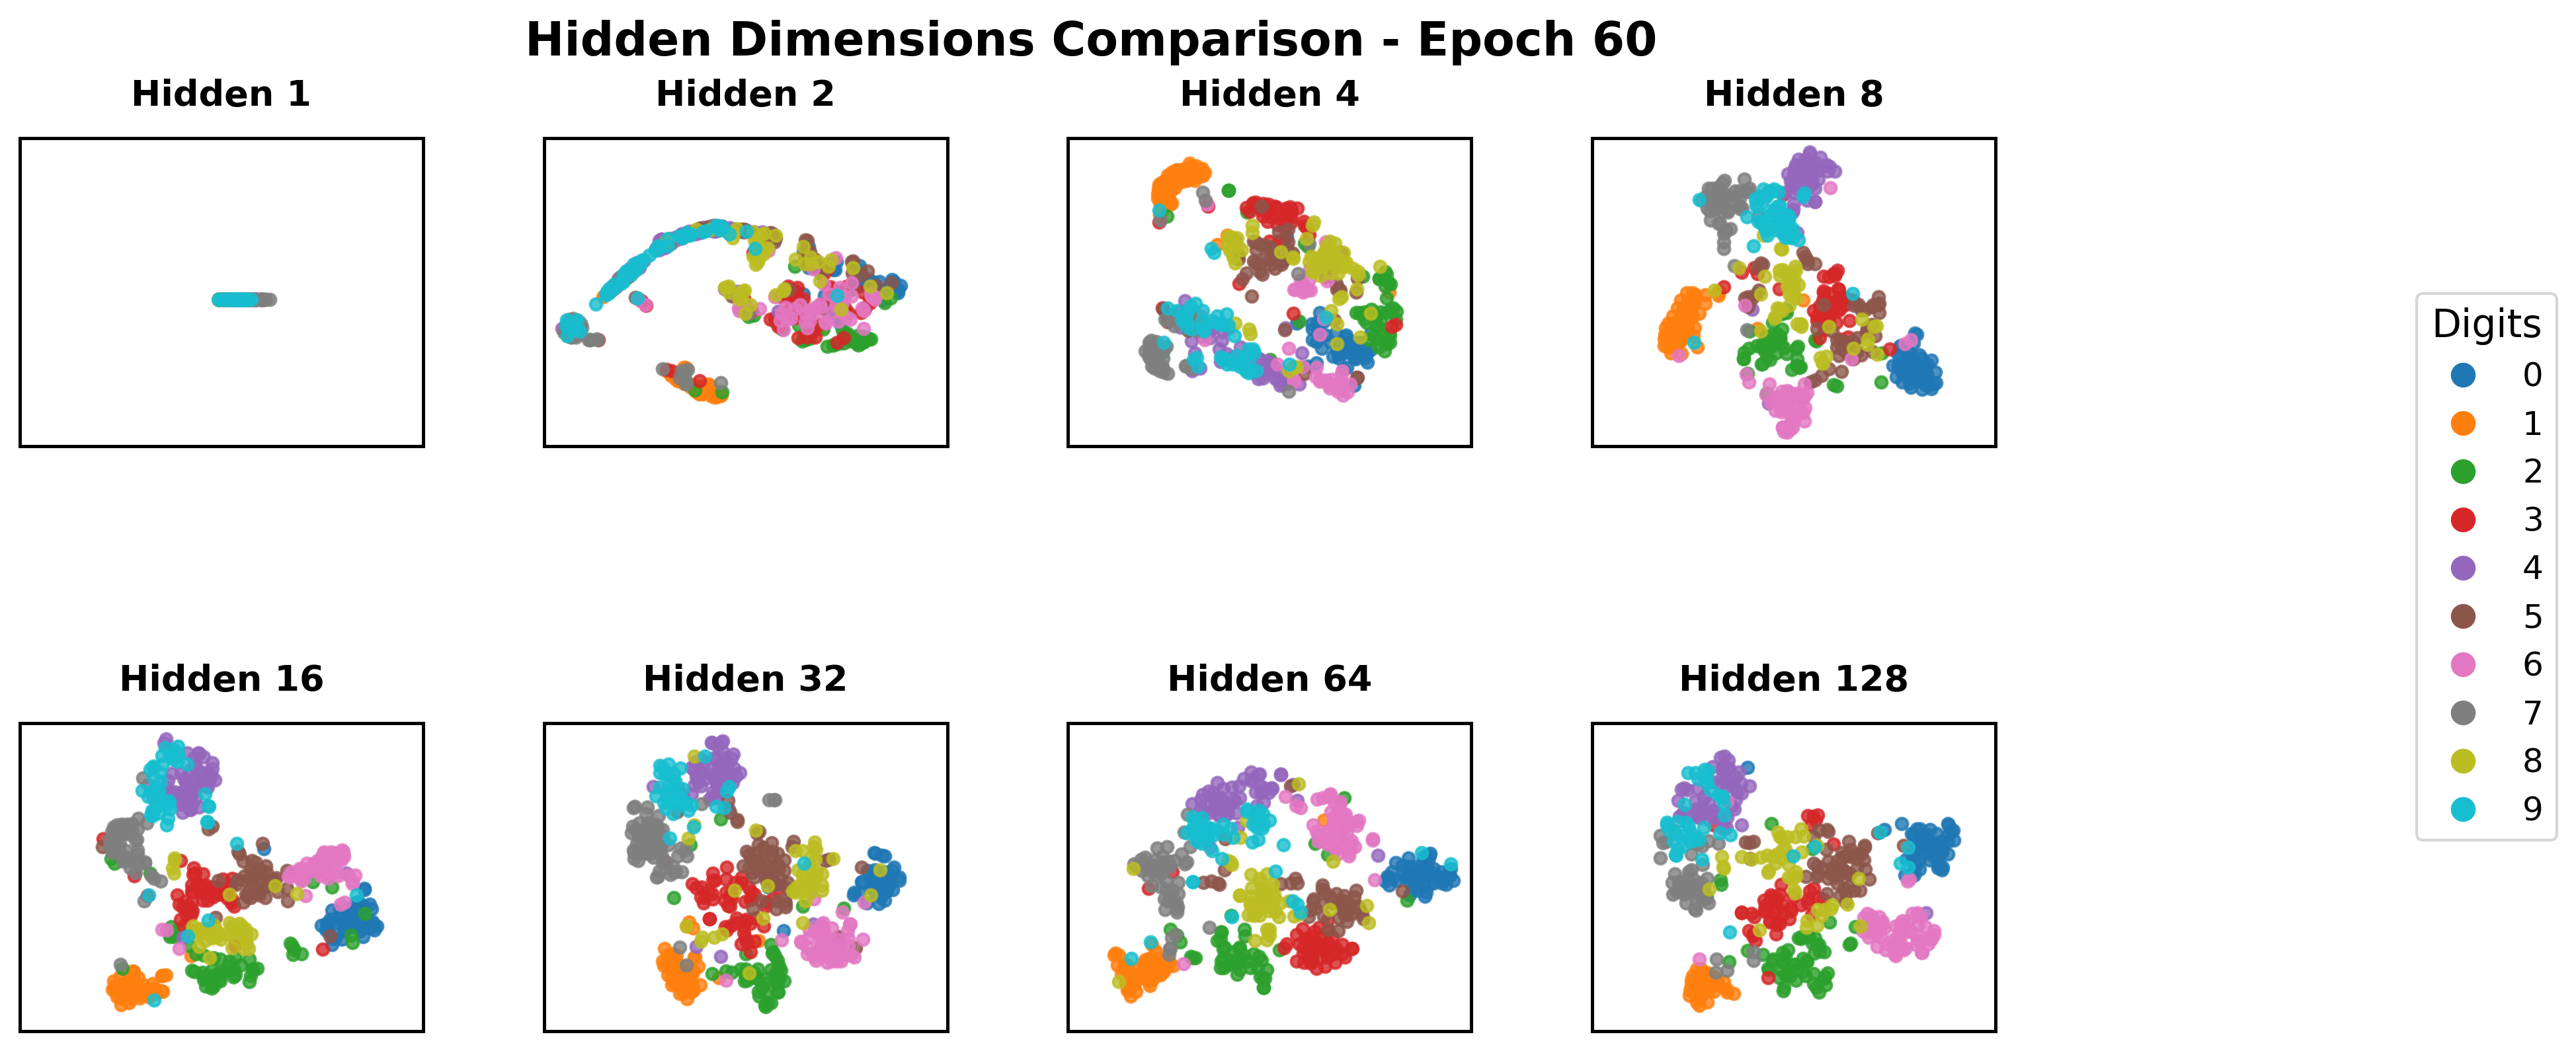
\includegraphics[width=0.8\textwidth]{../images/pa/tsne_comparison_epoch_60.png}
    \caption{同轮次,不同模型的t-SNE可视化结果}
    \label{fig:60}
\end{figure}

\begin{figure}[h]
    \centering
    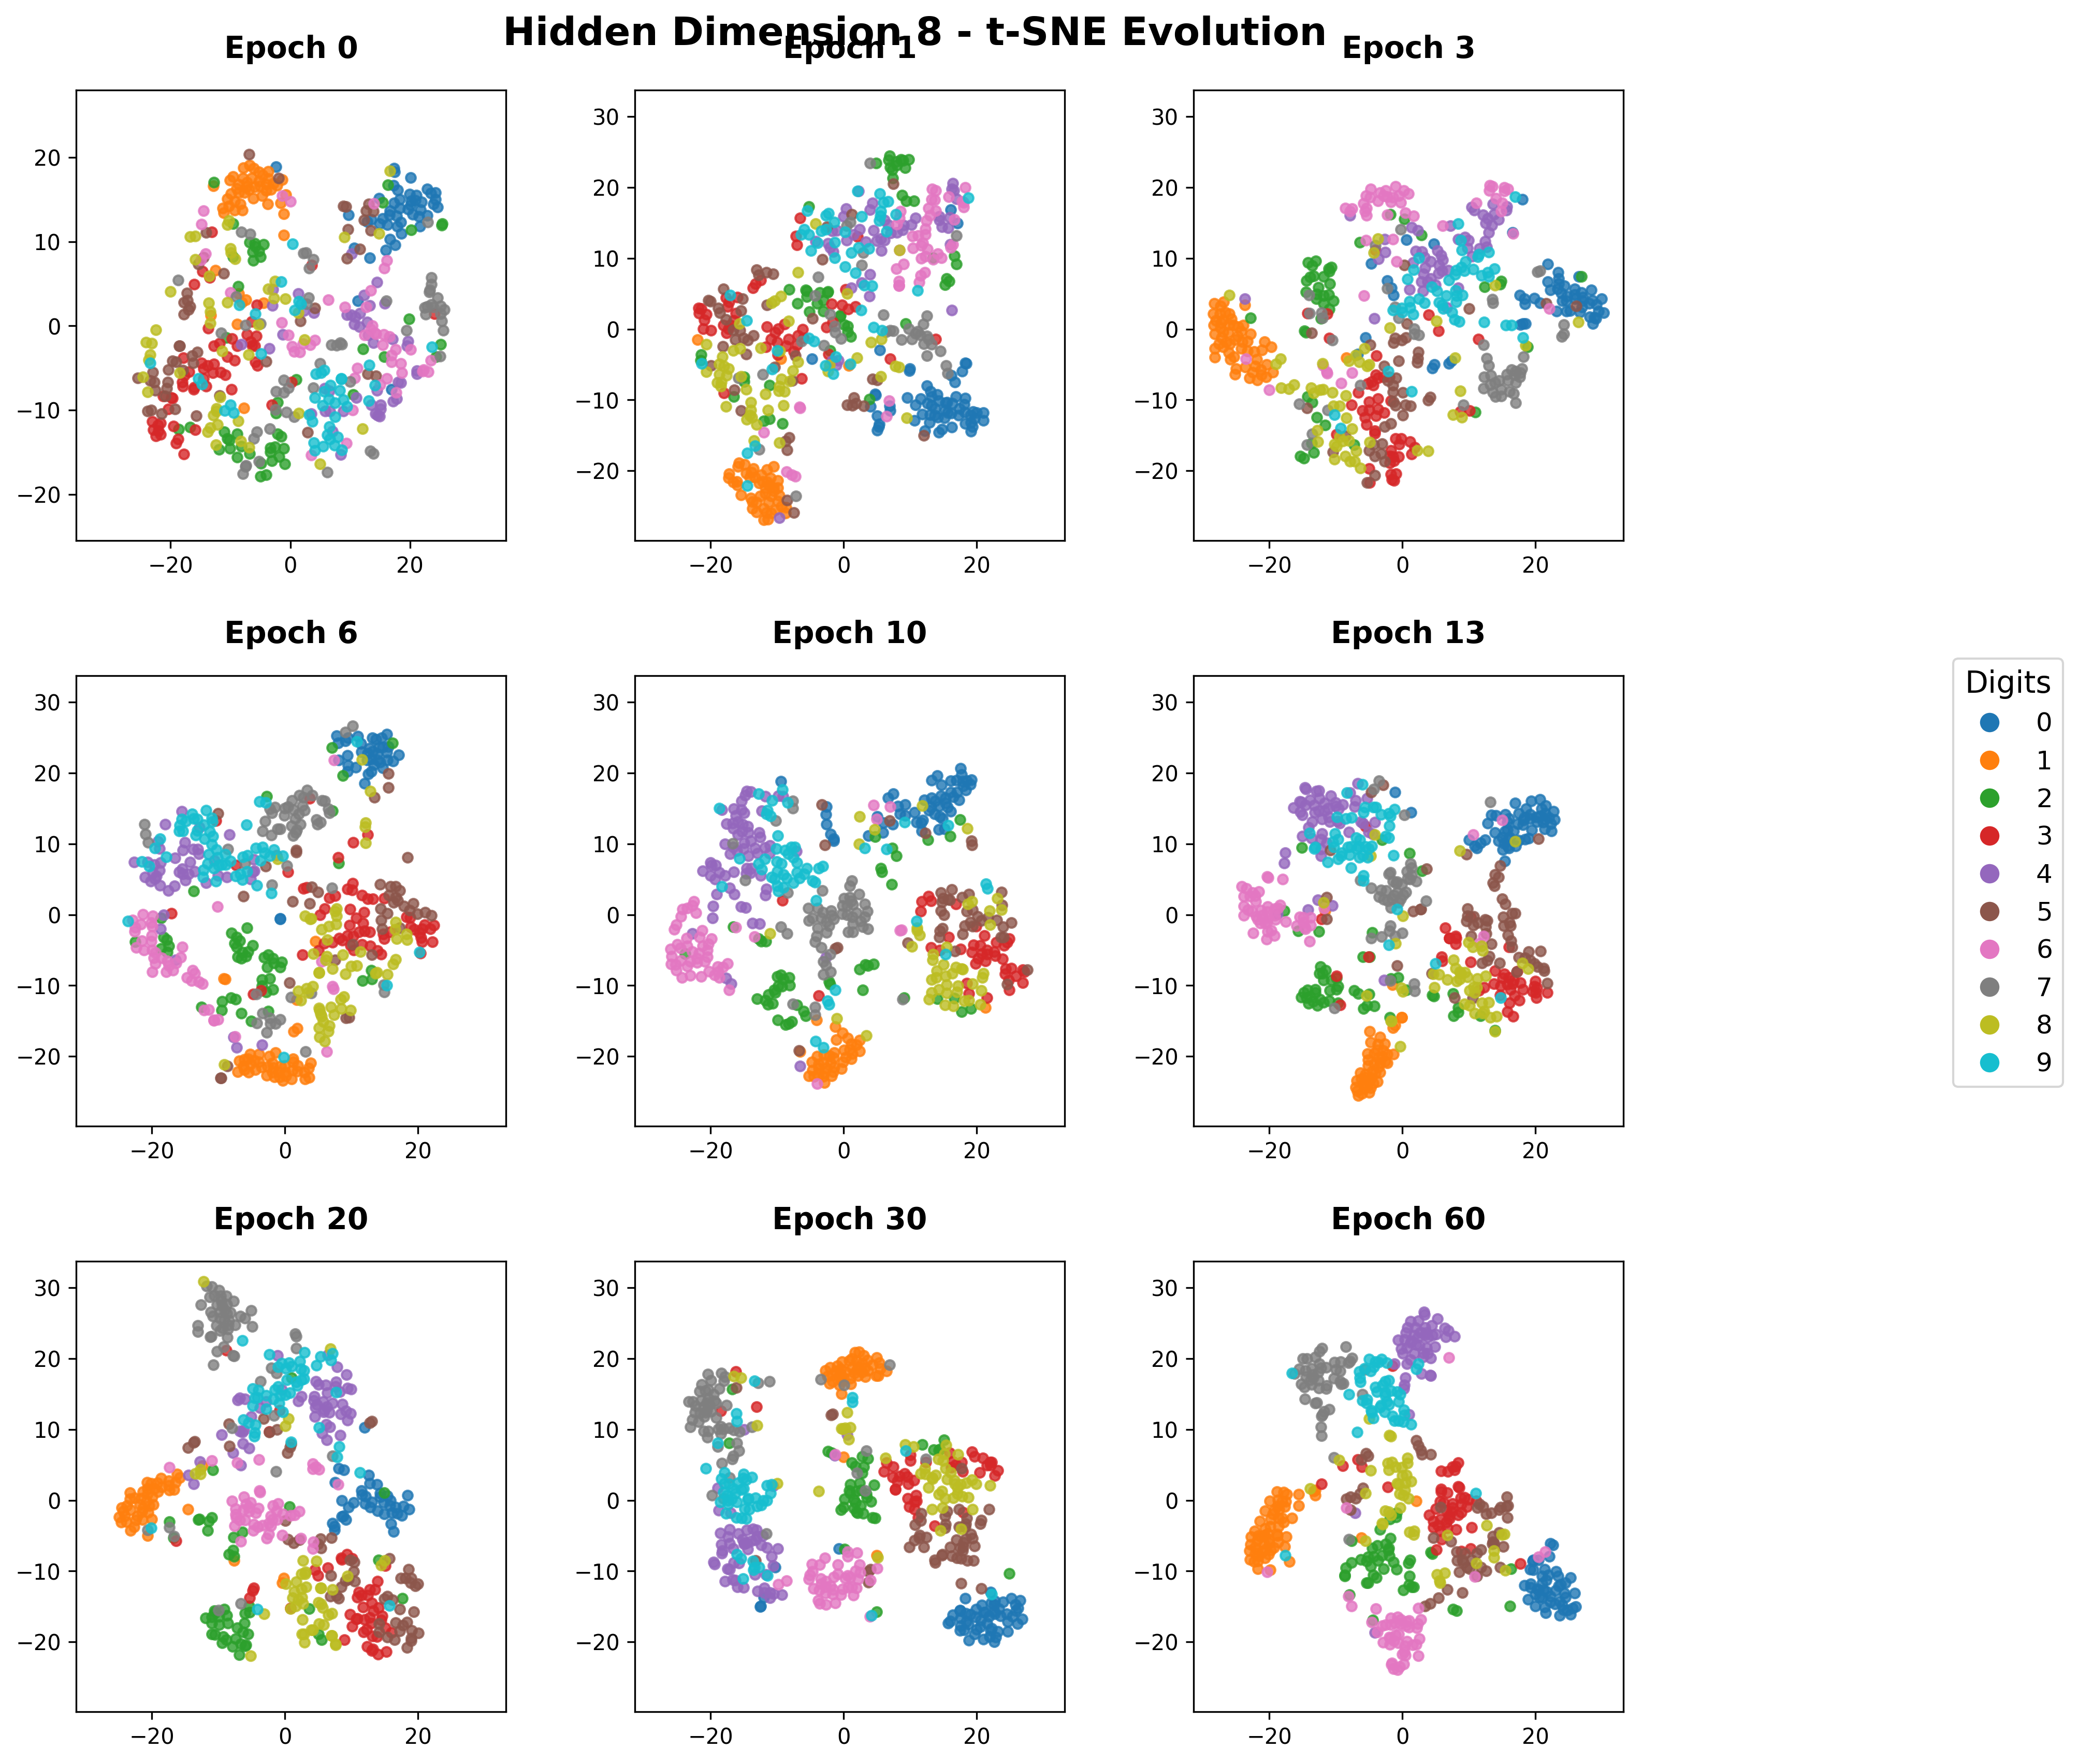
\includegraphics[width=0.8\textwidth]{../images/pa/tsne_evolution_hidden_8.png}
    \caption{同模型,不同轮次的t-SNE可视化结果}
    \label{fig:8}
\end{figure}
我们完成了实验设计中的所有实验,更多的实验结果见附录\ref{sec:hidden}。

\subsection{实验三:特征提取器与分类器的解耦分析}
\subsubsection{分析思路}
参照图\ref{fig:mlpstructure}中神经网络的结构,神经网络可以被分割为两部分,第一部分是前半段,负责数据特征的提取,把数据从高维空间映射到相对较低维度的特征空间;第二部分实现从特征空间到标签空间的映射,完成分类任务。
我们大胆而又不失理智地认为,神经网络的前后两部分承担了完全不同的功能。即前半部分负责特征提取,后半部分负责学习从特征到分类的映射。
为了表达方便,我们后面都将前半部分称为特征提取器(Feature Extractor),后半部分称为分类器(Classifier)。

我们进而又有新的想法,随机初始化的分类器权重,实质上已经显示定义了一个从特征空间到标签空间的映射关系。
我们有理由相信,对于这组随机初始化的分类器权重参数,当我们把目光投到广阔的高维特征空间中时,我们总能找到一个又一个的区域成为数据理想的特征投射范围。
由此,我们大胆地认为,当隐层神经元数目够多的时候,分类器没有训练的必要,我们只需要让特征提取器去适应分类器权重所定义的“合理特征投射域”即可。
\subsubsection{实验设置}
总体上我们的实验参数设计与表\ref{tab:training-config}一致。

但是在实验部署上,我们只对$\{1,8,16,32,64,128,256\}$这七组隐层神经元数目进行了实验。
实验内容有三个部分:正常训练,冻结特征提取器权重,冻结分类器权重。
我们绘制acc与loss曲线,观察冻结特征提取器与冻结分类器对模型训练的影响。
以期验证我们的猜想。

\subsubsection{实验结果分析}
本实验结果过长,见附录\ref{sec:feature_extractor_classifier}。
我们发现,在隐层神经元为1的时候,冻结分类器甚至能带来更好的效果,这是十分令人震惊的,我们目前没有找到好的解释。
分析后续的图,我们发现,冻结分类器的loss曲线总是在正常训练上方,但是有意思的一点是,随着隐层神经元个数增多,两条loss的距离是越来越近的(橙色与蓝色),这也证实了我们的大胆猜想,
即当隐层神经元数目足够多的时候,我们完全可以依靠强大的特征表示能力,让特征空间对齐分类器随机初始化的权重。
同时,冻结特征提取器权重的loss总是显著高于冻结分类器的loss和正常训练的loss,这也再次印证了特征提取器的作用是不可或缺的。

\section{卷积神经网络}

\subsection{模型架构与实验设置}

本实验中采用一个简单的卷积神经网络(SimpleCNN)对 MNIST 手写数字图像进行分类。模型结构如下表所示:

\begin{table}[H]
  \centering
  \caption{CNN 模型结构设计}
  \begin{tabular}{lccc}
    \toprule
    层名称 & 操作类型 & 输出尺寸 & 参数说明 \\\midrule
    输入     & -               & $1 \times 28 \times 28$ & 灰度图像输入 \\\midrule
    Conv1    & 卷积层         & $8 \times 28 \times 28$ & 卷积核 $5\times5$, padding=2 \\
    ReLU1    & 激活函数       & $8 \times 28 \times 28$ & ReLU 激活 \\
    Pool1    & 最大池化层     & $8 \times 14 \times 14$ & 池化核 $2\times2$, stride=2 \\\midrule
    Conv2    & 卷积层         & $16 \times 14 \times 14$ & 卷积核 $5\times5$, padding=2 \\
    ReLU2    & 激活函数       & $16 \times 14 \times 14$ & ReLU 激活 \\
    Pool2    & 最大池化层     & $16 \times 7 \times 7$ & 池化核 $2\times2$, stride=2 \\\midrule
    Flatten  & 展平操作       & $784$ & $16 \times 7 \times 7$ 展平为一维向量 \\
    FC       & 全连接层       & $10$ & 输出10类得分,对应0-9数字 \\
    \bottomrule
  \end{tabular}
  \label{tab:cnn-structure}
\end{table}

整个网络具有两层卷积模块,均包含卷积、ReLU 激活和最大池化操作,最后通过全连接层输出10个类别的预测结果。该结构在保持计算效率的同时,具有良好的特征提取能力,适用于对 MNIST 这类简单图像数据集的分类任务。

\subsection{实验结果}

为了理解卷积神经网络在图像识别任务中的特征提取机制,我们对模型中两个卷积层的中间输出进行了特征图(feature maps)可视化,如图 \ref{fig:conv1_feat} 和图 \ref{fig:conv2_feat} 所示。

\begin{figure}[H]
  \centering
  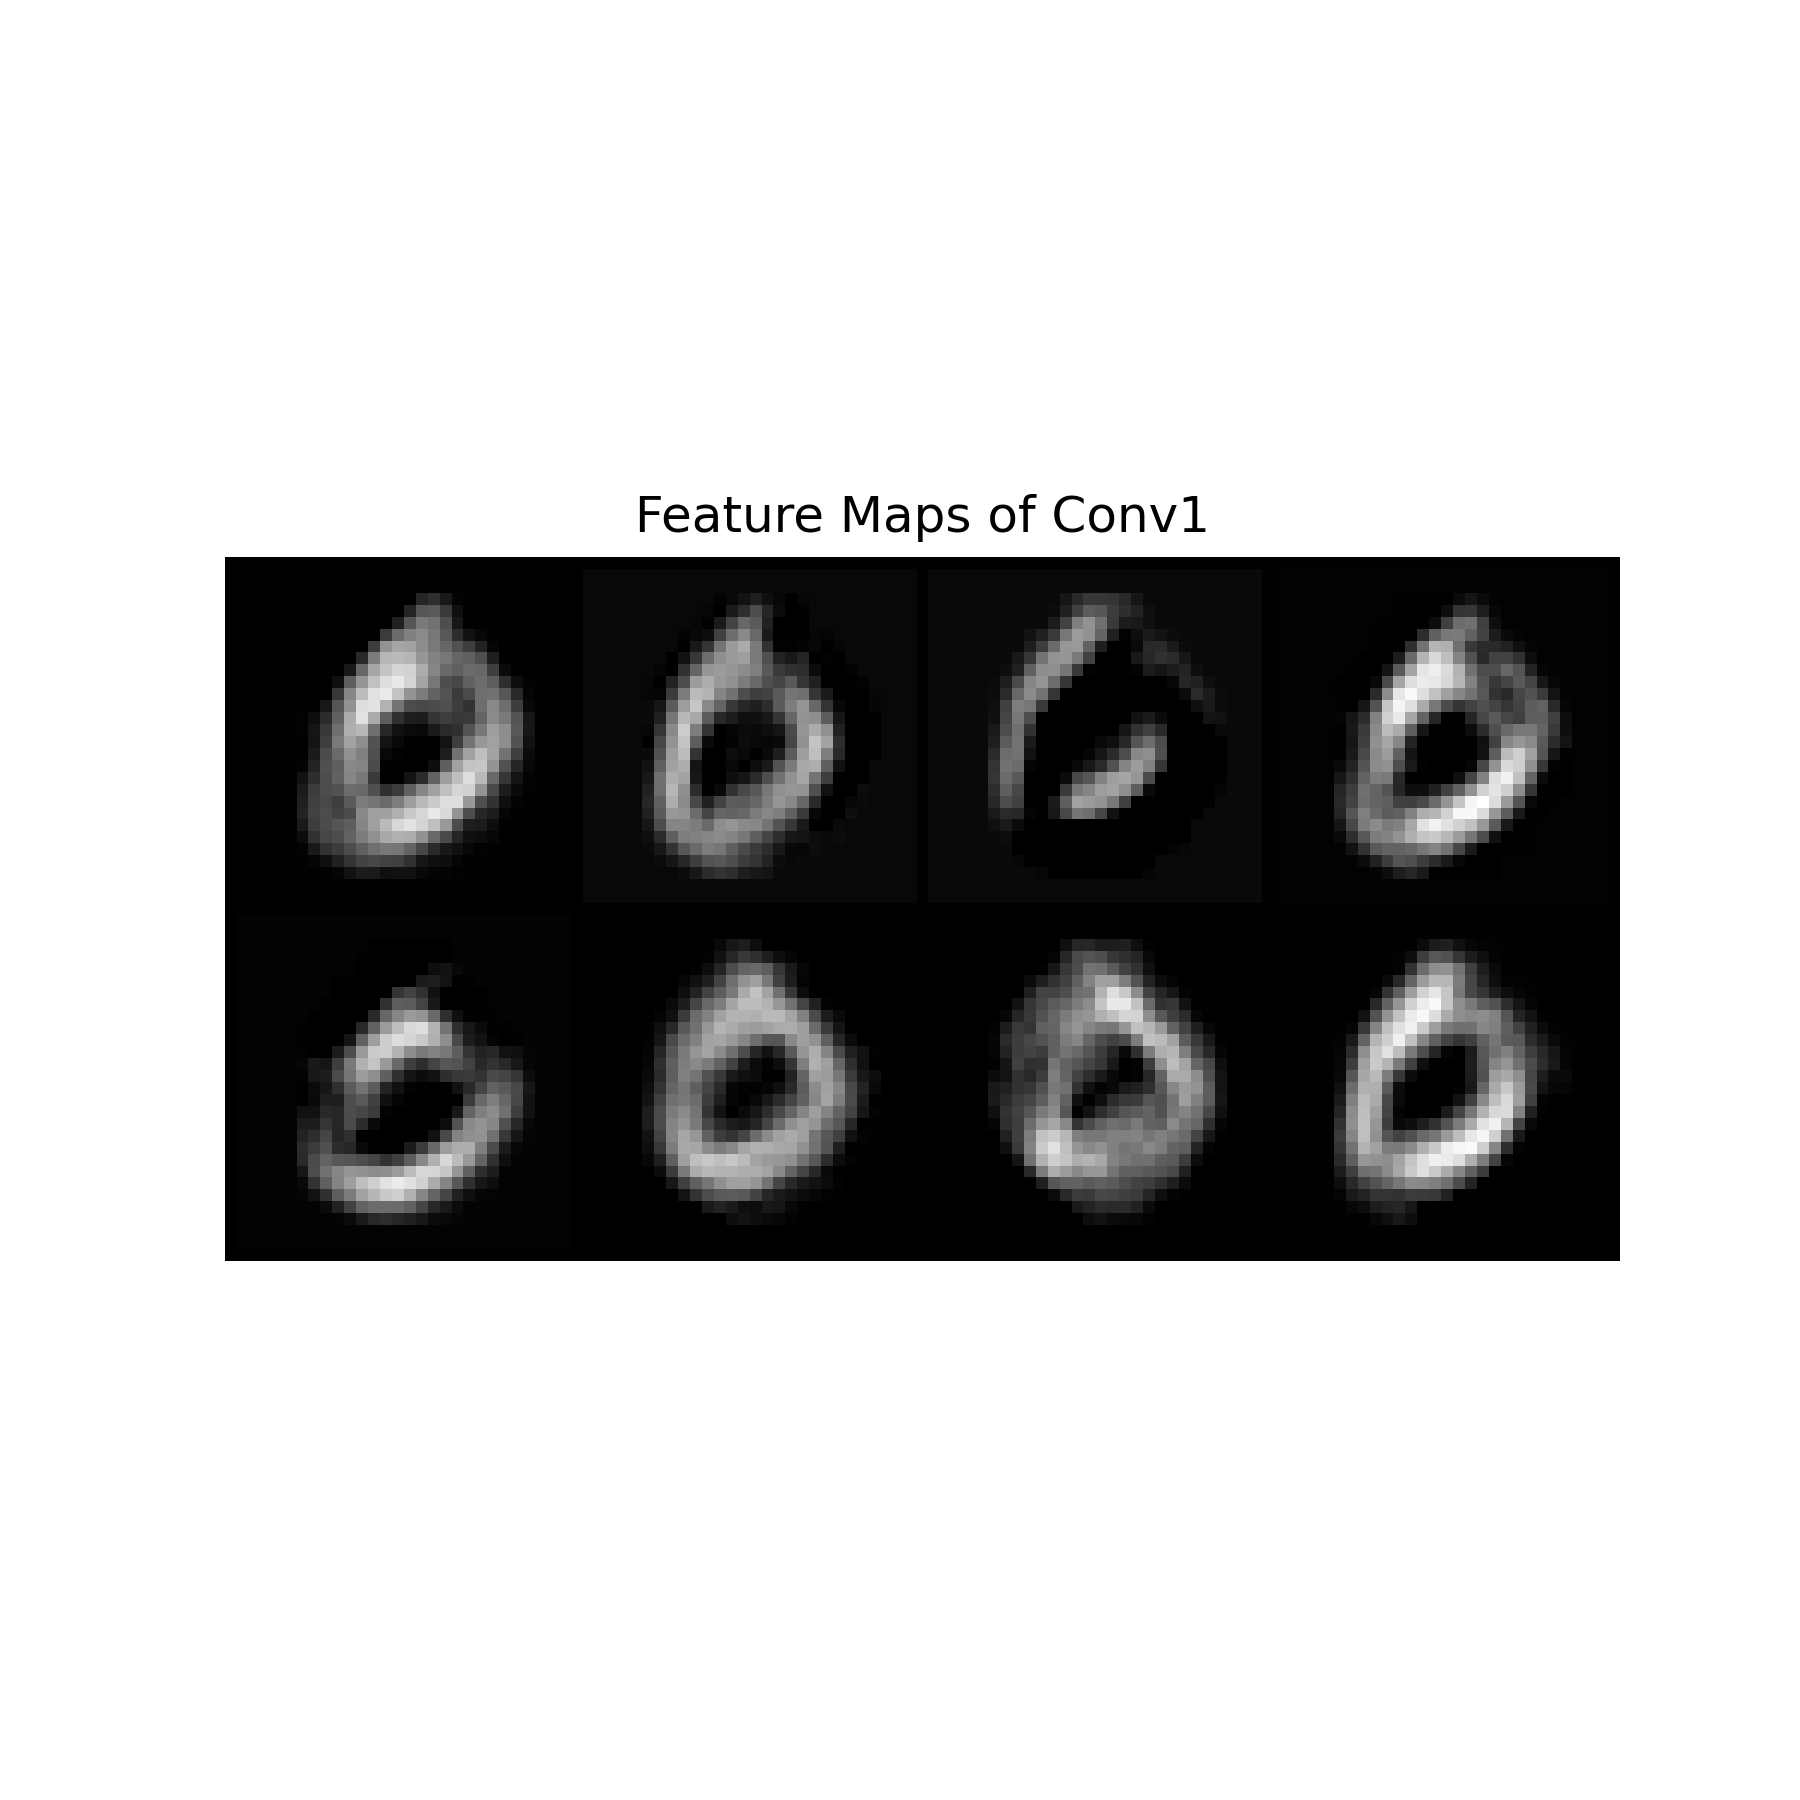
\includegraphics[width=0.4\textwidth]{../images/cnn/Conv1_feature_maps.png}
  \caption{第一层卷积层(Conv1)输出的特征图}
  \label{fig:conv1_feat}
\end{figure}

\begin{figure}[H]
  \centering
  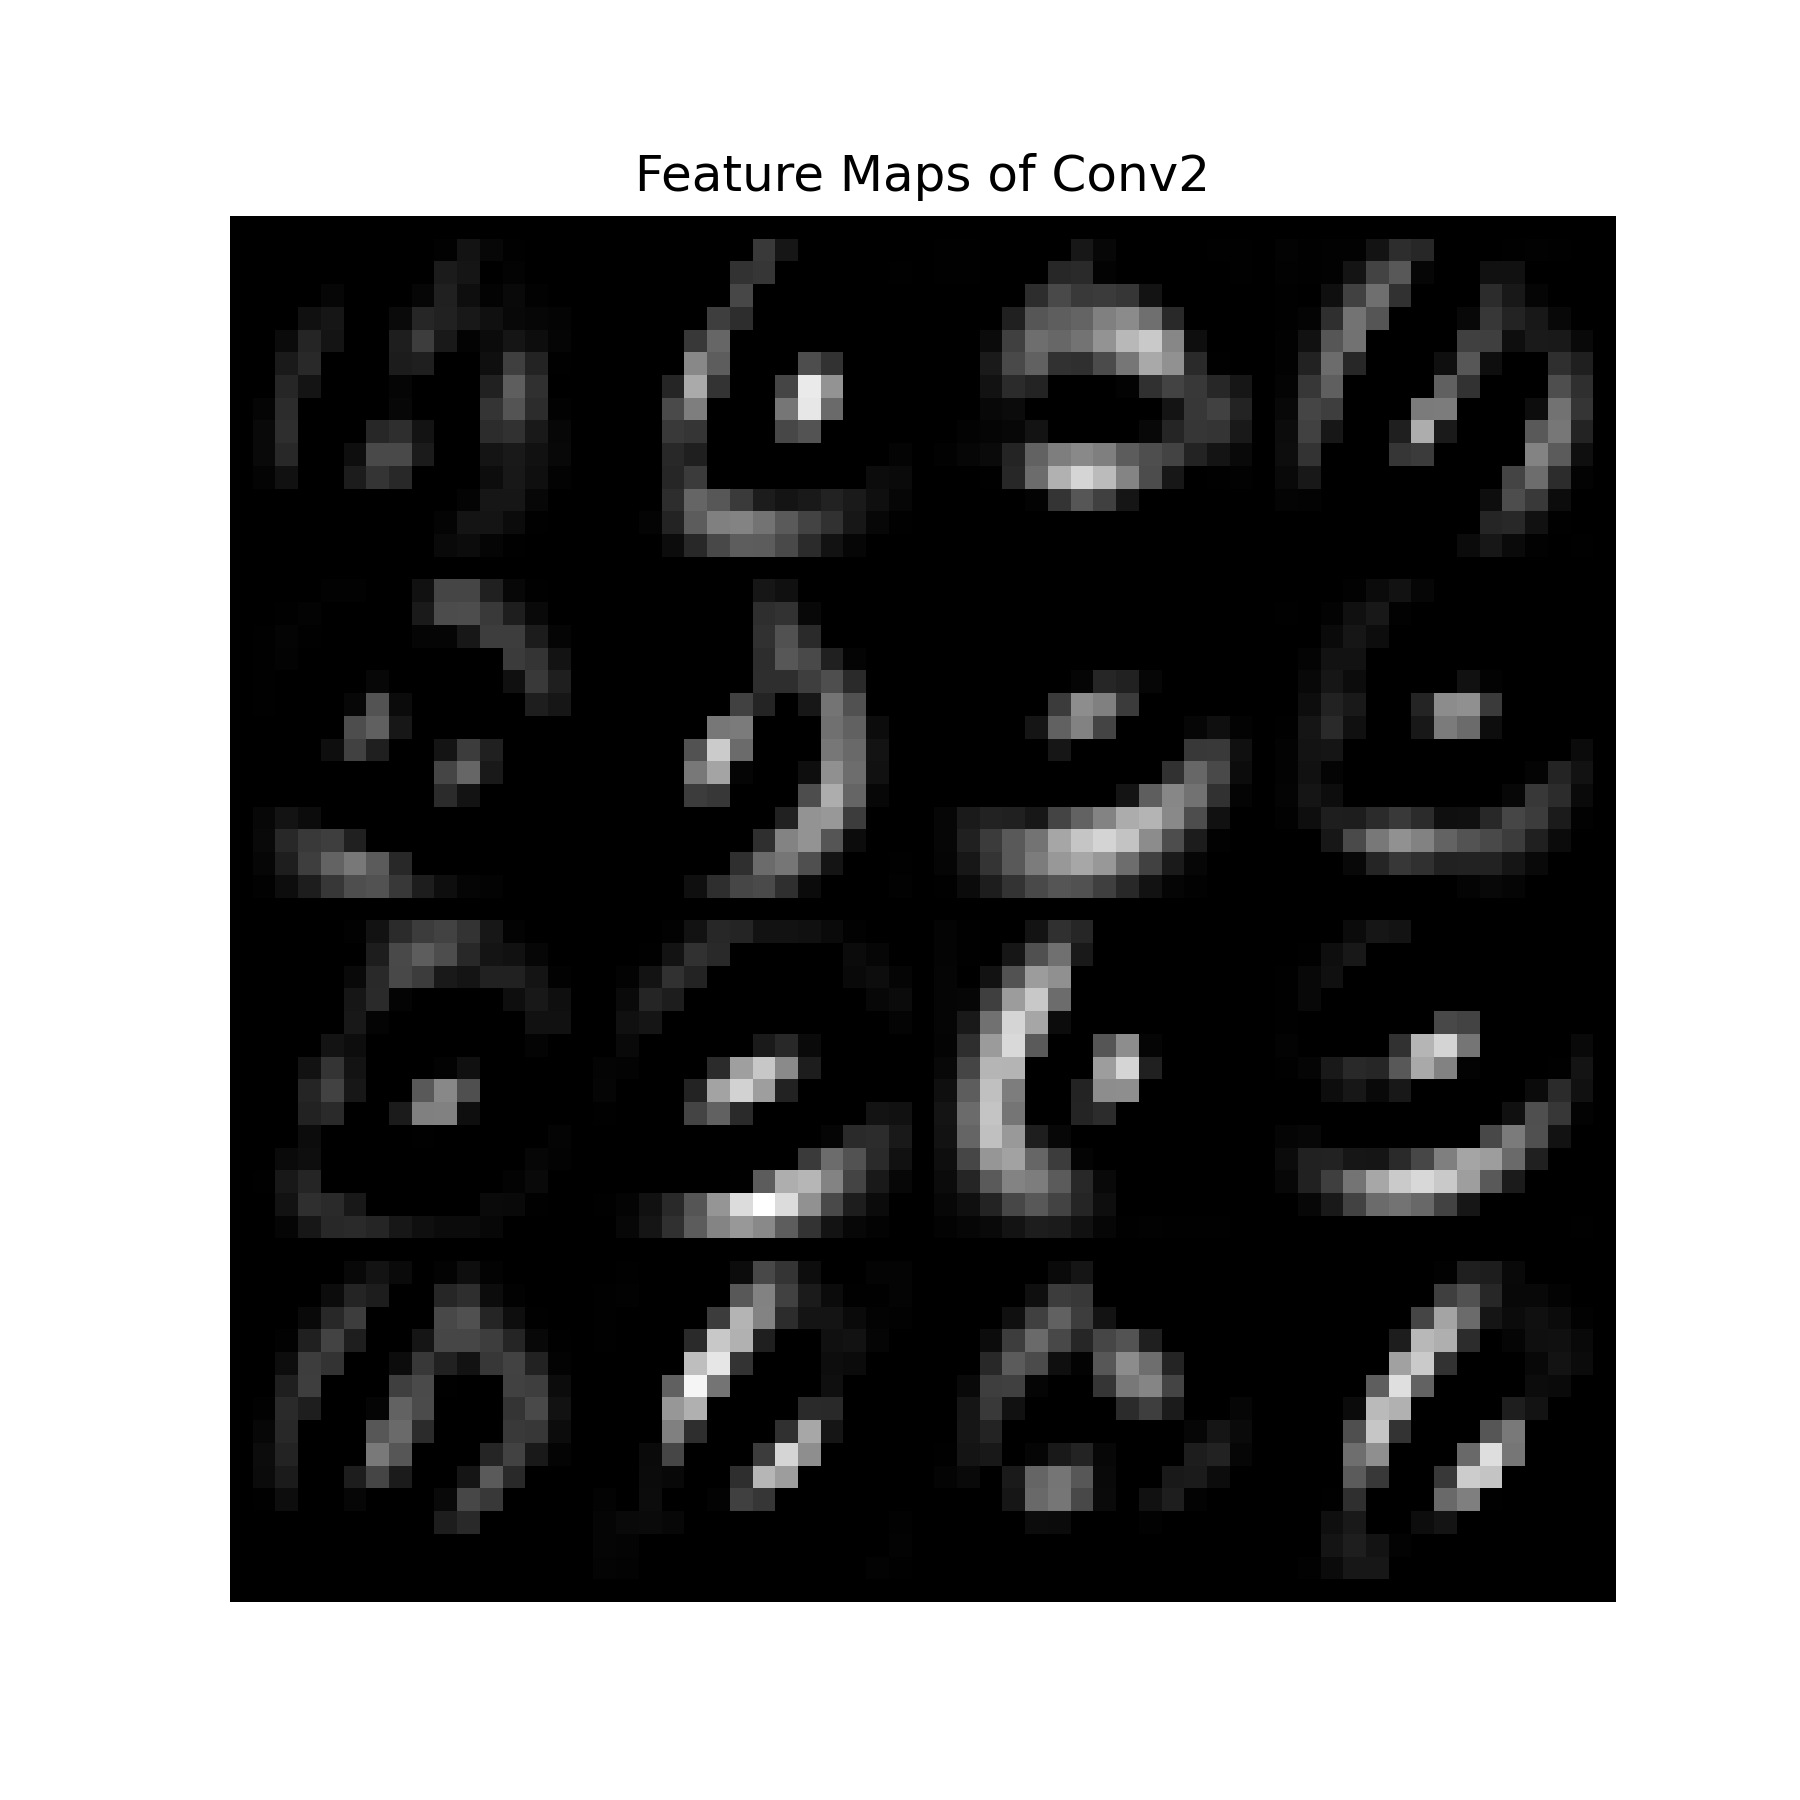
\includegraphics[width=0.4\textwidth]{../images/cnn/Conv2_feature_maps.png}
  \caption{第二层卷积层(Conv2)输出的特征图}
  \label{fig:conv2_feat}
\end{figure}

上述特征图是模型在处理一张测试图像(MNIST 数据集中某个数字)时,各卷积核输出的中间结果。
从图中可以观察到:
\begin{itemize}
  \item 第一层卷积(图 \ref{fig:conv1_feat})提取的是较为底层的边缘、线条等基础纹理特征,图像结构清晰,部分通道高亮了边缘或笔画起笔处;
  \item 第二层卷积(图 \ref{fig:conv2_feat})抽取的是更高阶的组合特征,包含了曲线、封闭环状区域或笔画连接区域,特征图相比更抽象且稀疏;
\end{itemize}

\textbf{特征图可视化的意义在于}:帮助我们理解模型在中间层是如何逐步从像素信息中构建“语义特征”的,从而增强了模型可解释性。这对于模型调试、结构设计、以及对错误样本的分析具有重要参考价值。


\section{探索:神经网络是记忆还是学习?}
视觉是生物智能的一个基本体现,然而机械结构的神经网络在手写数字识别上已经展现出了与人类不相上下的能力,我们不禁要发出疑问,神经网络到底是真的“学习”到了如何识别一个数字,还是仅仅是因为记住了大量样例而表现出了伪智能性质呢?

回顾对数据集像素统计特征的分析\ref{fig:xd},数据集几乎不存在偏离图像中心的样本。
我们设计了一个交互式平台进行实验,测试模型对偏离中心样本以及对不同笔画粗细样本的识别能力。
\begin{figure}[H]
    \centering
    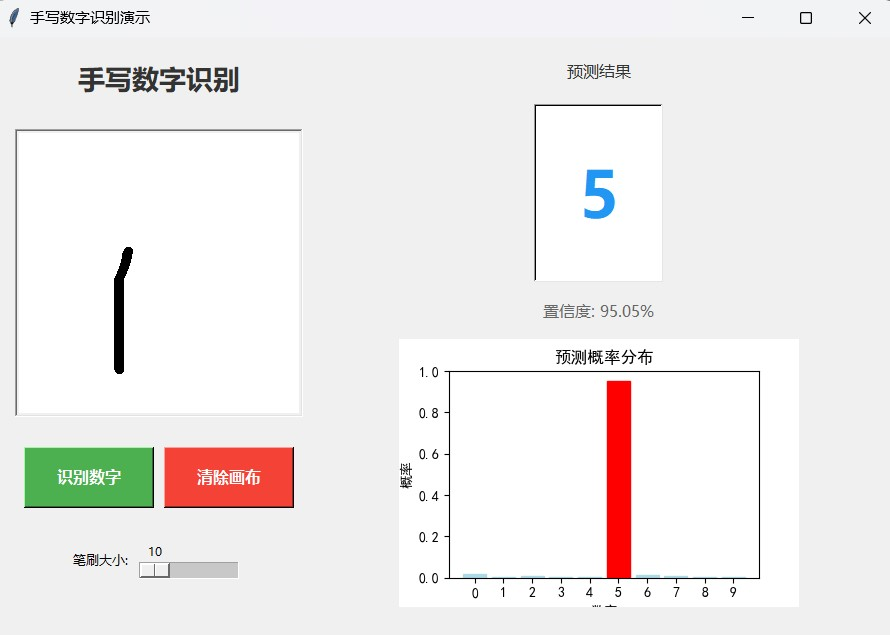
\includegraphics[width=0.8\textwidth]{../images/mlp/2025-06-21 063508.jpg}
    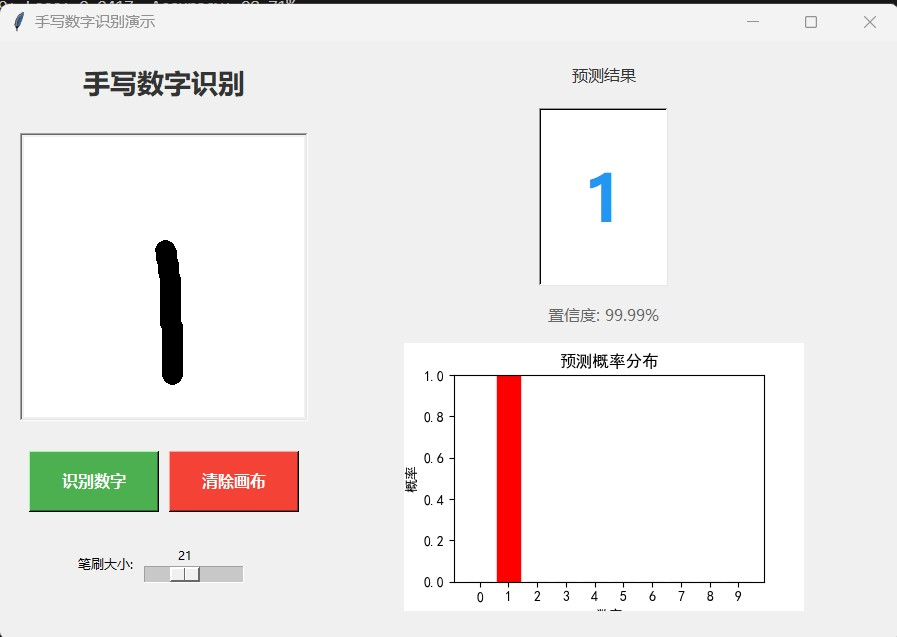
\includegraphics[width=0.8\textwidth]{../images/mlp/2025-06-21 063540.jpg}
    \caption{mlp交互式测试平台}
    \label{fig:interactive}
\end{figure}
\begin{figure}[H]
    \centering
    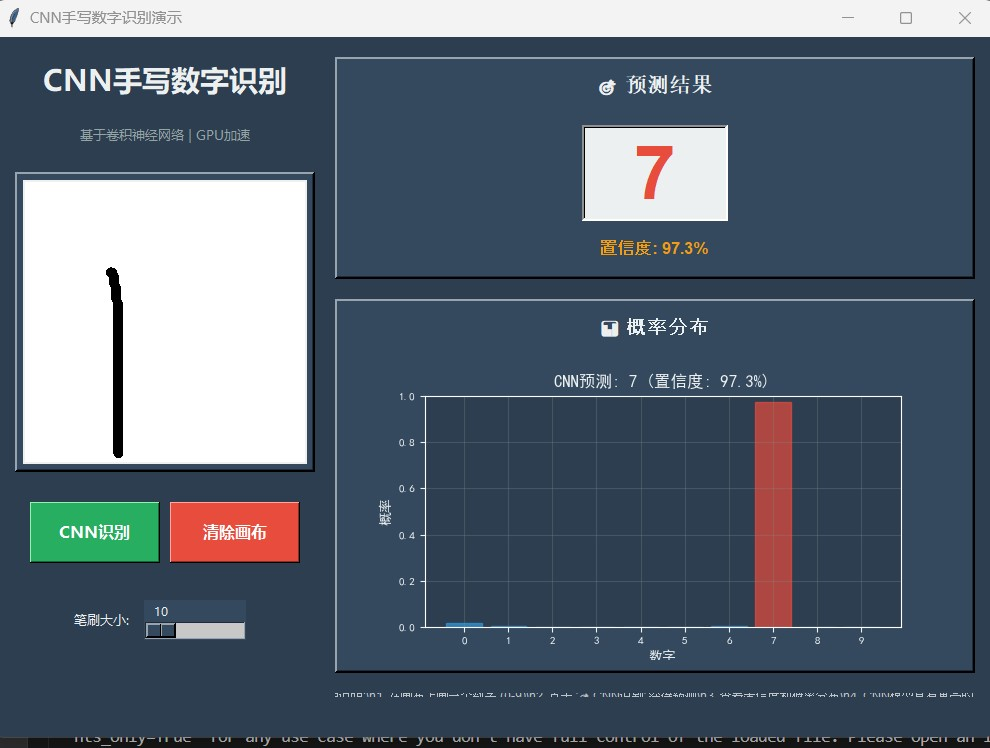
\includegraphics[width=0.8\textwidth]{../images/cnn/2025-06-21 063623.jpg}
    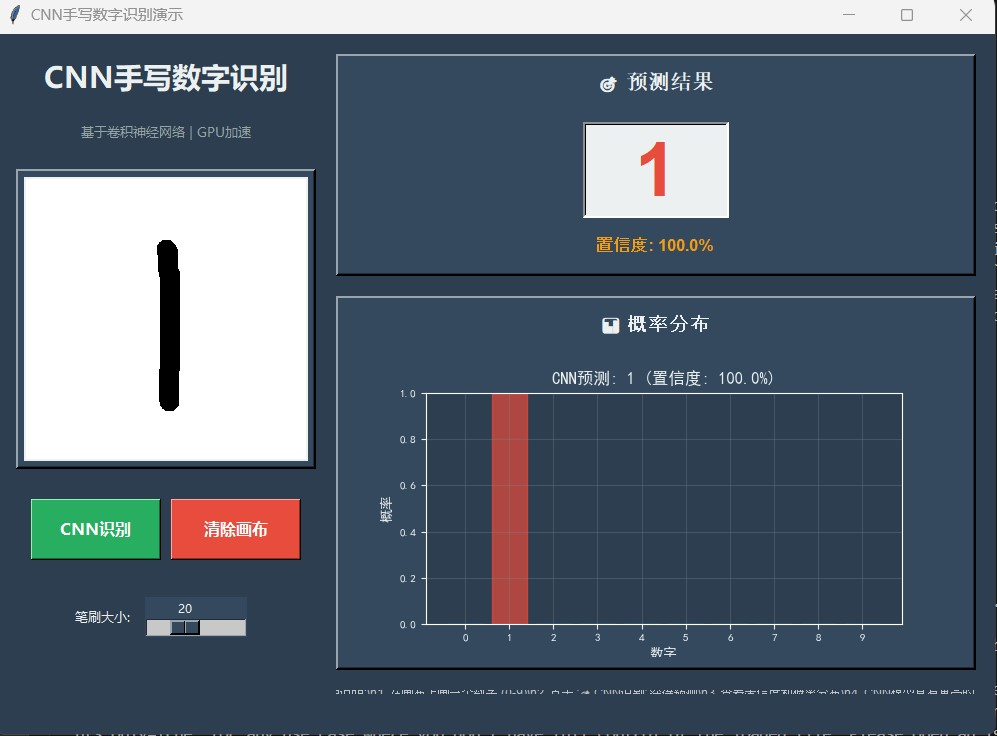
\includegraphics[width=0.8\textwidth]{../images/cnn/2025-06-21 063651.jpg}
    \caption{cnn交互式测试平台}
    \label{fig:interactive1}
\end{figure}
如上所示,无论是mlp还是cnn,模型都只是学会了针对数据集的识别模式,而并没有真正学会如何识别一个数字。
综上,我们认为模型的识别能力并非真正的“学习”,而是对数据集模式的记忆。

\section{结语}
本文围绕手写数字识别这一经典任务,系统性地分析了神经网络在该任务中的建模能力与行为机制。我们并没有痴迷于套壳更大更强的模型,这在手写数字这一任务上是无意义的,相反,我们深入挖掘了神经网络的特征提取与分类能力,尝试揭示其“学习”本质。

我们从最基础的多层感知机(MLP)出发,首先实现了一个手动反向传播模型,深入理解了网络训练过程中的参数更新机制;随后,我们探索了隐层神经元数量对模型性能与特征空间聚类效果的影响,并通过 t-SNE 降维可视化加深了理解。

进一步地,我们将神经网络视作特征提取器与分类器的组合结构,设计了参数冻结实验,验证了“特征空间对齐分类器”的假设。最后,我们训练了简单的卷积神经网络,并可视化其中间特征图,直观展示了卷积操作在多层网络中的语义抽象过程。

我们发现,神经网络的强大能力并非仅来源于其“深”或“宽”,而是来自其能在训练数据上自发构造出有判别性的特征空间——这是其“学习能力”的真正体现。然而,我们也注意到:在数据分布非常集中、样本缺乏变化性时,模型往往只是“记住”了数据结构,而非真正学会了数字本质。

这引发了我们一个问题:当我们说“神经网络学会了识别数字”,我们是否真的知道,它是如何知道“这就是数字 3”?或者说,是否只是知道“这类结构常出现在 3 所在的训练数据中”?这也许正是下一阶段我们所要深入探究的问题。

通过这次实验,我们的组员在不断地交流与实践中深化了对神经网络的理解,以手写数字识别这一基础任务为切入点,探索了神经网络的特征提取与分类能力。未来,我们希望能在更复杂的任务上,继续验证这些理论,并进一步揭示神经网络的内在机制。

\newpage

% 参考文献
\bibliographystyle{plainnat}
\bibliography{ref}



\newpage
\appendix

\section{反向传播算法}

\subsection{多层感知机反向传播}\label{sec:mlpbp}

在多层感知机(MLP)中,我们令网络共有 $L$ 层,第 $l$ 层的参数为权重矩阵 $W^{(l)}$ 和偏置向量 $b^{(l)}$。对于输入样本 $(x,y)$,定义:
\[
\begin{aligned}
&z^{(l)} = W^{(l)}\,a^{(l-1)} + b^{(l)},\quad
a^{(l)} = \sigma\bigl(z^{(l)}\bigr),\quad
a^{(0)} = x,\\
&\text{网络输出:}\;\hat y = a^{(L)},\quad
\text{损失函数:}\;L\bigl(\hat y,y\bigr)\,.
\end{aligned}
\]
其中:
- $x\in\mathbb R^{n_0}$:输入向量;
- $a^{(l)}\in\mathbb R^{n_l}$:第 $l$ 层的激活值,$n_l$ 为第 $l$ 层神经元数;
- $W^{(l)}\in\mathbb R^{n_l\times n_{l-1}}$,$b^{(l)}\in\mathbb R^{n_l}$:第 $l$ 层的权重和偏置;
- $\sigma(\cdot)$:激活函数(如 Sigmoid、ReLU 等);
- $L(\hat y,y)$:样本的损失,例如均方误差 $\tfrac12\|\hat y-y\|^2$ 或交叉熵。

\paragraph{误差项的定义}  
令第 $l$ 层的误差项(\emph{delta})为
\[
\delta^{(l)} \;=\;\frac{\partial L}{\partial z^{(l)}}
\;=\;\frac{\partial L}{\partial a^{(l)}}\;\odot\;\sigma'\bigl(z^{(l)}\bigr)\,,
\]
其中 $\odot$ 表示按元素乘,$\sigma'$ 是激活函数的导数。

\paragraph{向后传播}  
\begin{align}
&\text{输出层 }\;l=L:\quad
\delta^{(L)} = \bigl(a^{(L)} - y\bigr)\;\odot\;\sigma'\bigl(z^{(L)}\bigr)\,.\\
&\text{中间层 }\;l=L-1,\dots,1:\quad
\delta^{(l)} = \bigl(W^{(l+1)\,T}\,\delta^{(l+1)}\bigr)\;\odot\;\sigma'\bigl(z^{(l)}\bigr)\,.
\end{align}

\paragraph{梯度计算}  
对于每一层参数,梯度为
\[
\frac{\partial L}{\partial W^{(l)}} = \delta^{(l)}\,a^{(l-1)\,T},\quad
\frac{\partial L}{\partial b^{(l)}} = \delta^{(l)}\,.
\]

\paragraph{参数更新}  
使用梯度下降(学习率 $\eta>0$)更新:
\[
W^{(l)} \leftarrow W^{(l)} - \eta\,\frac{\partial L}{\partial W^{(l)}},\quad
b^{(l)} \leftarrow b^{(l)} - \eta\,\frac{\partial L}{\partial b^{(l)}}\,.
\]

---

\subsection{卷积神经网络反向传播}

在卷积层中,输入为多通道特征图 $a^{(l-1)}\in\mathbb R^{C_{in}\times H_{in}\times W_{in}}$,卷积核为 $W^{(l)}\in\mathbb R^{C_{out}\times C_{in}\times k_h\times k_w}$,偏置 $b^{(l)}\in\mathbb R^{C_{out}}$。前向传播:
\[
z^{(l)}_{c_o}(i,j)
=\sum_{c_i=1}^{C_{in}}\sum_{u=1}^{k_h}\sum_{v=1}^{k_w}
W^{(l)}_{c_o,c_i,u,v}\;a^{(l-1)}_{c_i}\bigl(i+u-1,\;j+v-1\bigr)
\;+\;b^{(l)}_{c_o},
\]
\[
a^{(l)} = \sigma\bigl(z^{(l)}\bigr)\,.
\]

\paragraph{误差项}  
设 \(\delta^{(l)} = \tfrac{\partial L}{\partial z^{(l)}}\in\mathbb R^{C_{out}\times H_{out}\times W_{out}}\)。

\paragraph{卷积核梯度}  
\[
\frac{\partial L}{\partial W^{(l)}_{c_o,c_i,u,v}}
=\sum_{i,j}\;
\delta^{(l)}_{c_o}(i,j)\;\cdot\;
a^{(l-1)}_{c_i}\bigl(i+u-1,j+v-1\bigr)\,,
\]
\[
\frac{\partial L}{\partial b^{(l)}_{c_o}}
=\sum_{i,j}\delta^{(l)}_{c_o}(i,j)\,.
\]

\paragraph{梯度反传到上一层特征图}  
\[
\frac{\partial L}{\partial a^{(l-1)}_{c_i}(x,y)}
=\sum_{c_o=1}^{C_{out}}\sum_{u=1}^{k_h}\sum_{v=1}^{k_w}
W^{(l)}_{c_o,c_i,u,v}\;
\delta^{(l)}_{c_o}\bigl(x-u+1,\;y-v+1\bigr)\,,
\]
即对卷积核翻转并“全卷积”(full convolution)。

\paragraph{池化层梯度}  
- \emph{最大池化}:将上层 $\delta$ 中的位置梯度“路由”回最大值位置,其余位置置零。  
- \emph{平均池化}:将上层 $\delta$ 按均匀分布「反池化」回每个位置。

\paragraph{参数更新}  
同 MLP,中使用学习率 $\eta$:
\[
W^{(l)} \leftarrow W^{(l)} - \eta\,\frac{\partial L}{\partial W^{(l)}},\quad
b^{(l)} \leftarrow b^{(l)} - \eta\,\frac{\partial L}{\partial b^{(l)}}\,.
\]



\section{tsne降维展示特征空间实验结果}\label{sec:hidden}
\begin{figure}[H]
    \centering
    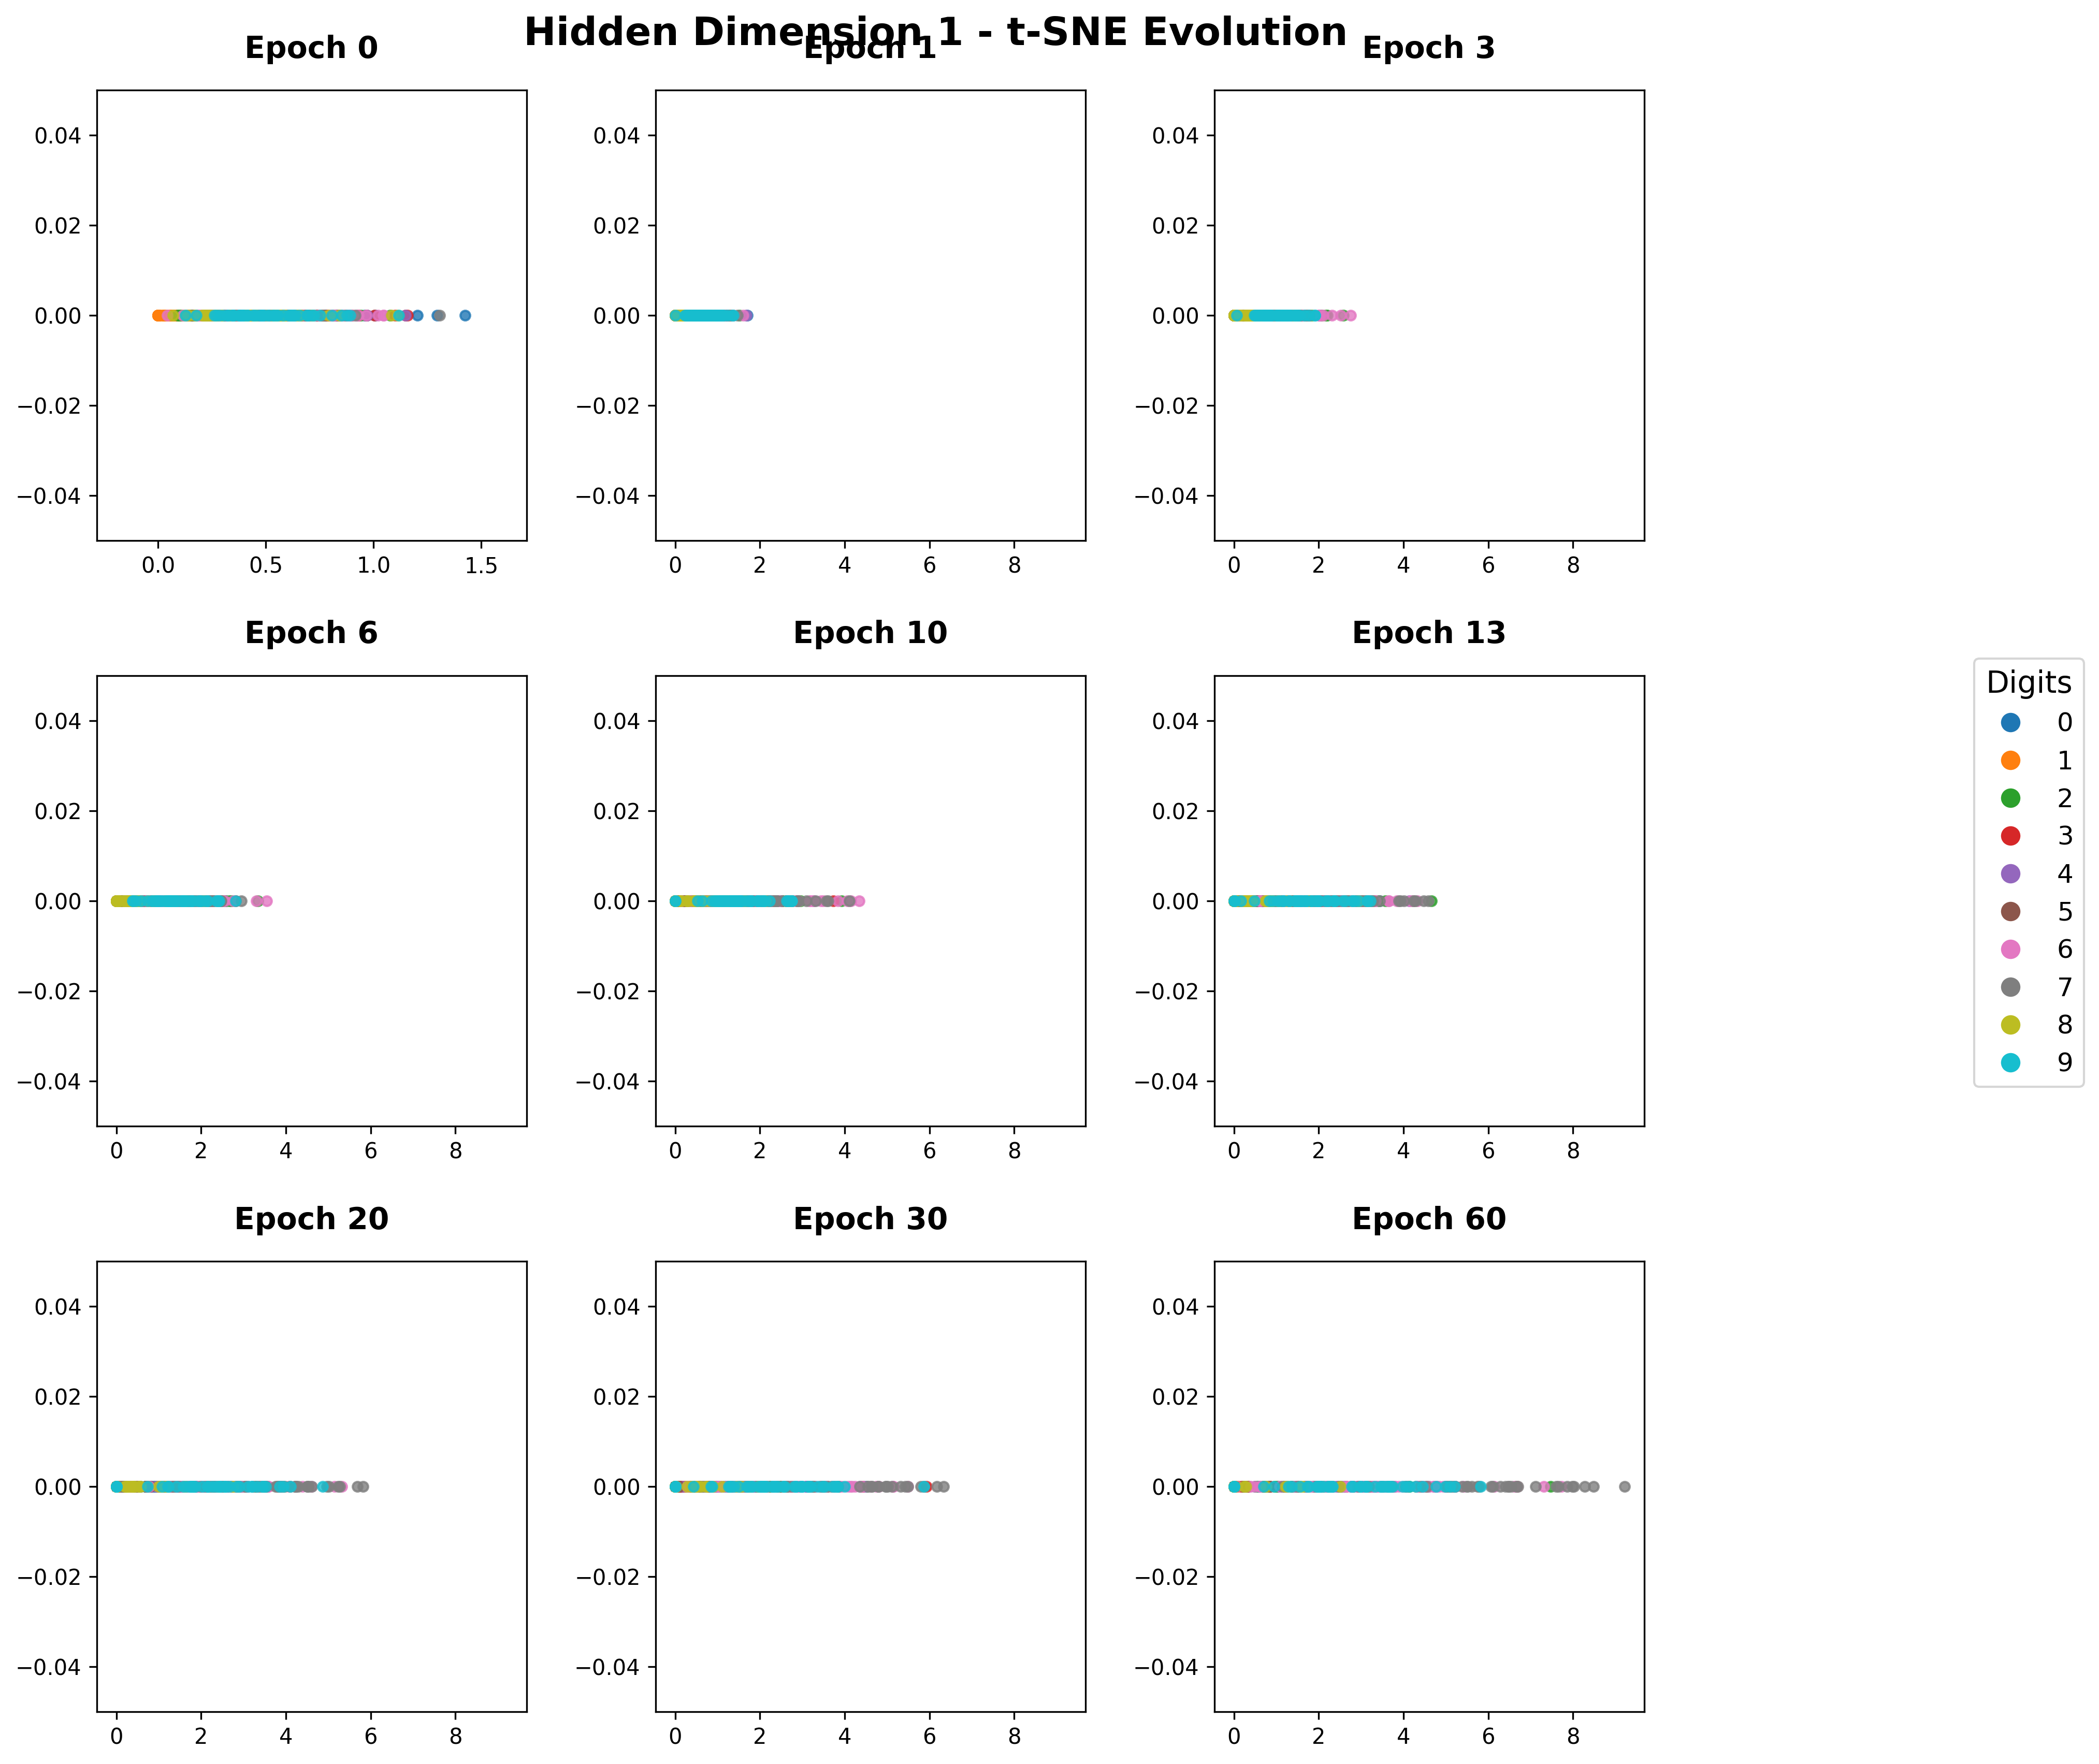
\includegraphics[width=0.8\textwidth]{../images/pa/tsne_evolution_hidden_1.png}
    \caption{隐层神经元数为1时的t-SNE可视化演化}
    \label{fig:1}
\end{figure}
\begin{figure}[H]
    \centering
    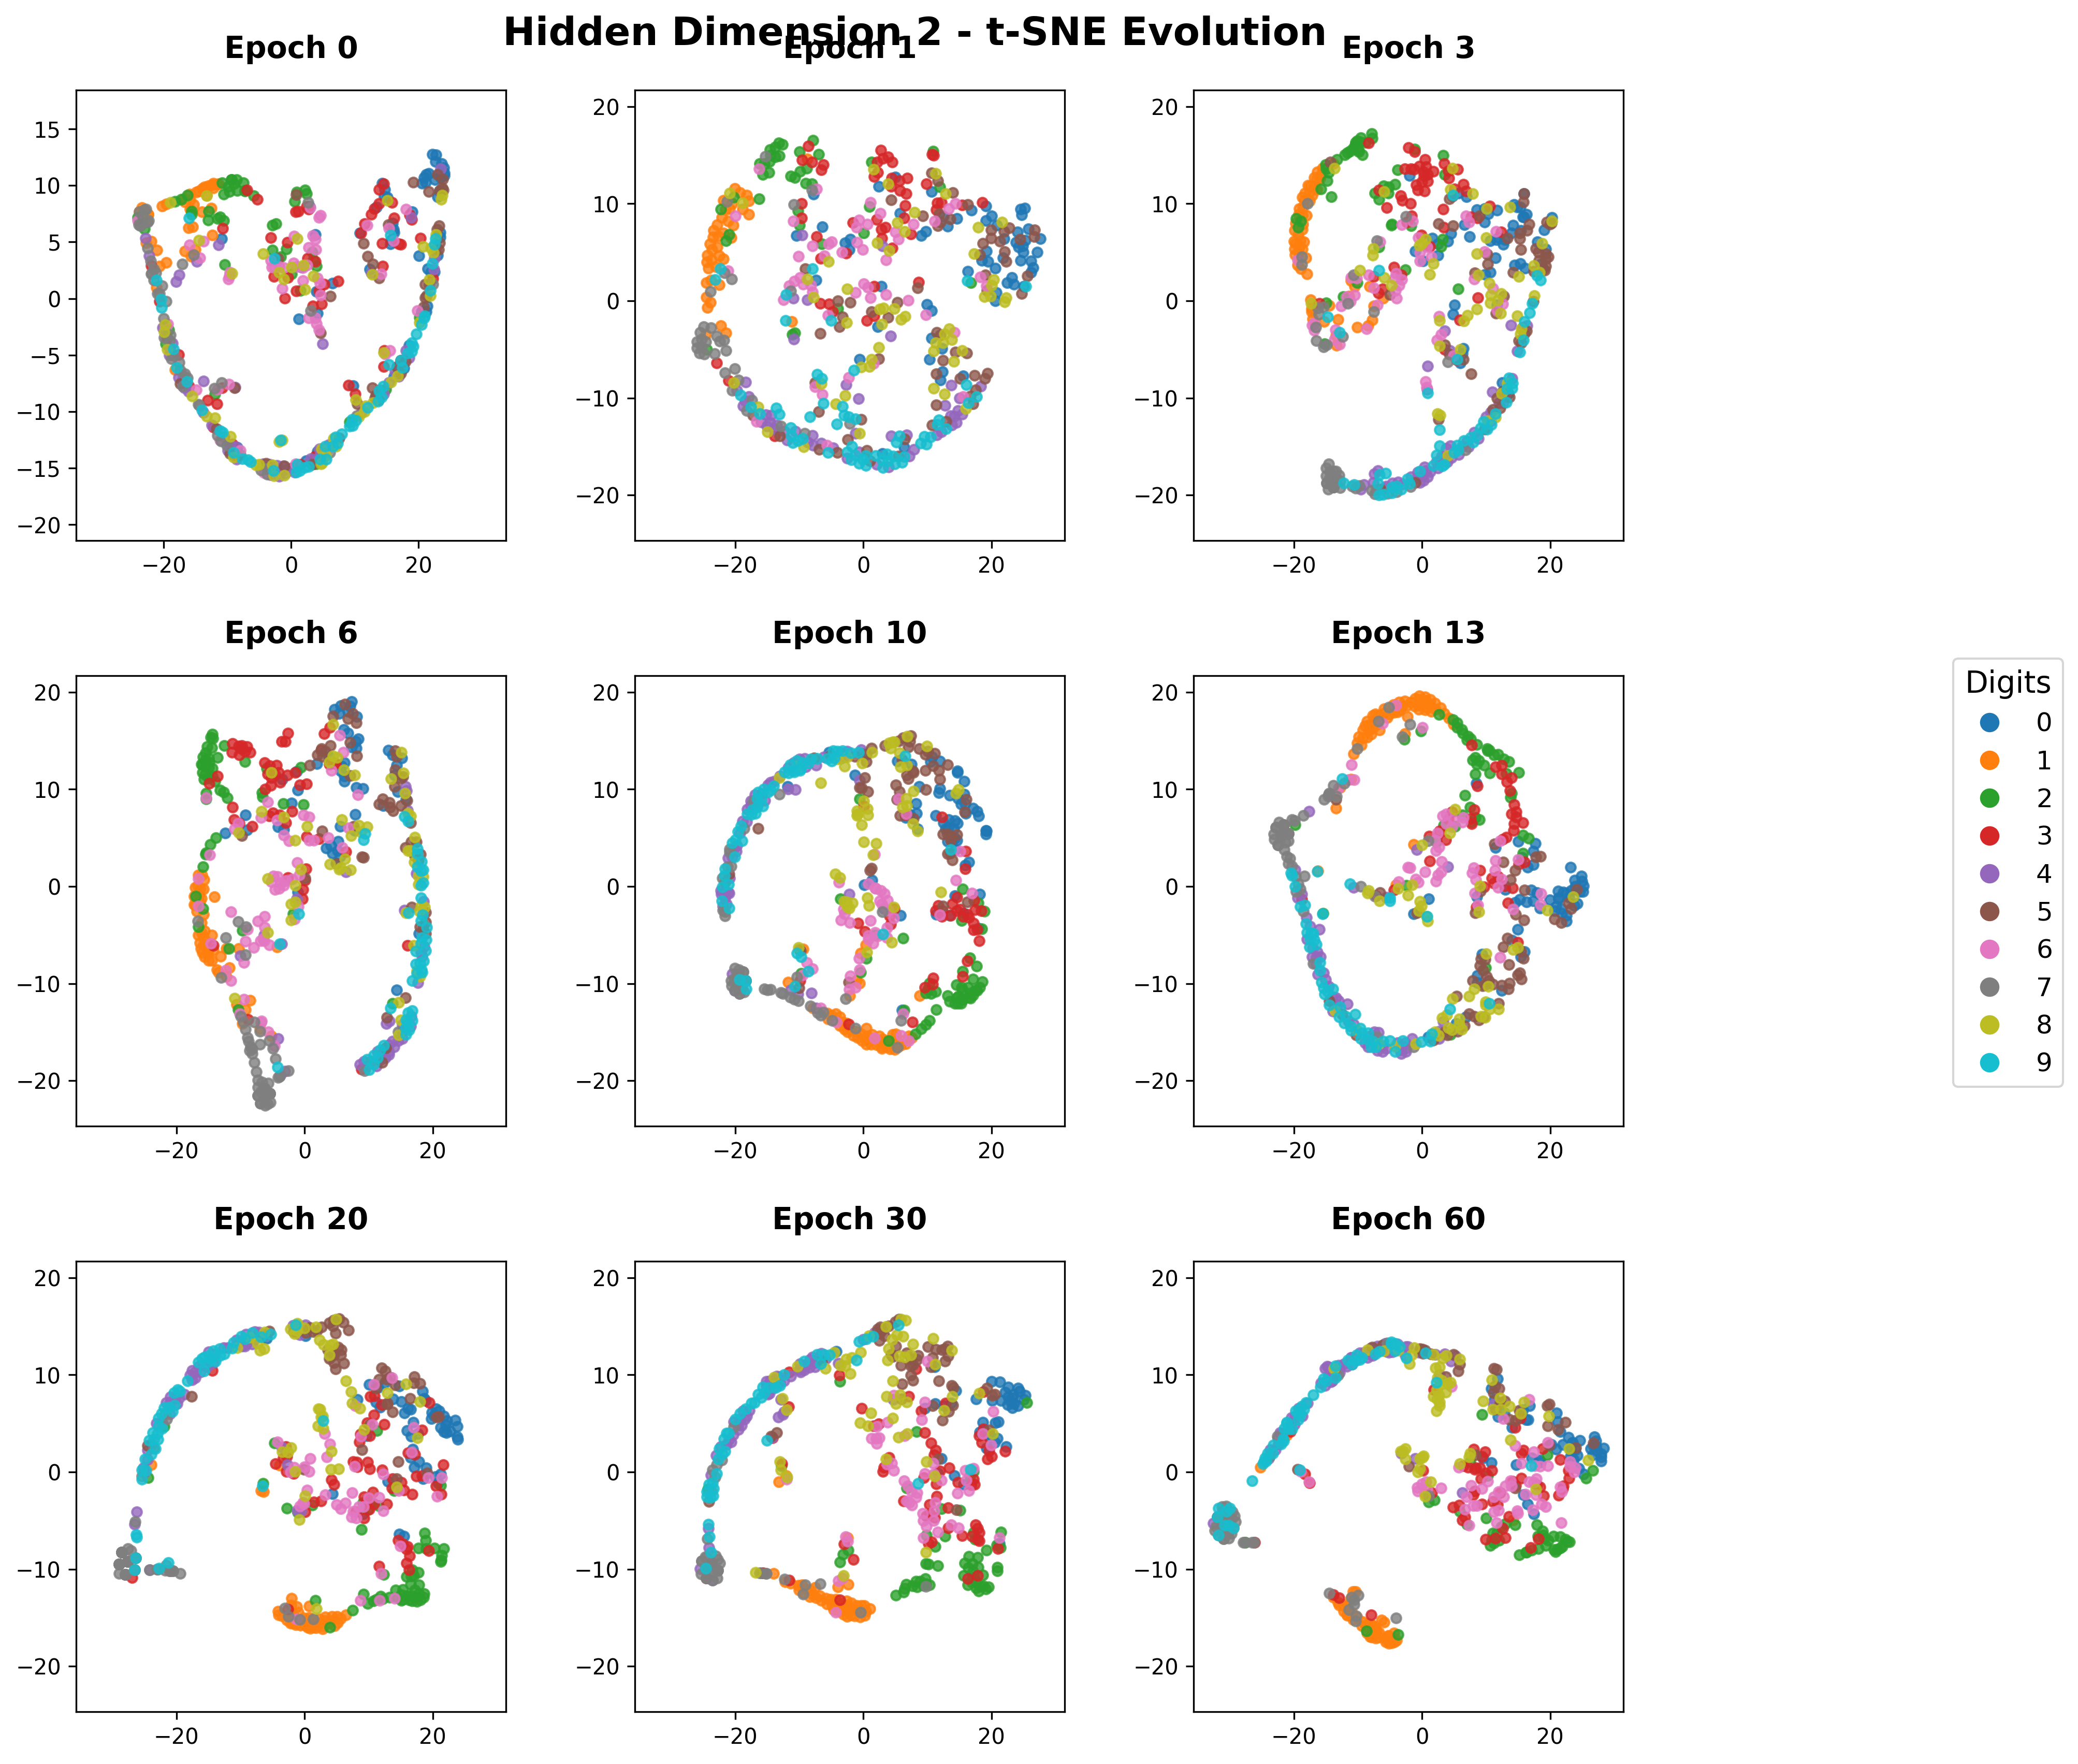
\includegraphics[width=0.8\textwidth]{../images/pa/tsne_evolution_hidden_2.png}
    \caption{隐层神经元数为2时的t-SNE可视化演化}
    \label{fig:2}
\end{figure}
\begin{figure}[H]
    \centering
    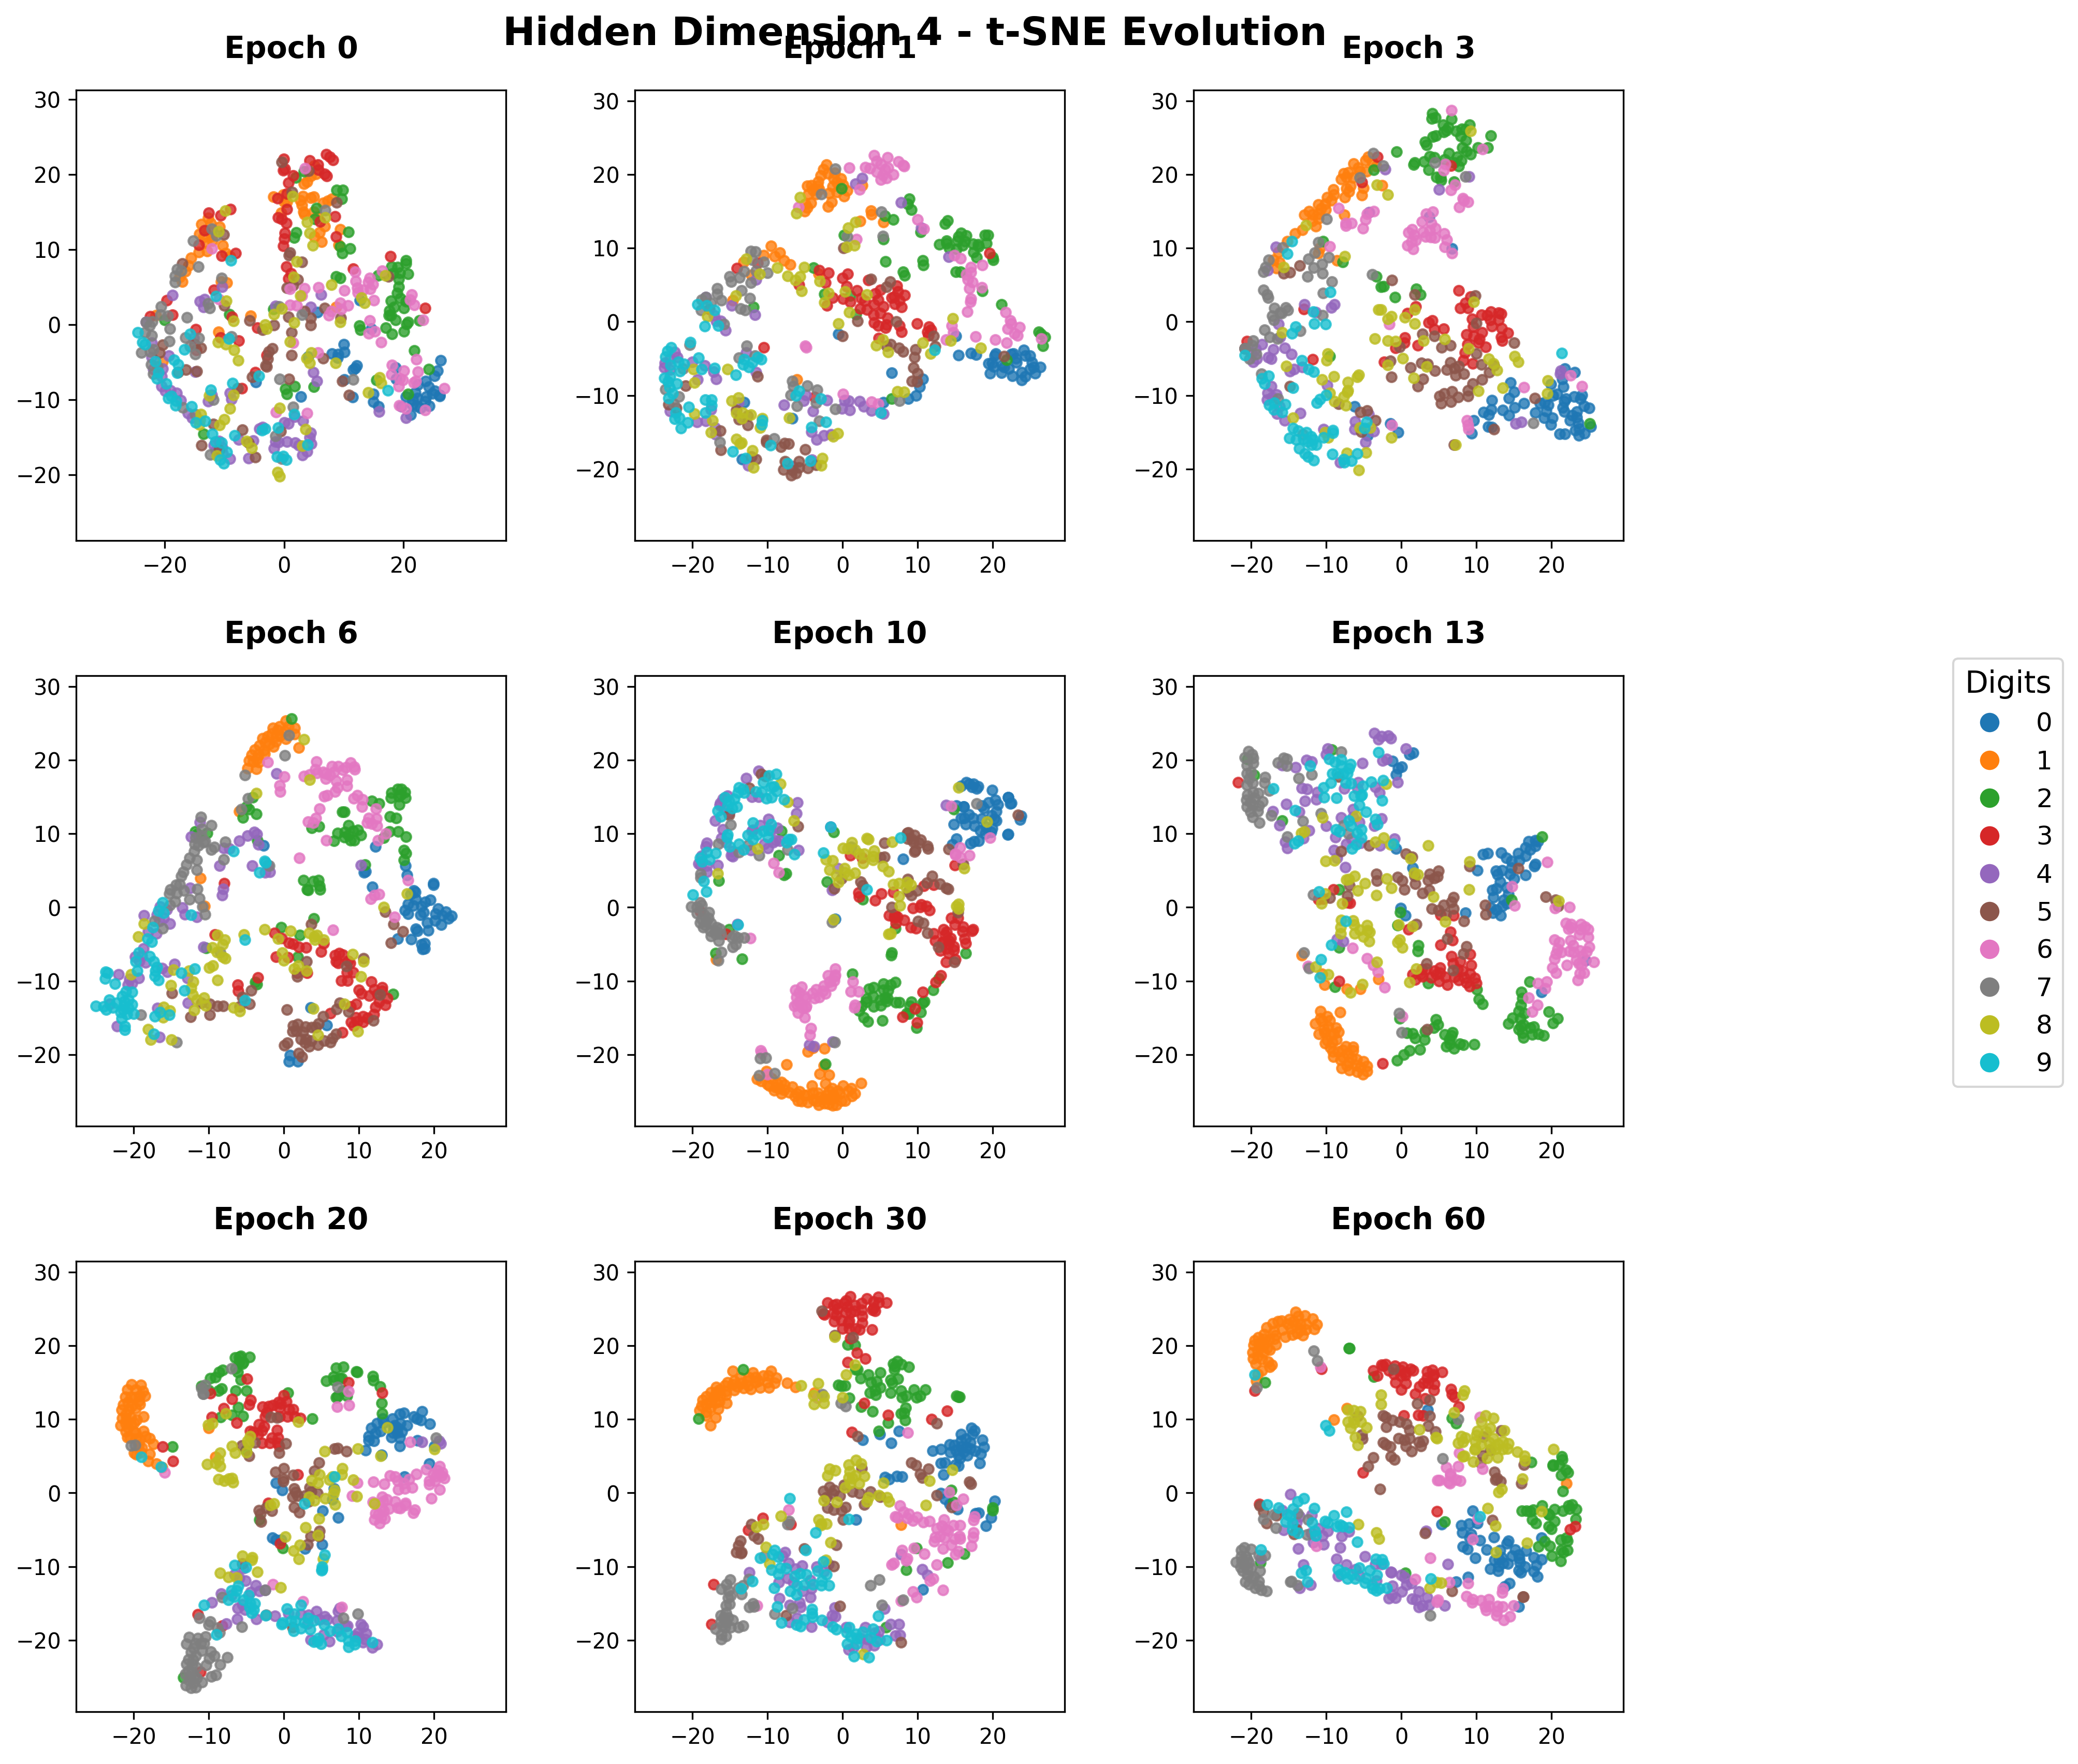
\includegraphics[width=0.8\textwidth]{../images/pa/tsne_evolution_hidden_4.png}
    \caption{隐层神经元数为4时的t-SNE可视化演化}
    \label{fig:4}
\end{figure}
\begin{figure}[H]
    \centering
    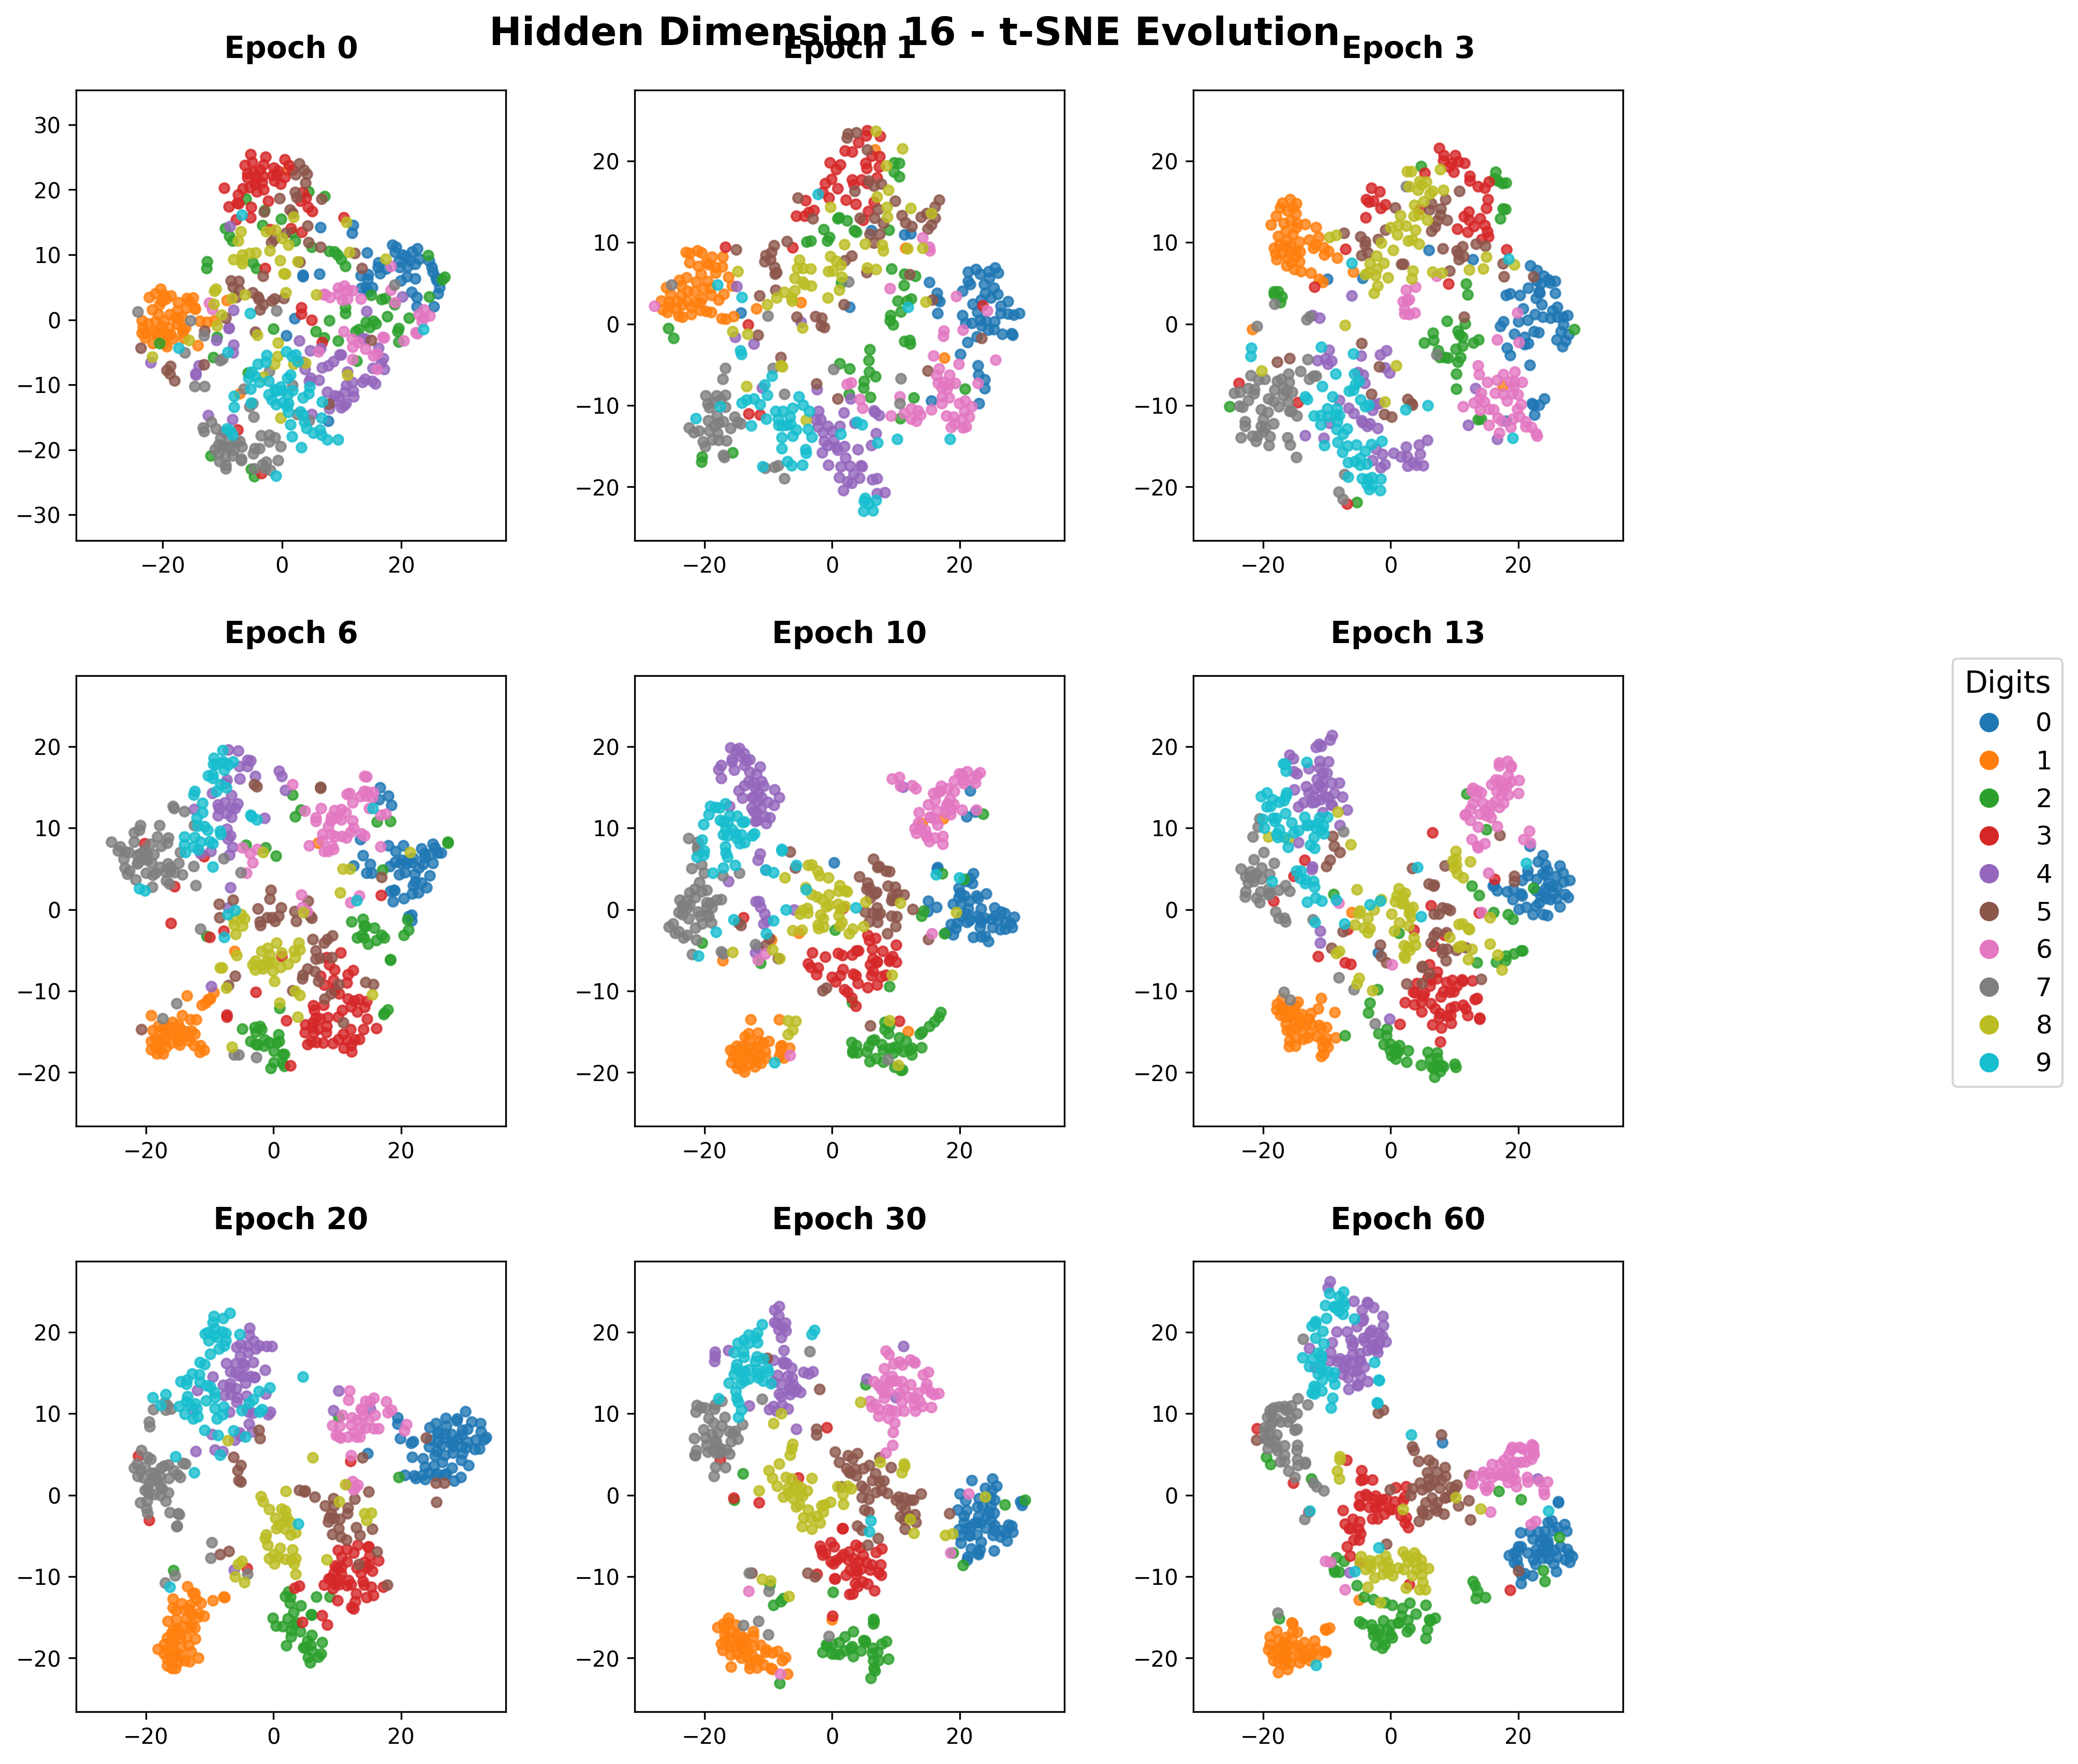
\includegraphics[width=0.8\textwidth]{../images/pa/tsne_evolution_hidden_16.png}
    \caption{隐层神经元数为16时的t-SNE可视化演化}
    \label{fig:16}
\end{figure}
\begin{figure}[H]
    \centering
    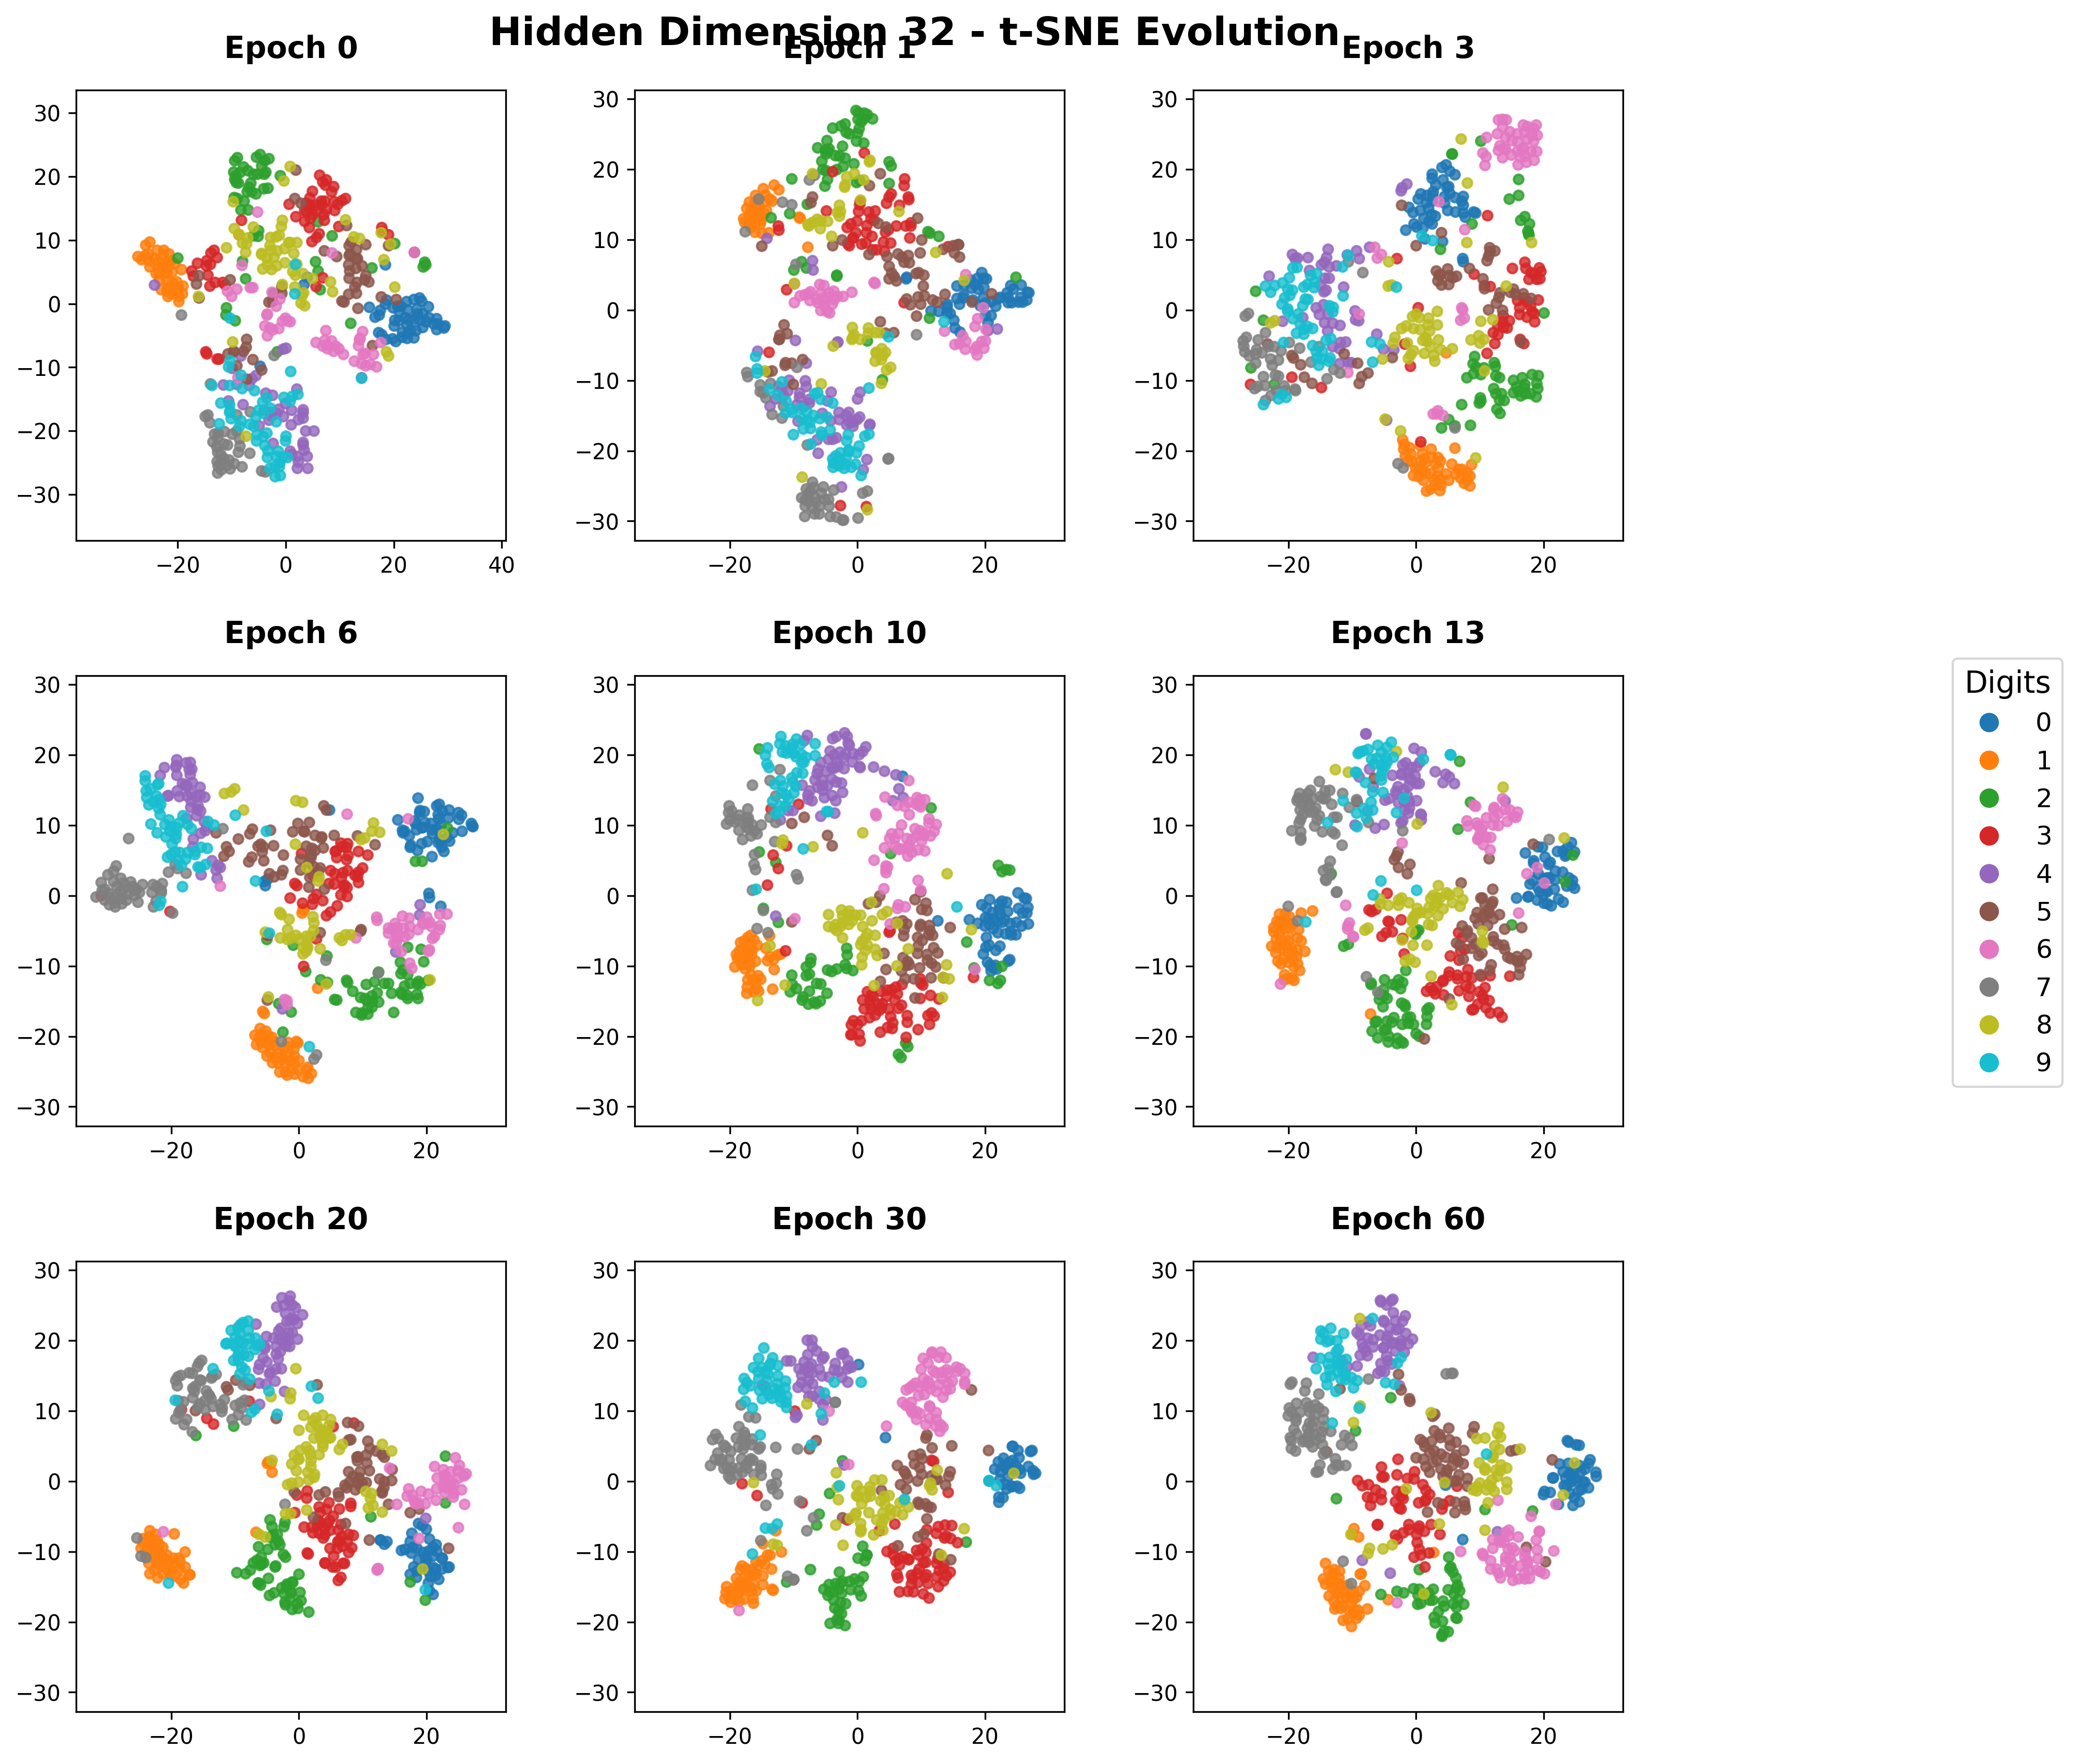
\includegraphics[width=0.8\textwidth]{../images/pa/tsne_evolution_hidden_32.png}
    \caption{隐层神经元数为32时的t-SNE可视化演化}
    \label{fig:32}
\end{figure}
\begin{figure}[H]
    \centering
    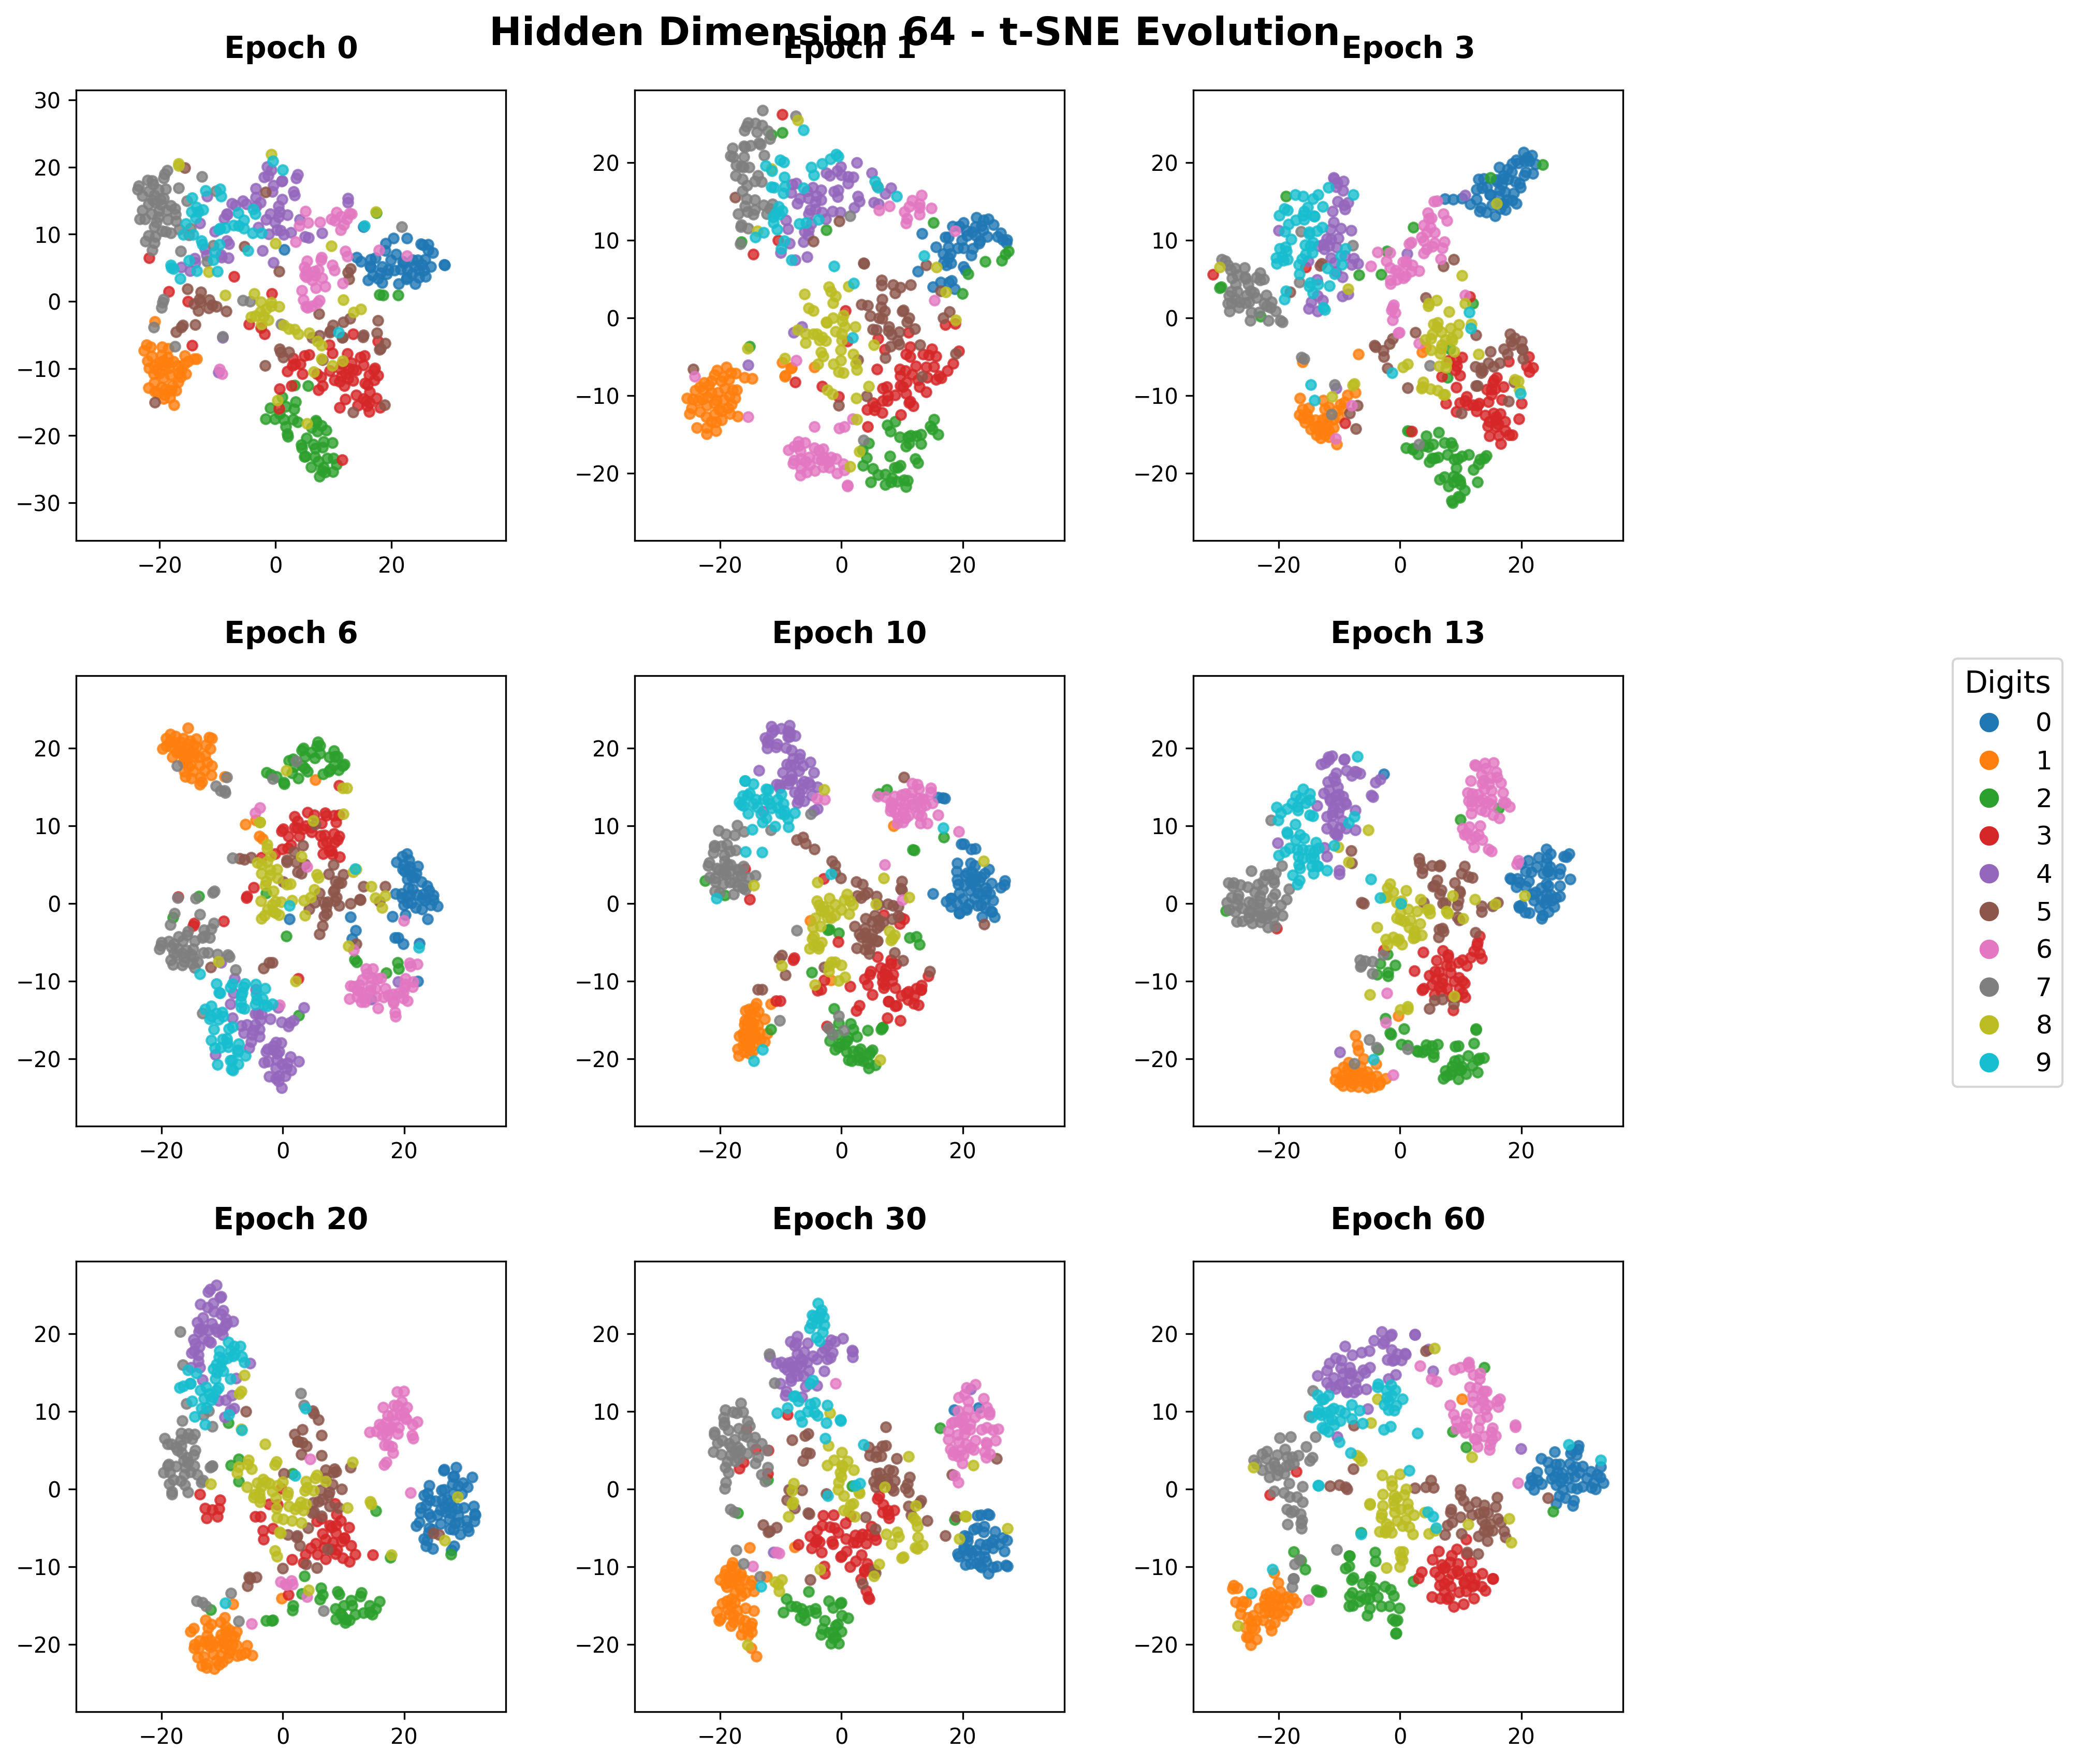
\includegraphics[width=0.8\textwidth]{../images/pa/tsne_evolution_hidden_64.png}
    \caption{隐层神经元数为64时的t-SNE可视化演化}
    \label{fig:64}
\end{figure}
\begin{figure}[H]
    \centering
    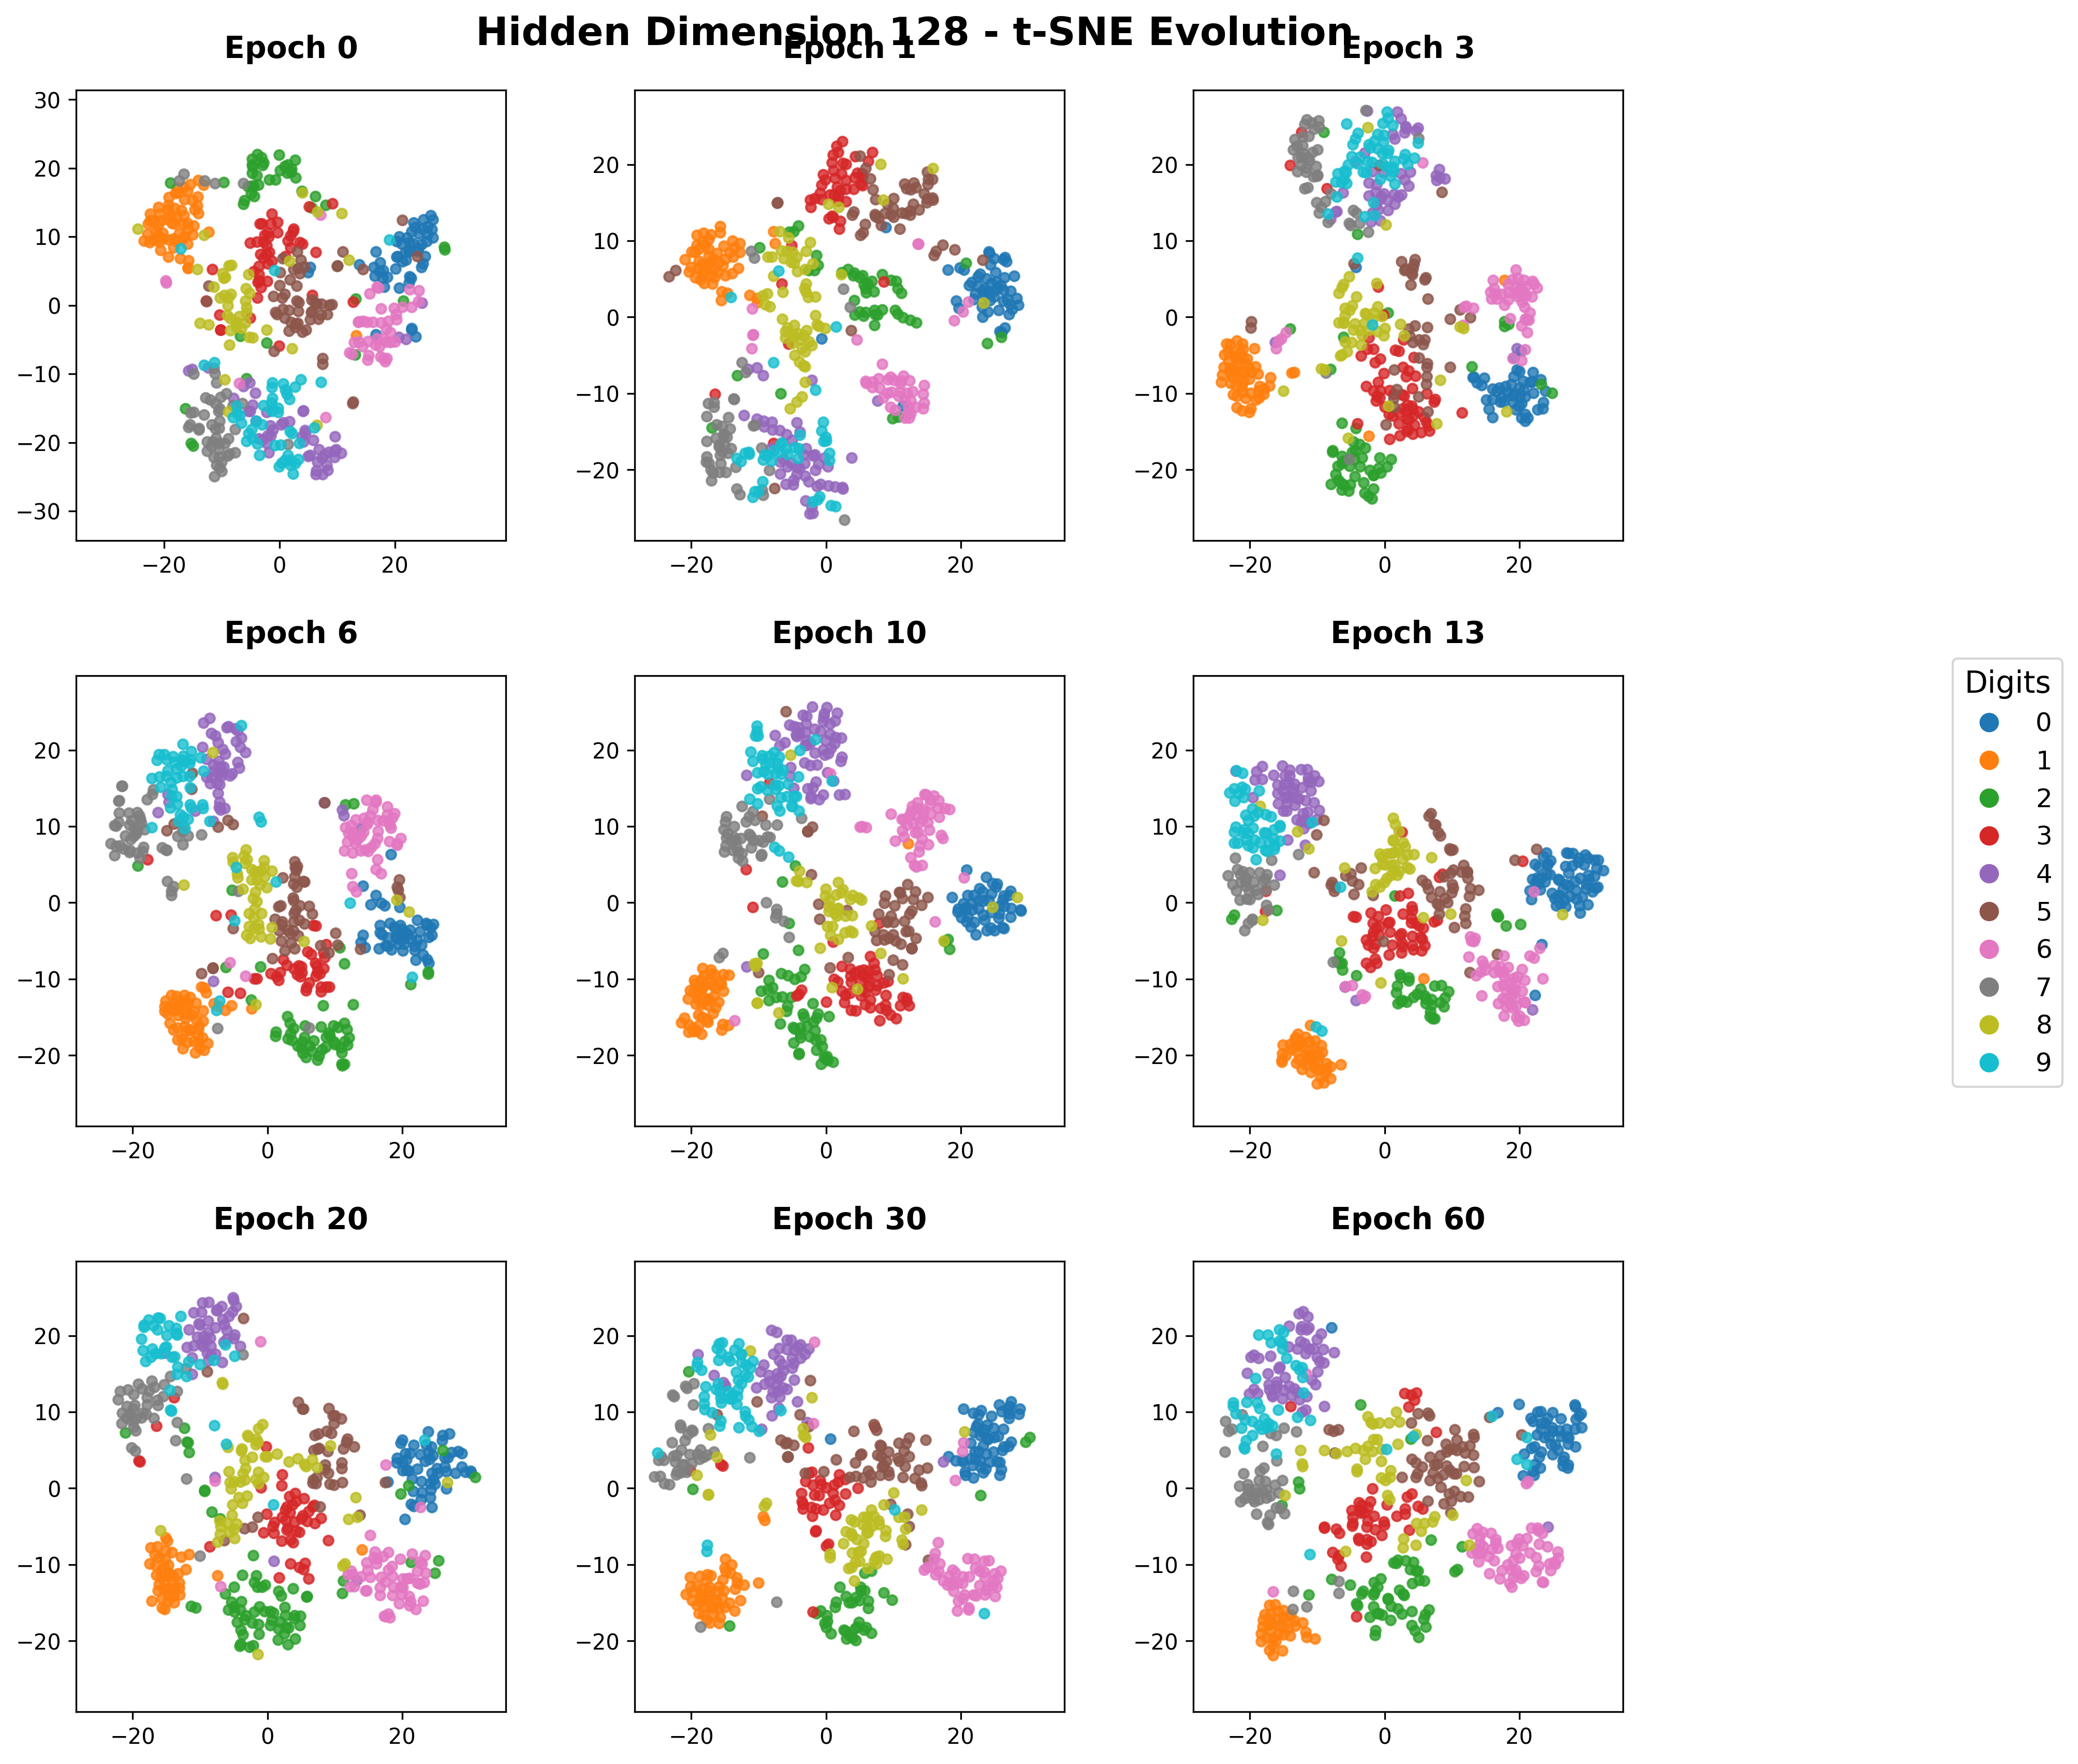
\includegraphics[width=0.8\textwidth]{../images/pa/tsne_evolution_hidden_128.png}
    \caption{隐层神经元数为128时的t-SNE可视化演化}
    \label{fig:128}
\end{figure}
\begin{figure}[H]
    \centering
    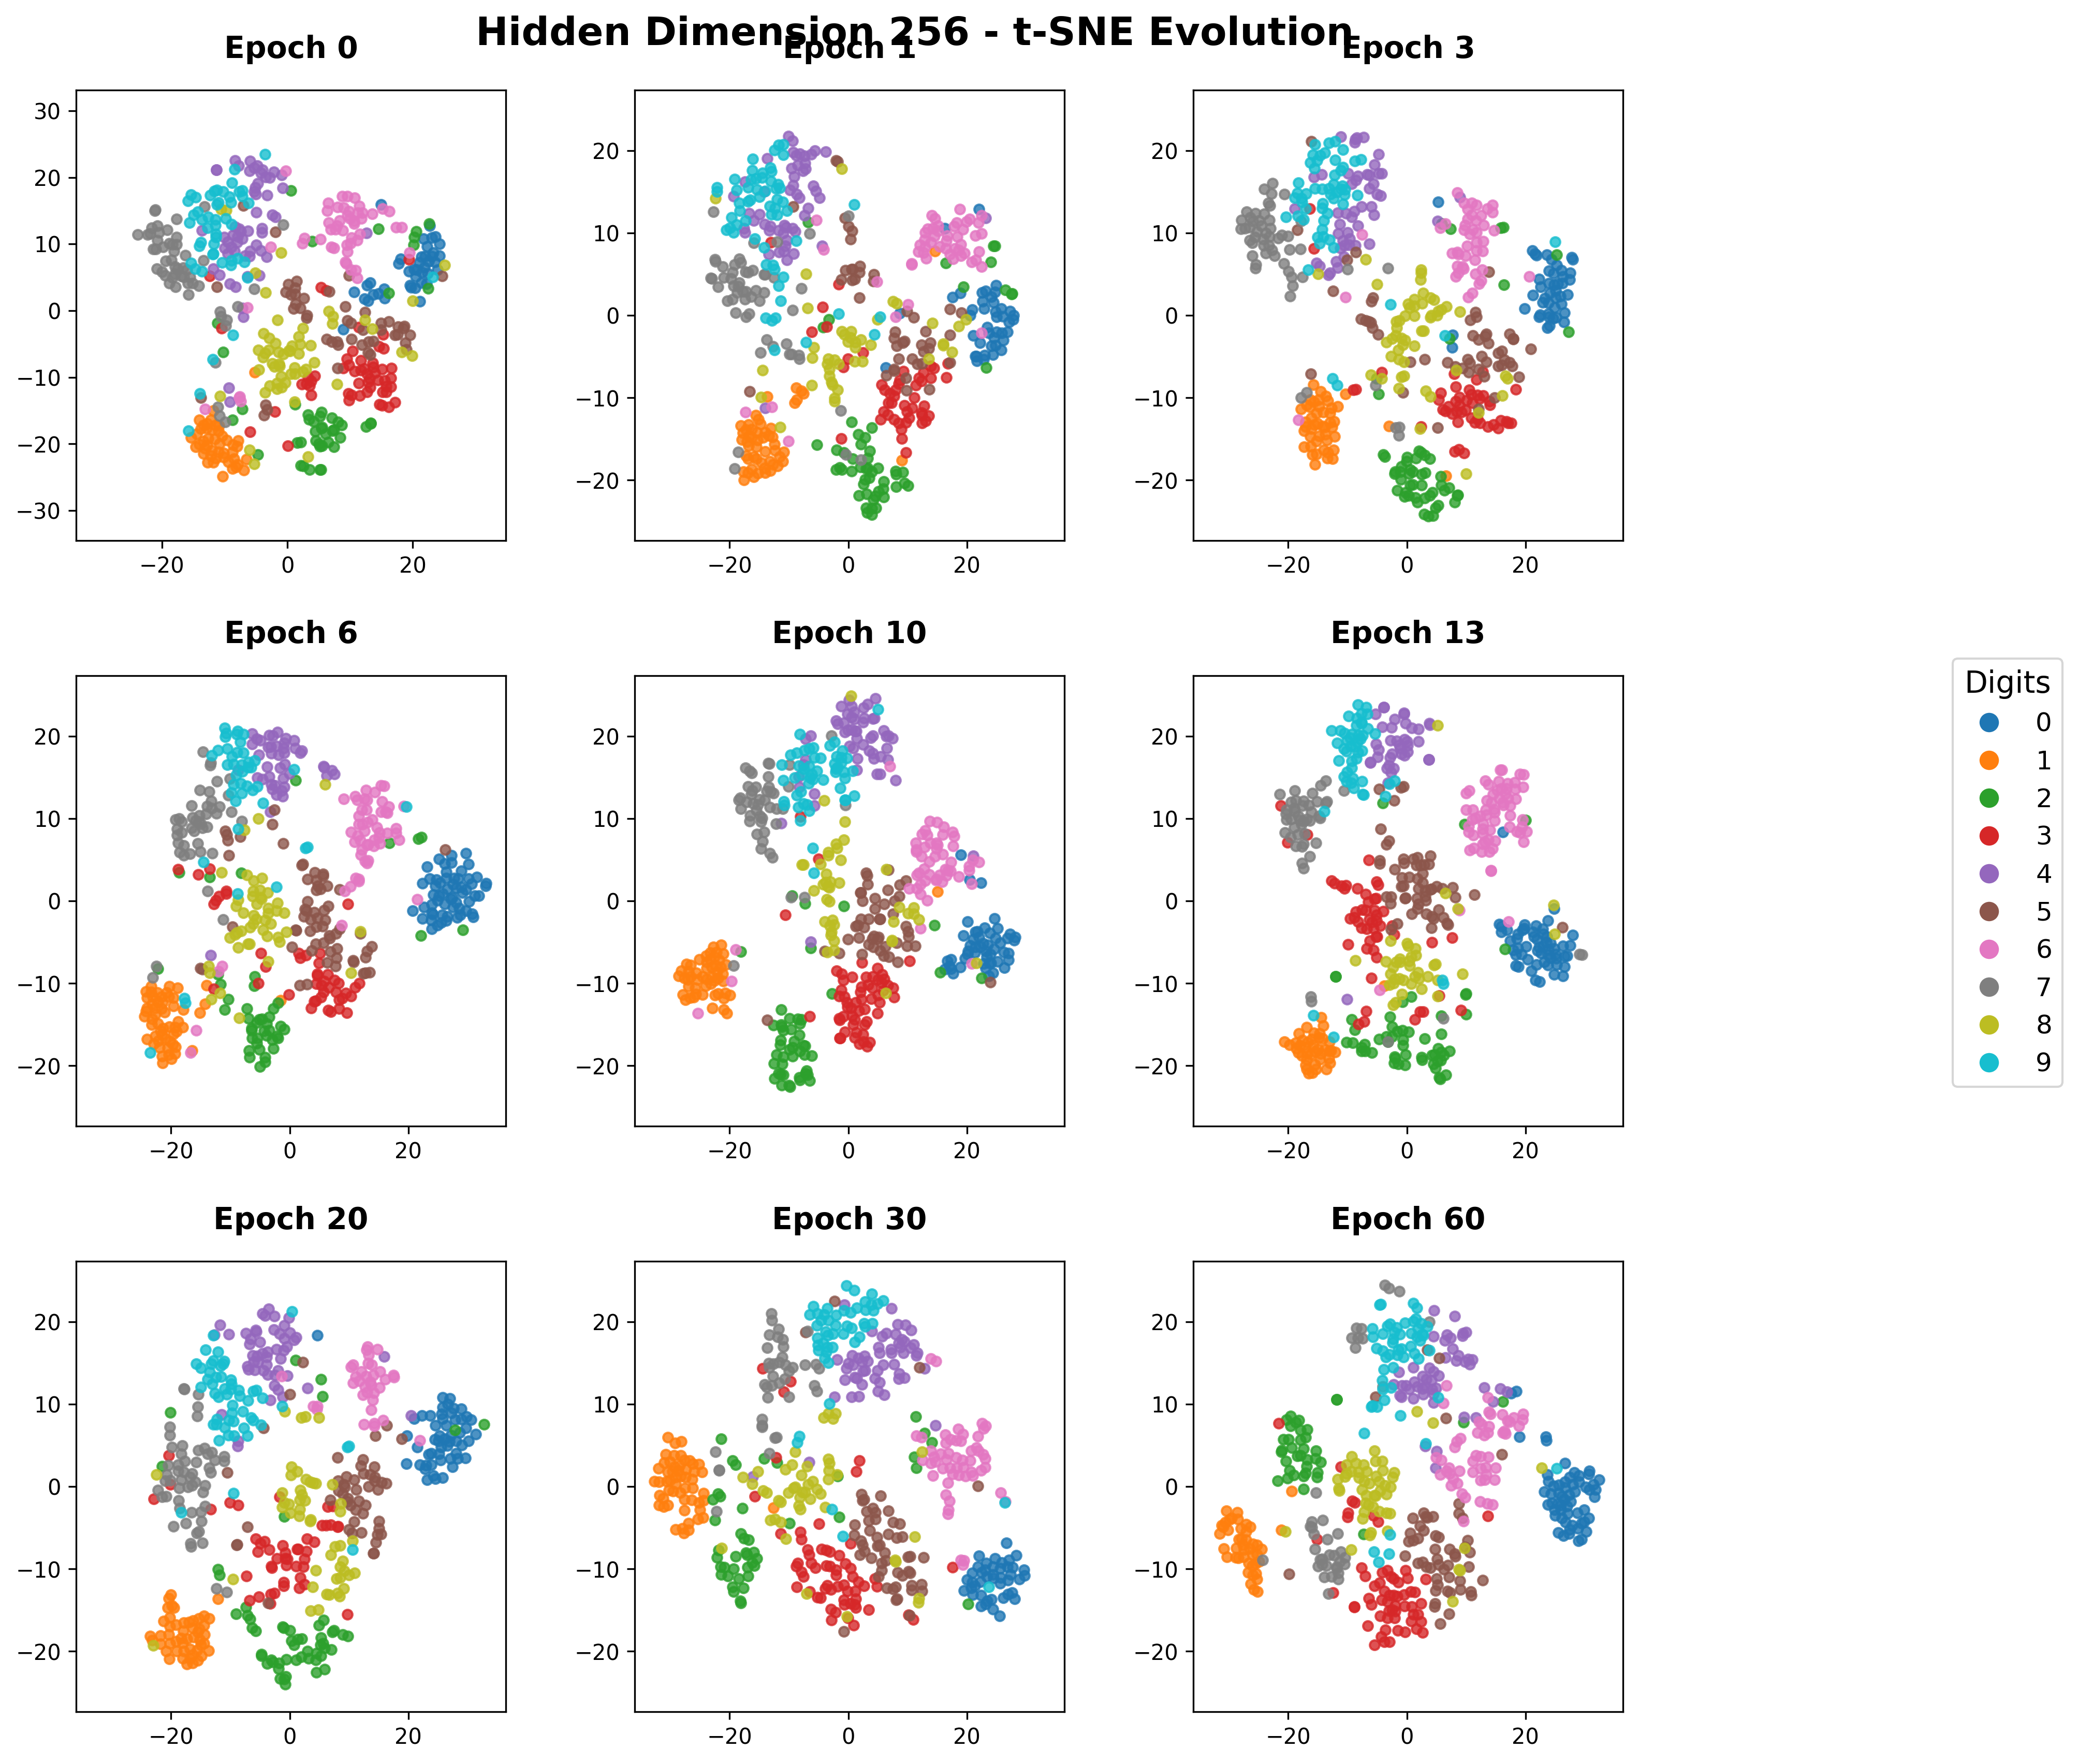
\includegraphics[width=0.8\textwidth]{../images/pa/tsne_evolution_hidden_256.png}
    \caption{隐层神经元数为256时的t-SNE可视化演化}
    \label{fig:256}
\end{figure}
\begin{figure}[H]
    \centering
    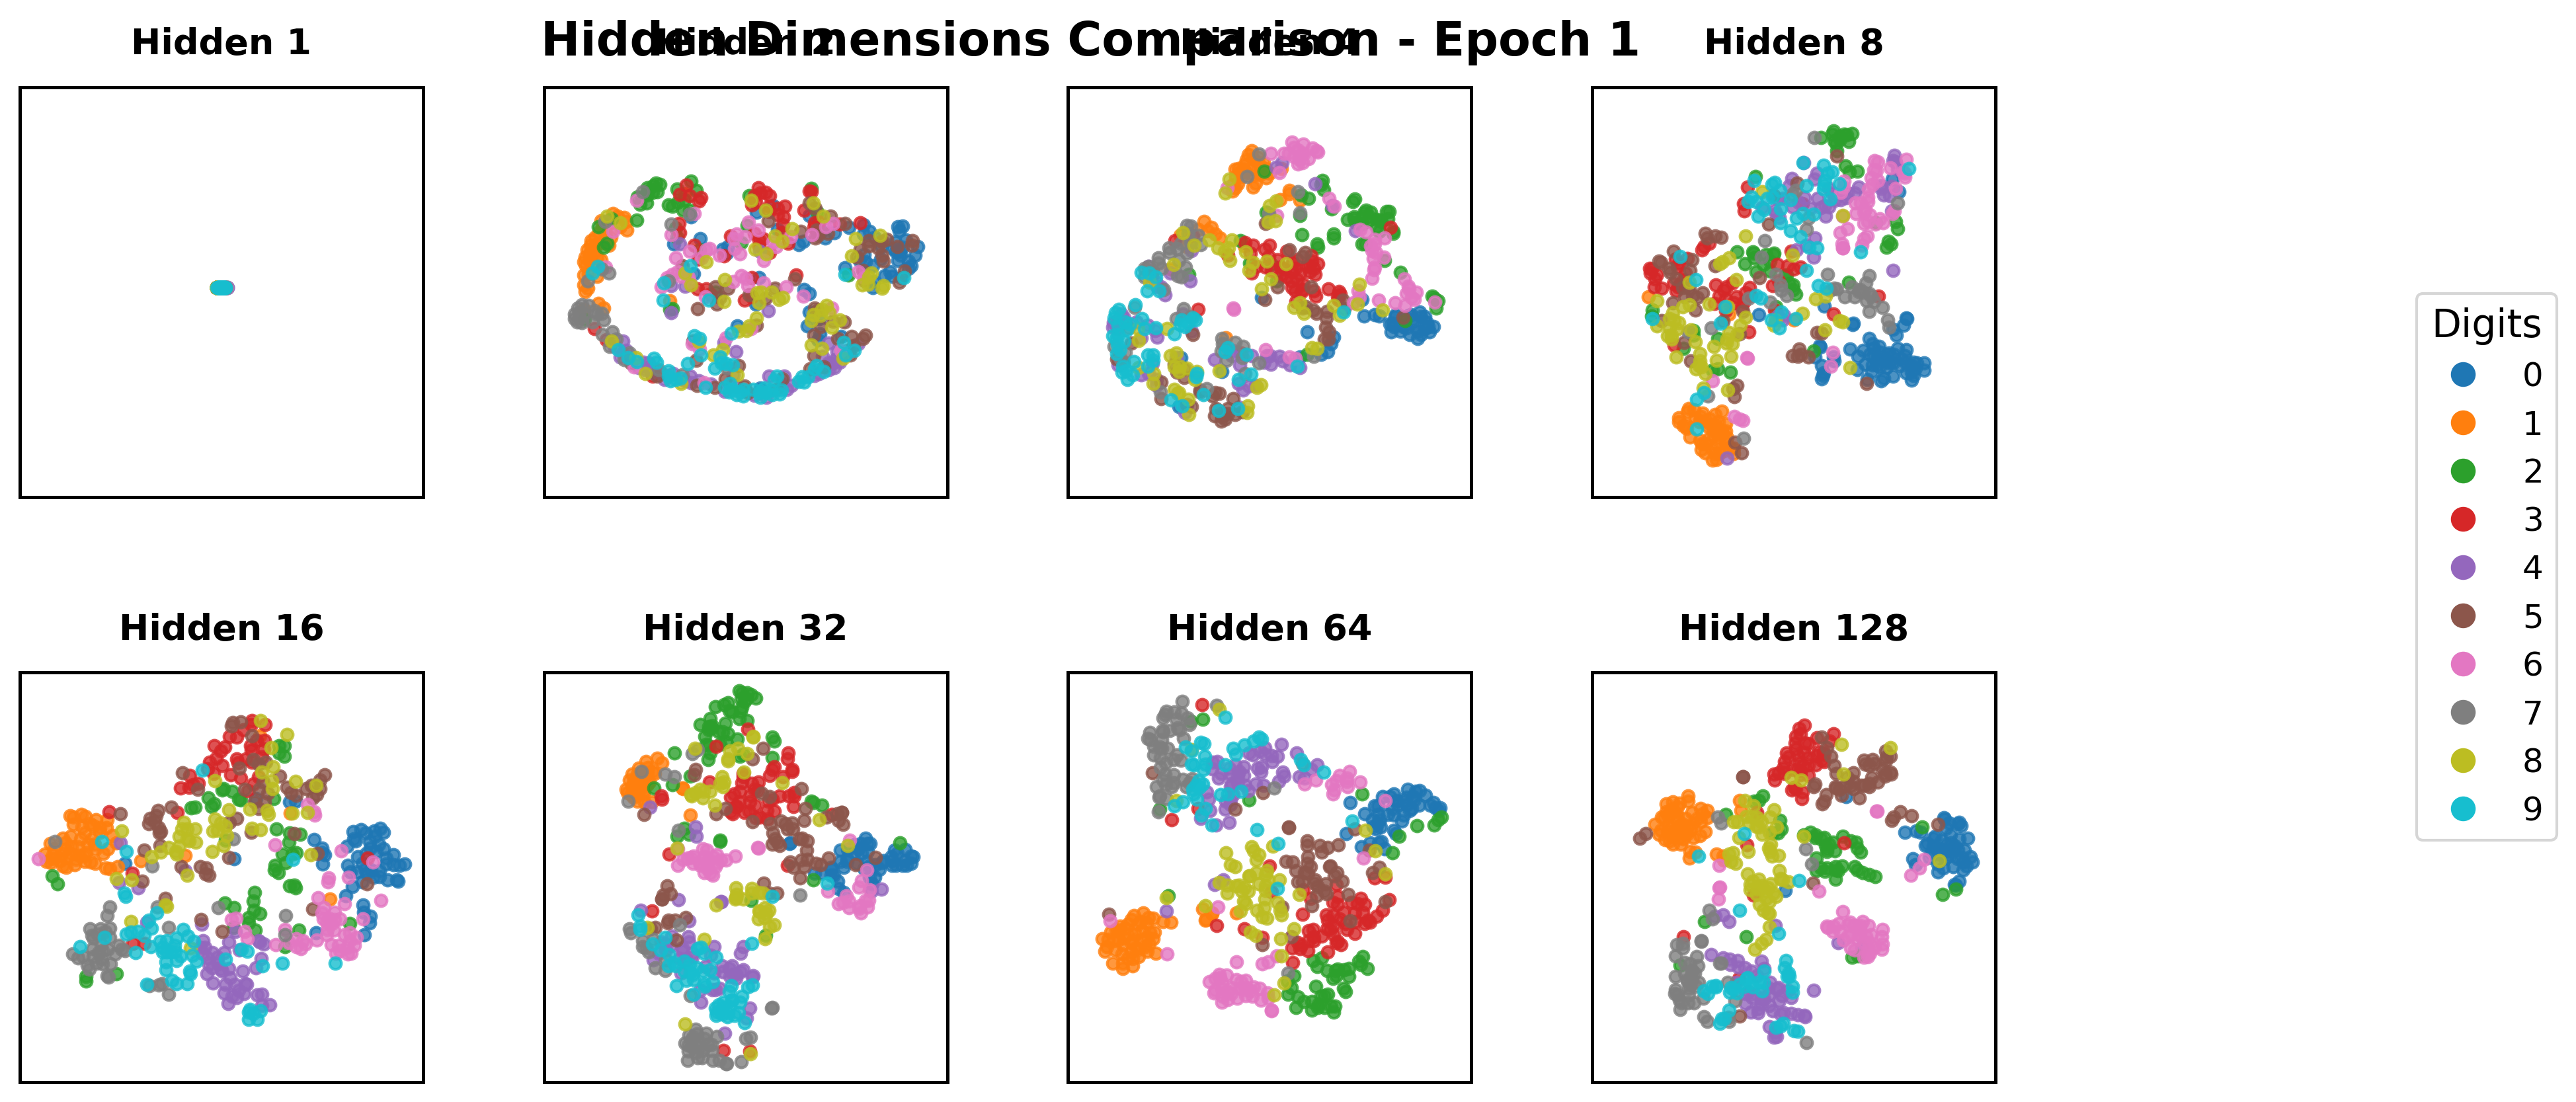
\includegraphics[width=0.8\textwidth]{../images/pa/tsne_comparison_epoch_1.png}
    \caption{t-SNE可视化对比(epoch=1)}
    \label{fig:11}
\end{figure}

\section{冻结实验结果}\label{sec:feature_extractor_classifier}
\begin{figure}[H]
    \centering
    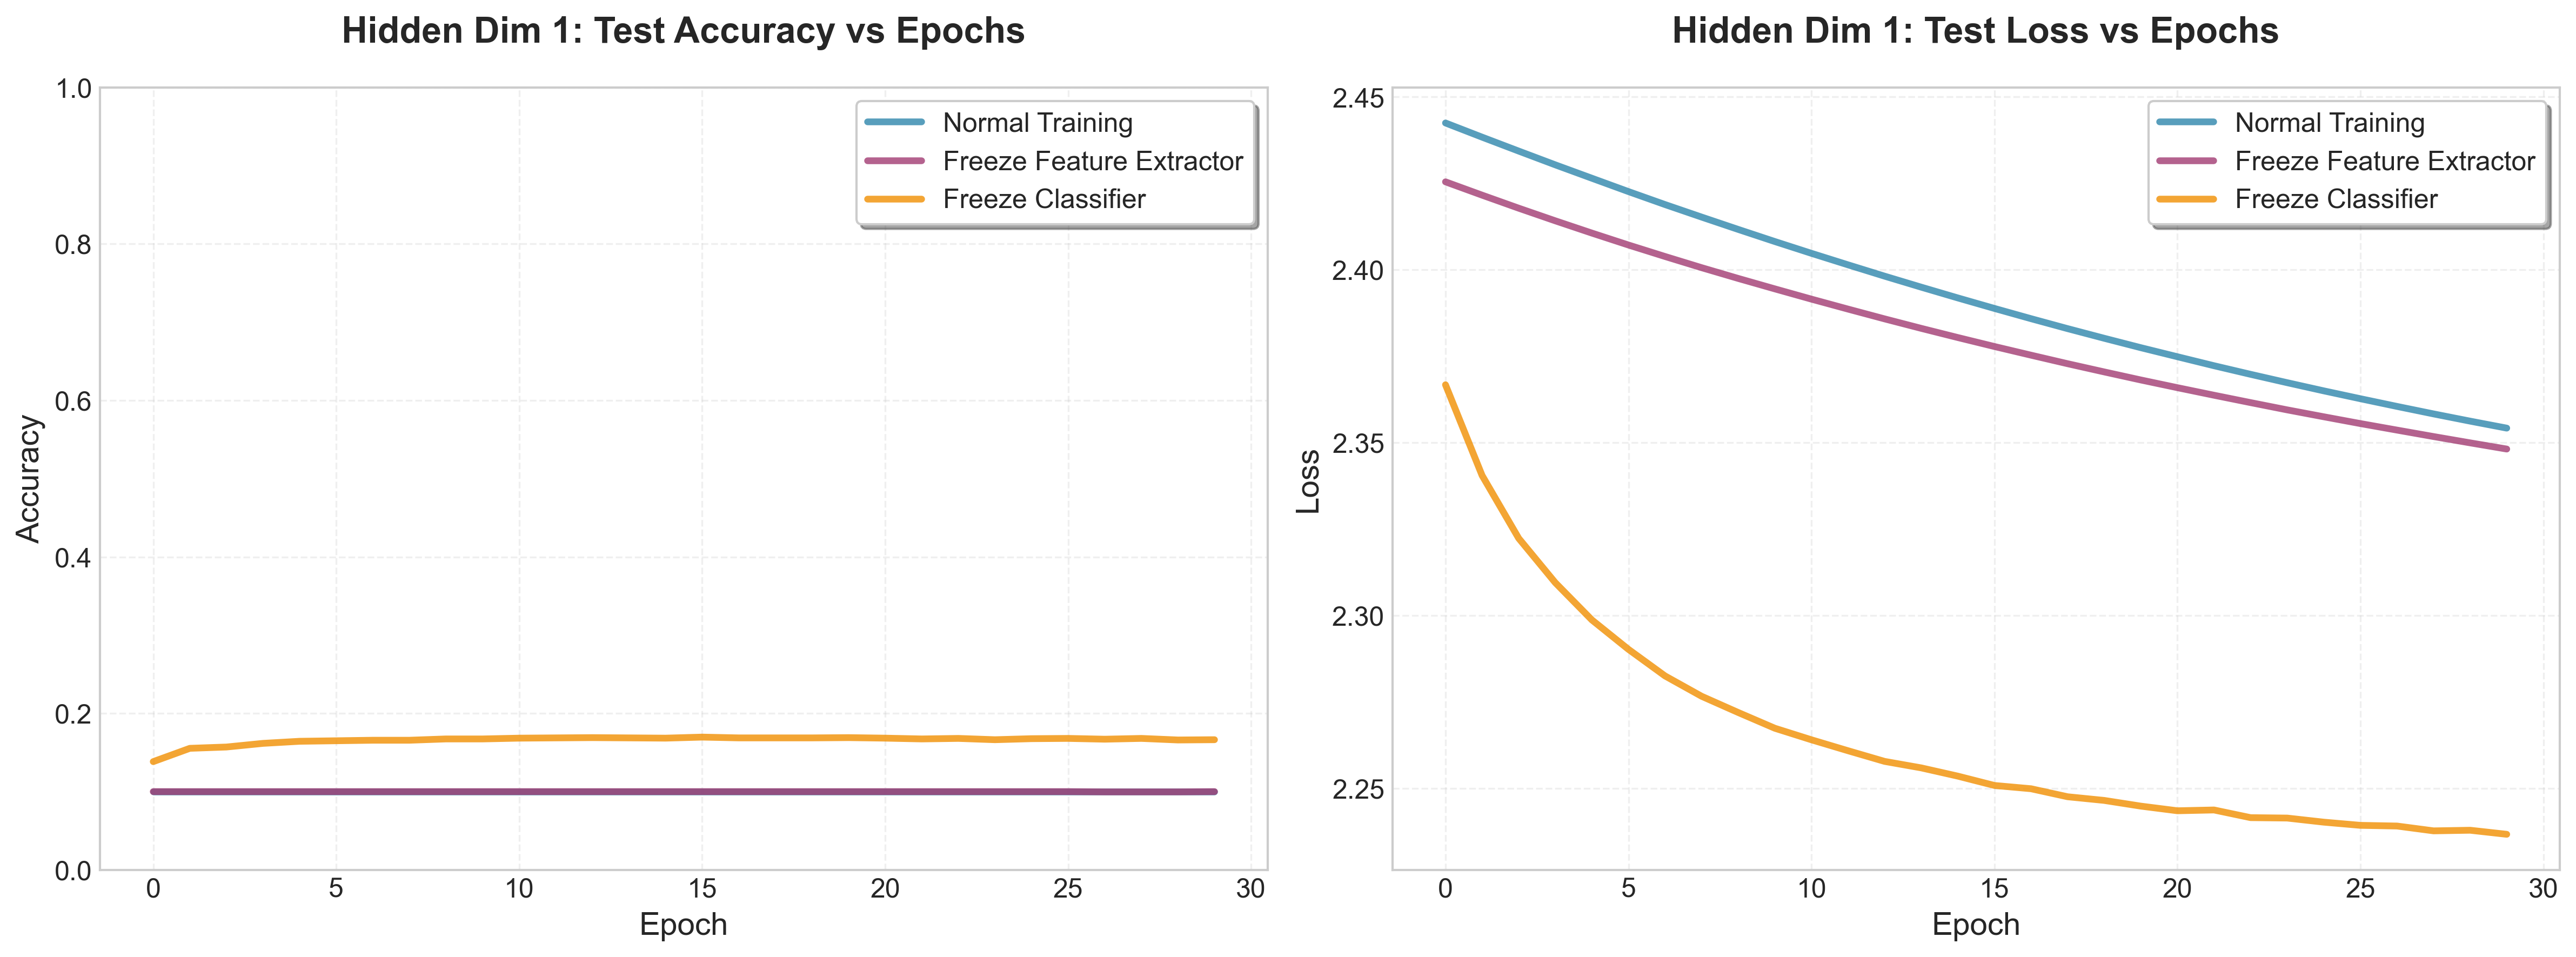
\includegraphics[width=0.8\textwidth]{../images/dd/hidden_1_comparison.png}
    \caption{冻结实验结果对比(隐藏层神经元数为1)}
    \label{fig:hidden_1_comparison.png}
\end{figure}
\begin{figure}[H]
    \centering
    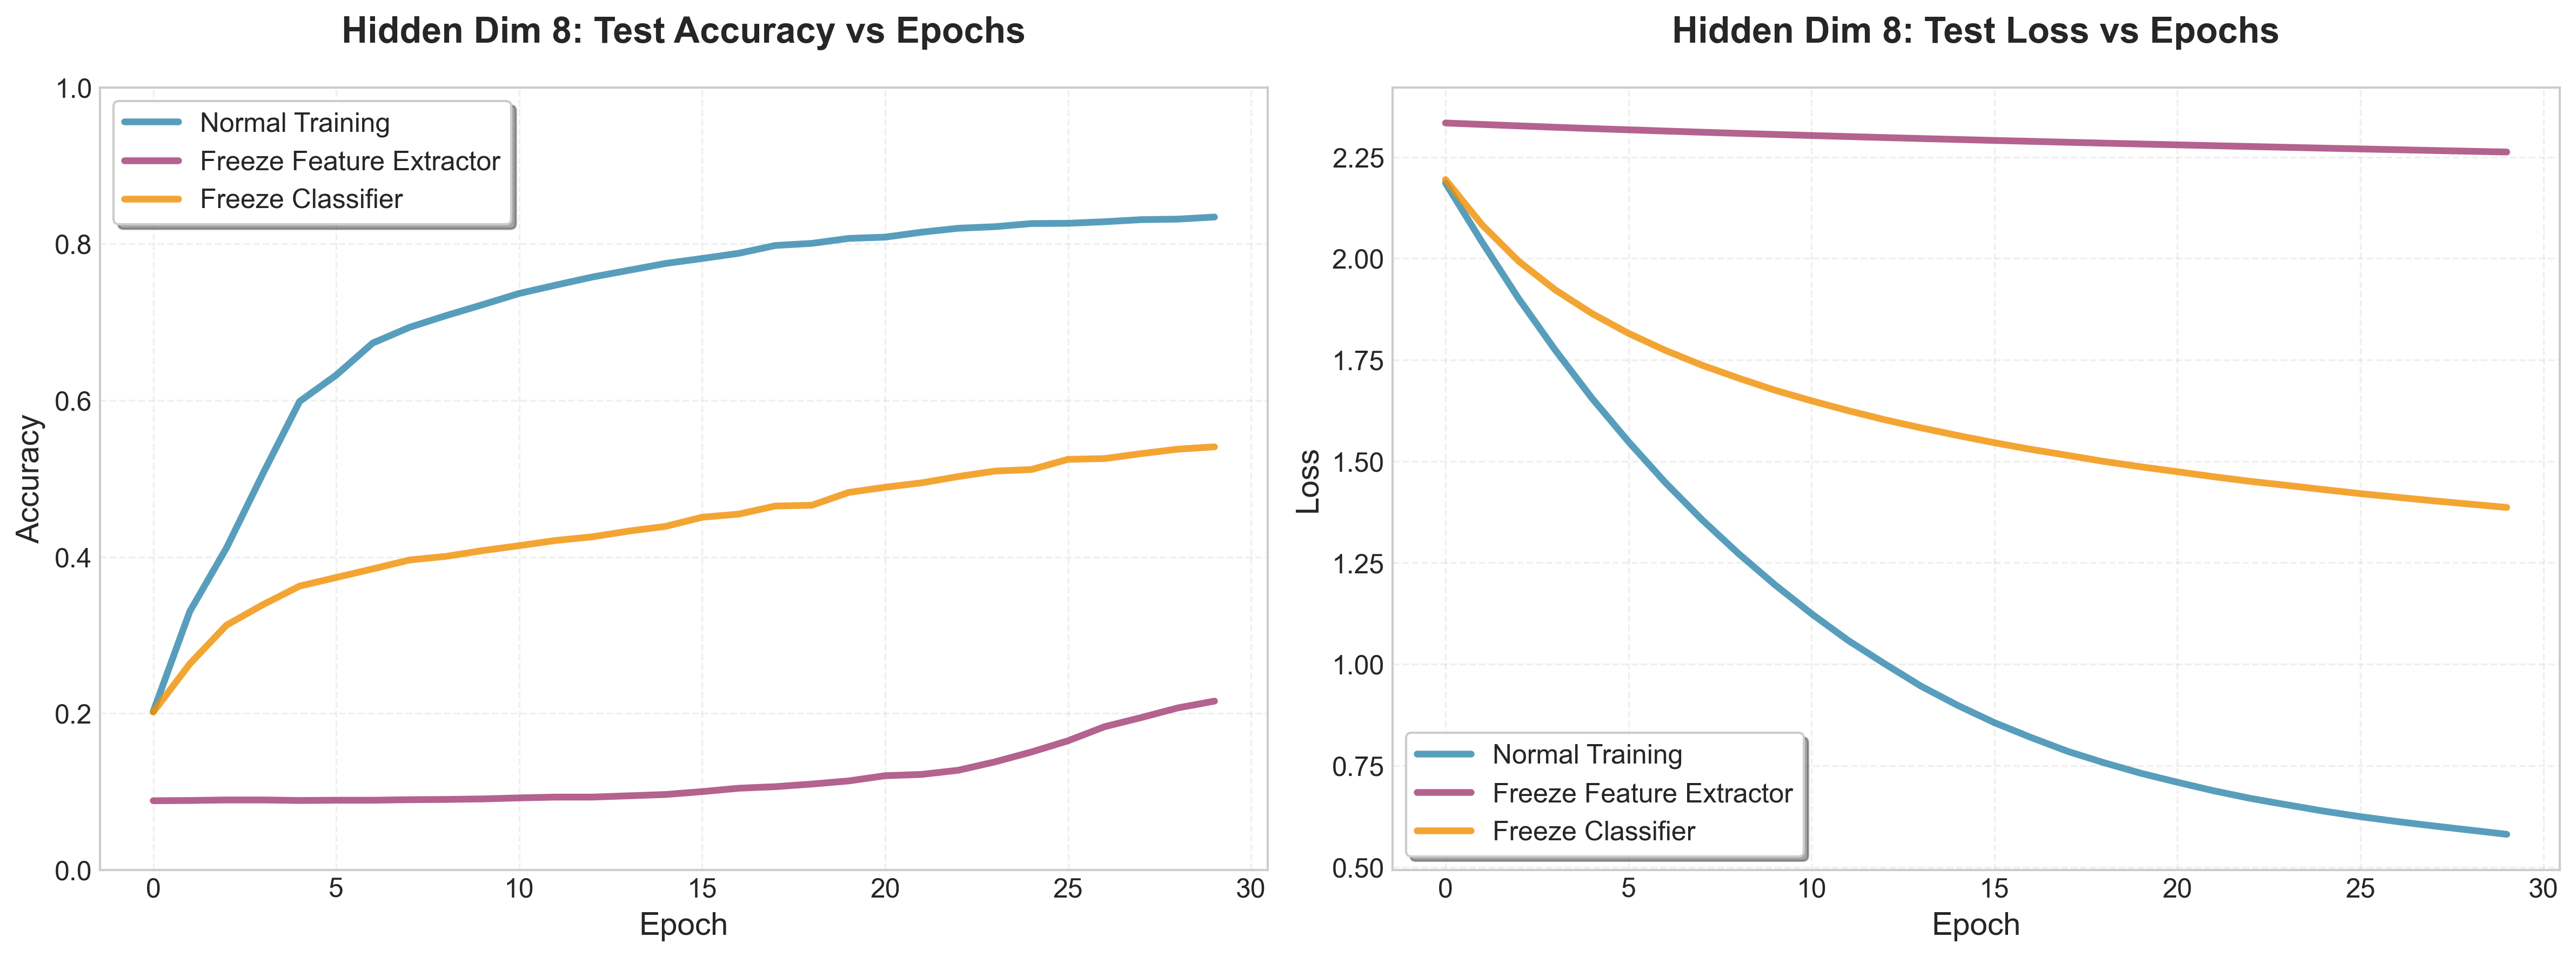
\includegraphics[width=0.8\textwidth]{../images/dd/hidden_8_comparison.png}
    \caption{冻结实验结果对比(隐藏层神经元数为8)}
    \label{fig:hidden_8_comparison.png}
\end{figure}
\begin{figure}[H]
    \centering
    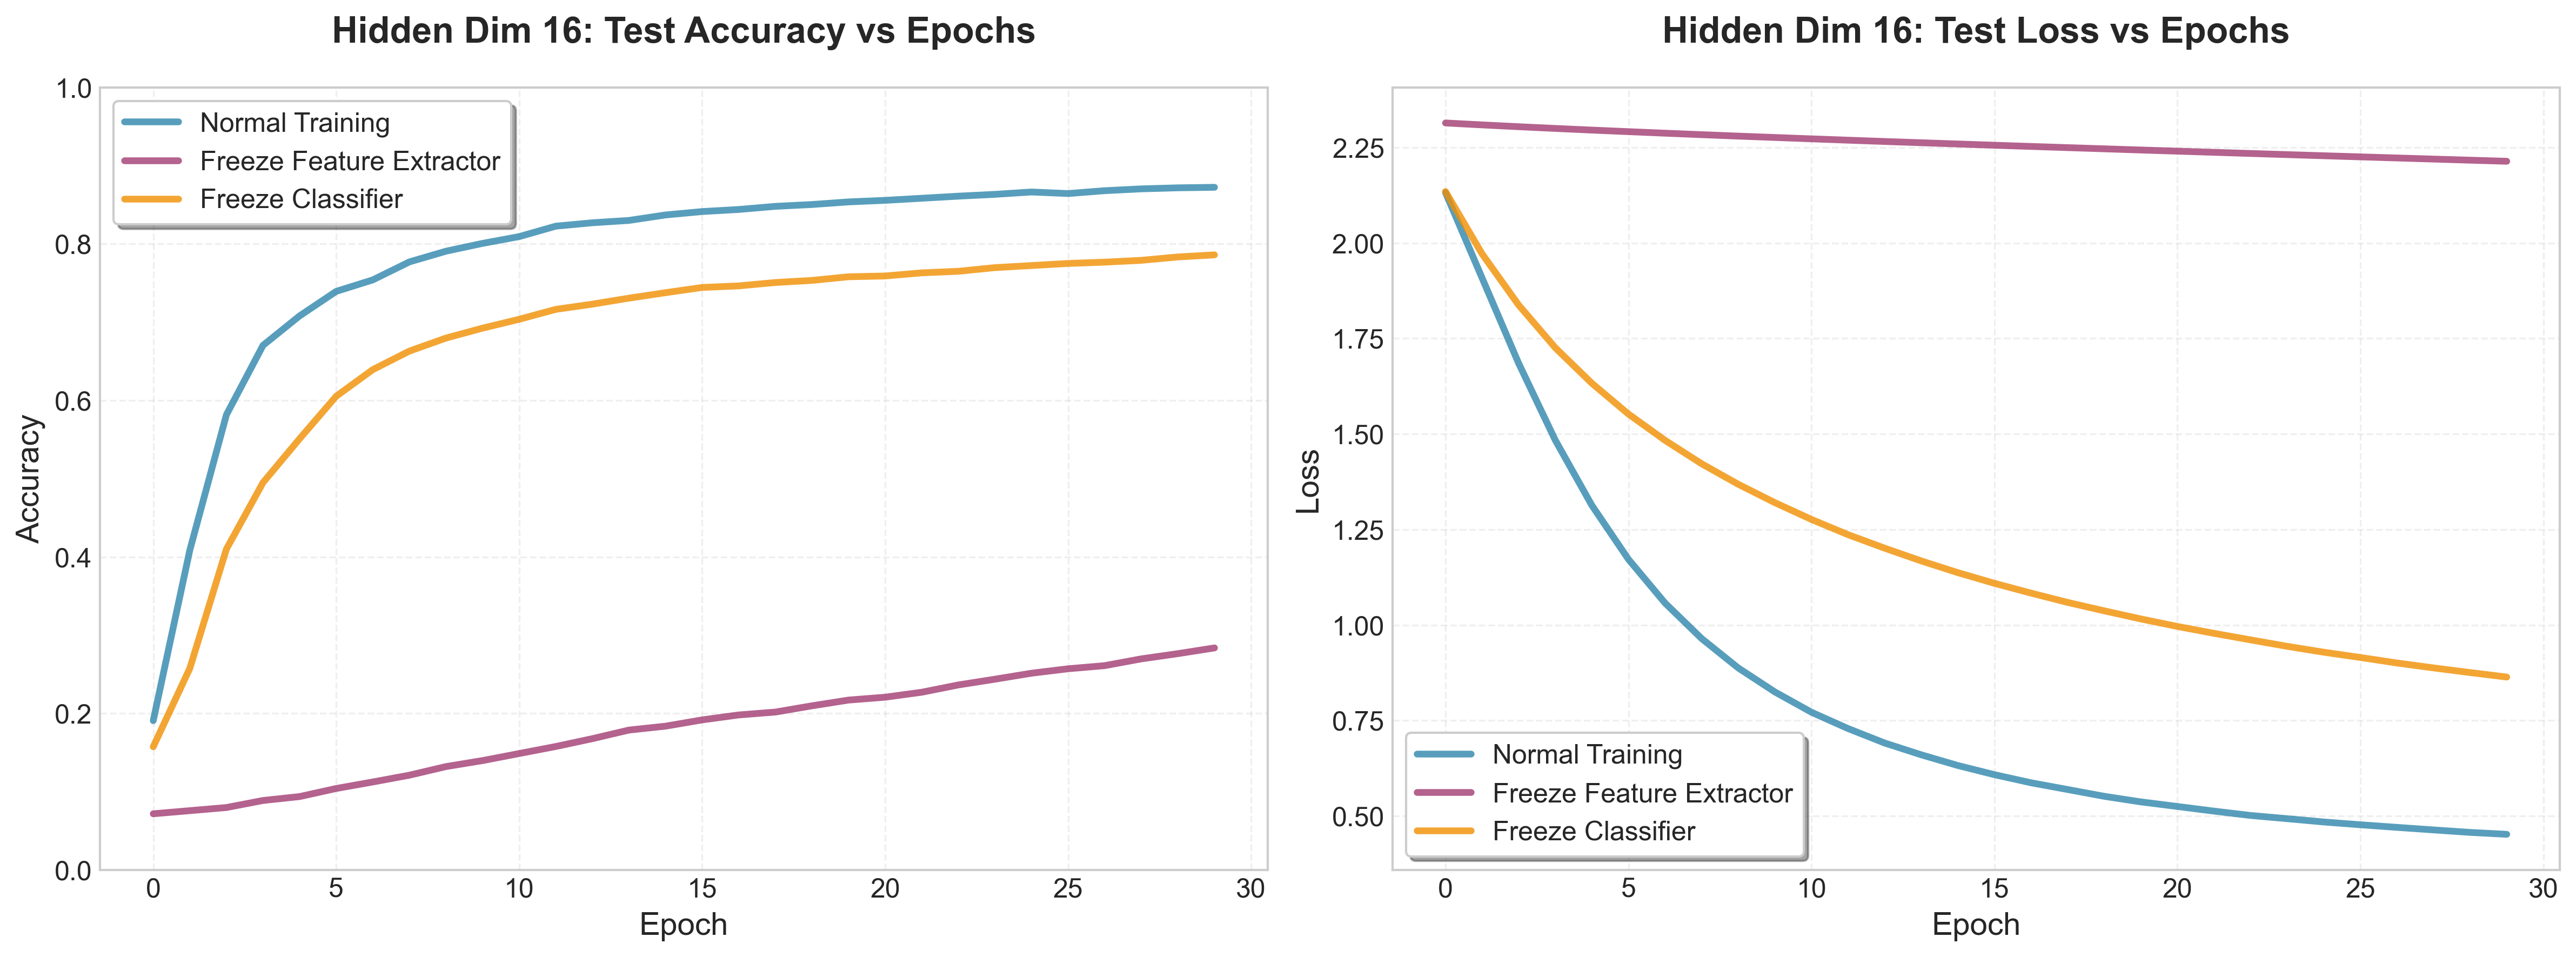
\includegraphics[width=0.8\textwidth]{../images/dd/hidden_16_comparison.png}
    \caption{冻结实验结果对比(隐藏层神经元数为16)}
    \label{fig:hidden_16_comparison.png}
\end{figure}
\begin{figure}[H]
    \centering
    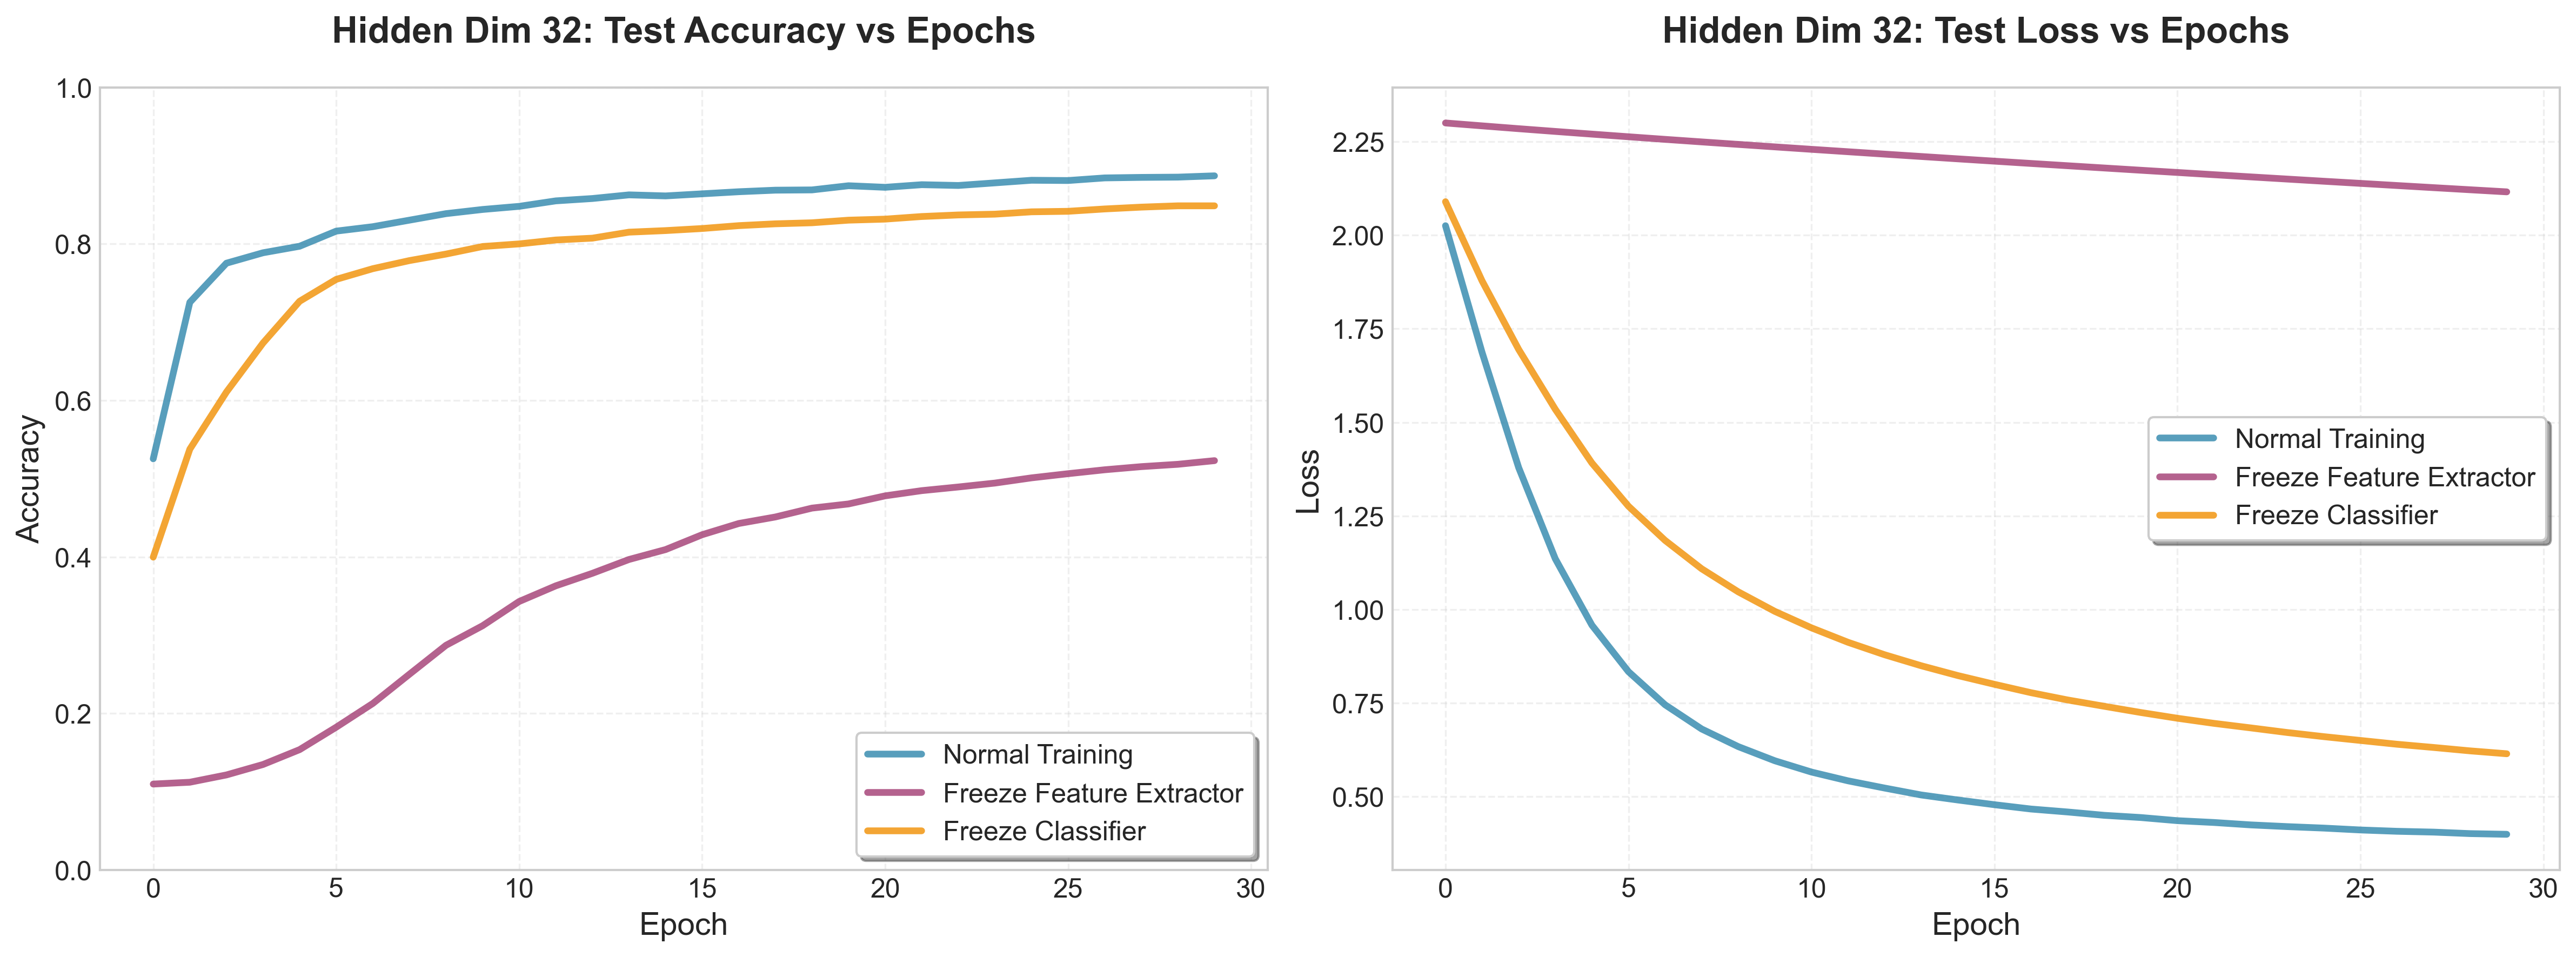
\includegraphics[width=0.8\textwidth]{../images/dd/hidden_32_comparison.png}
    \caption{冻结实验结果对比(隐藏层神经元数为32)}
    \label{fig:hidden_32_comparison.png}
\end{figure}
\begin{figure}[H]
    \centering
    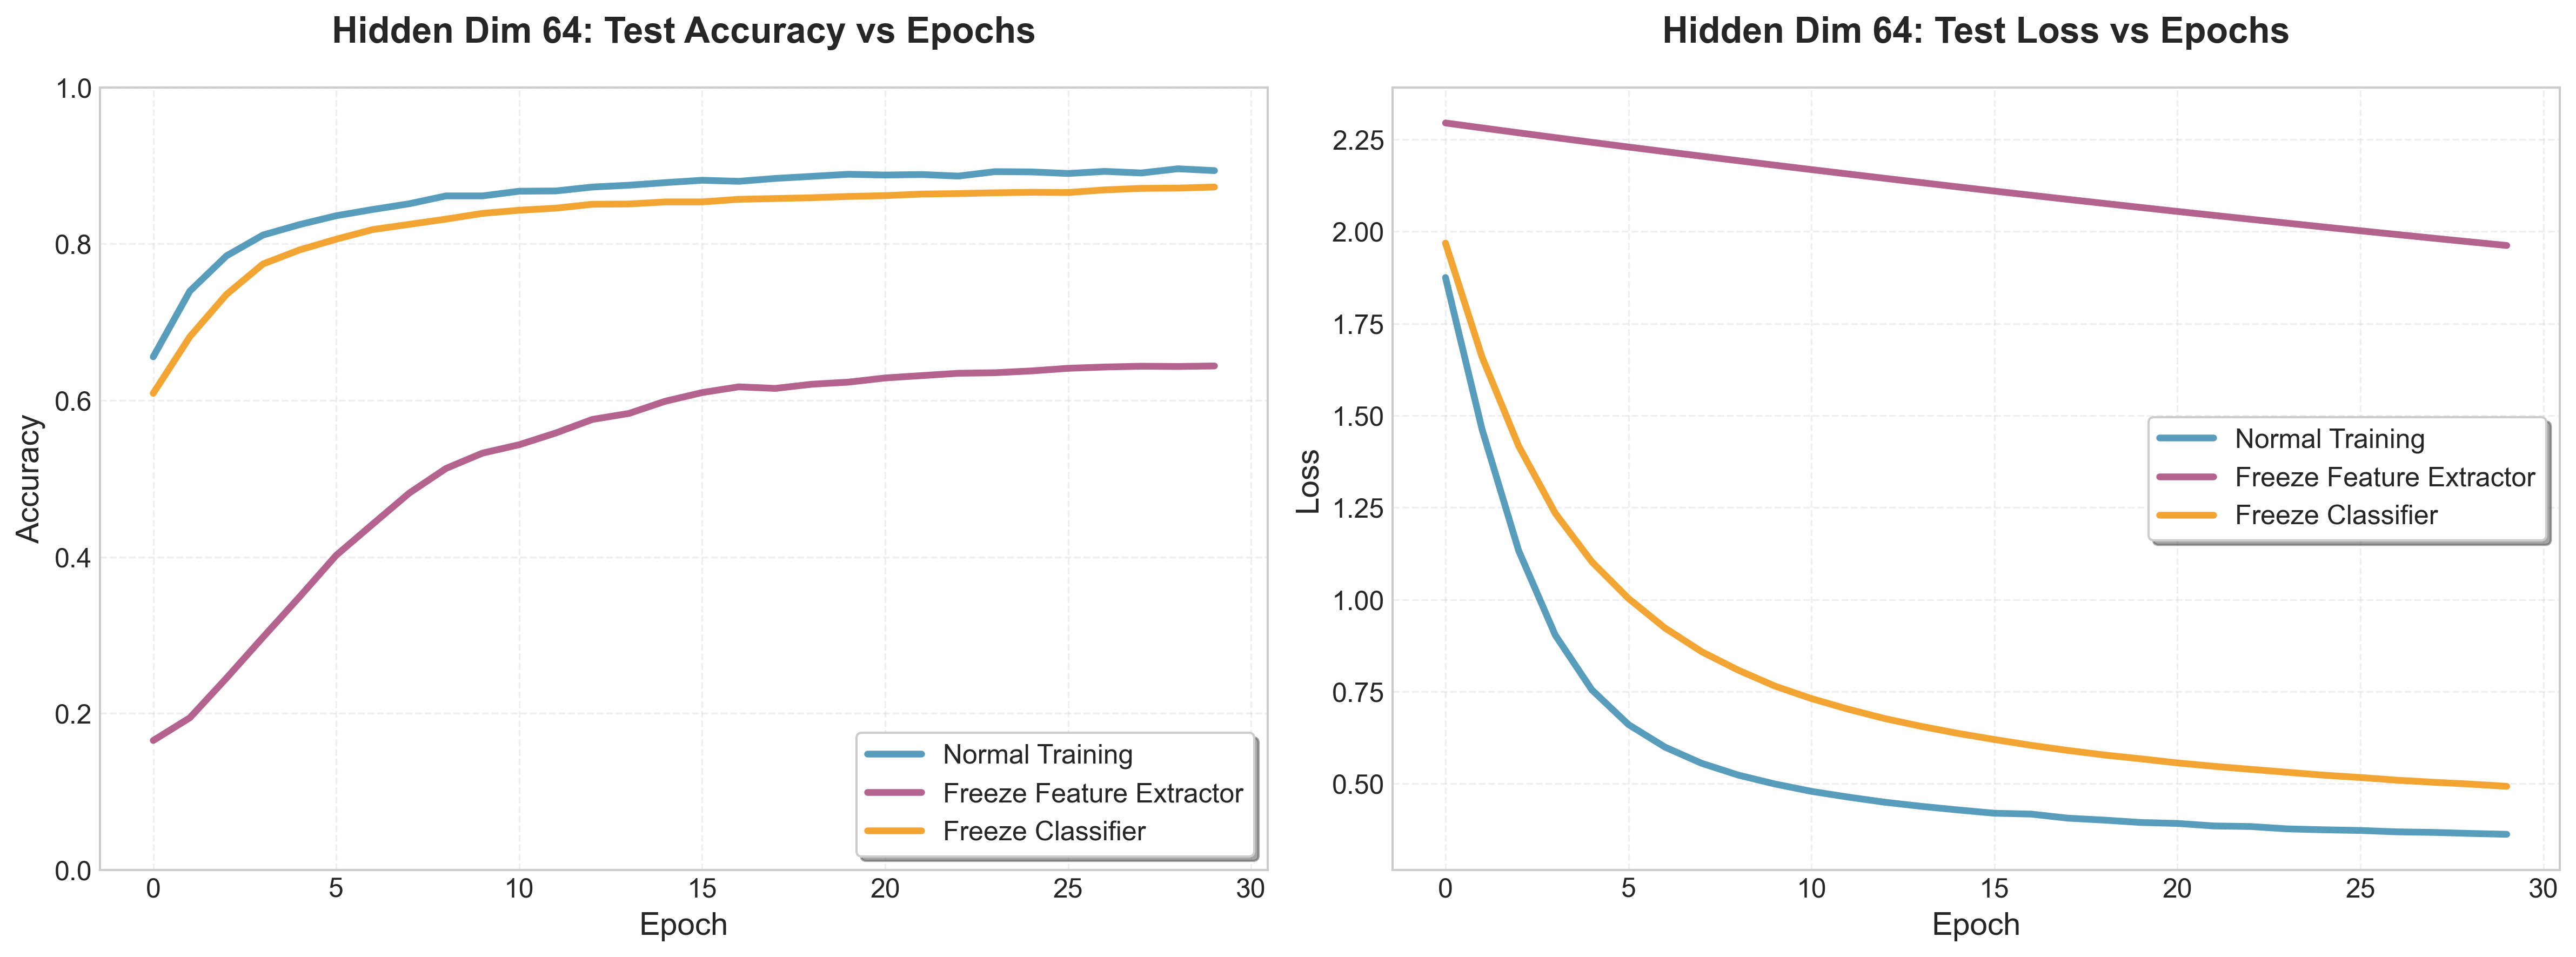
\includegraphics[width=0.8\textwidth]{../images/dd/hidden_64_comparison.png}
    \caption{冻结实验结果对比(隐藏层神经元数为64)}
    \label{fig:hidden_64_comparison.png}
\end{figure}
\begin{figure}[H]
    \centering
    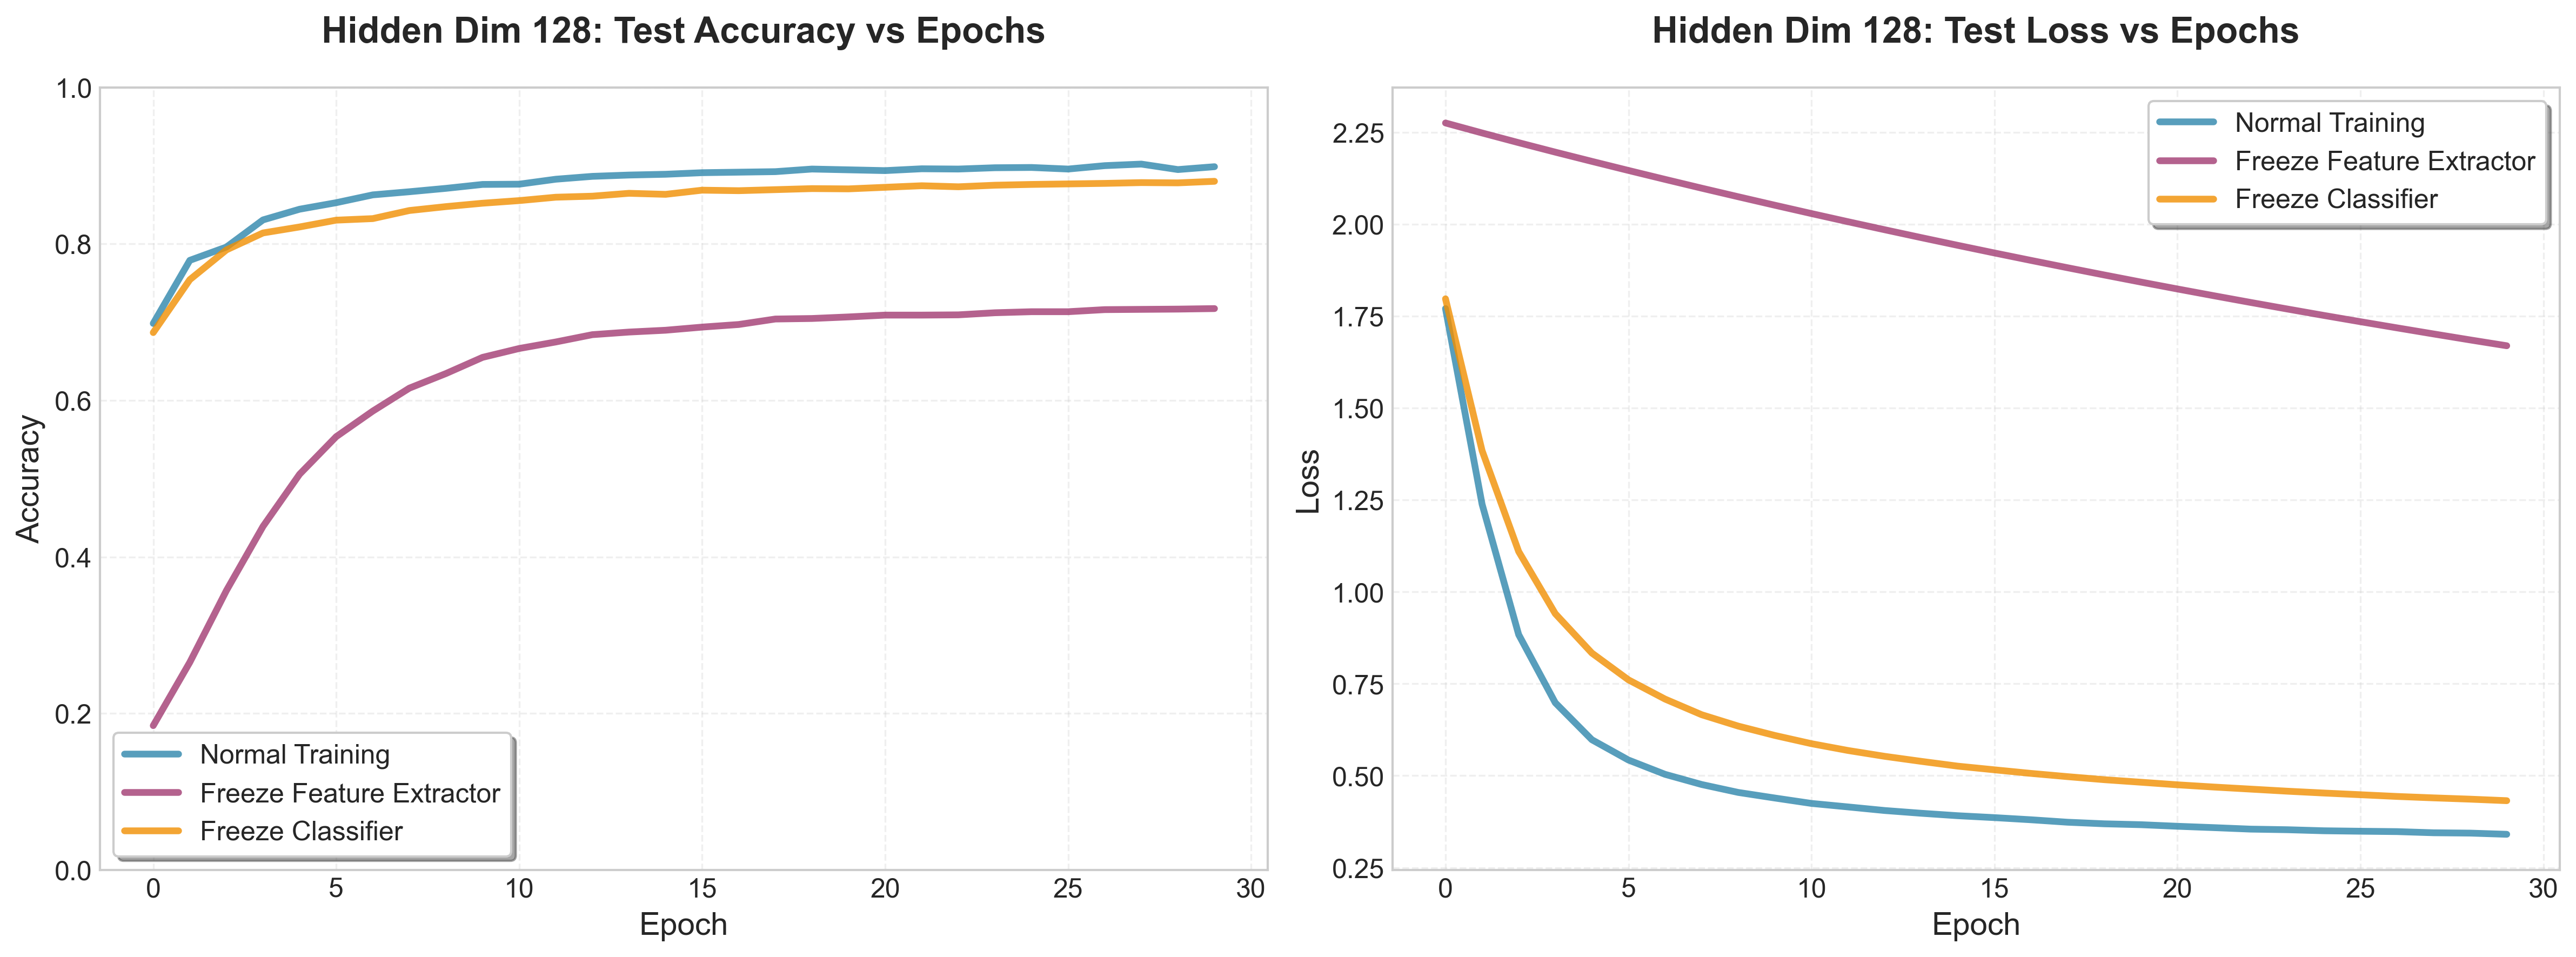
\includegraphics[width=0.8\textwidth]{../images/dd/hidden_128_comparison.png}
    \caption{冻结实验结果对比(隐藏层神经元数为128)}
    \label{fig:hidden_128_comparison.png}
\end{figure}
\begin{figure}[H]
    \centering
    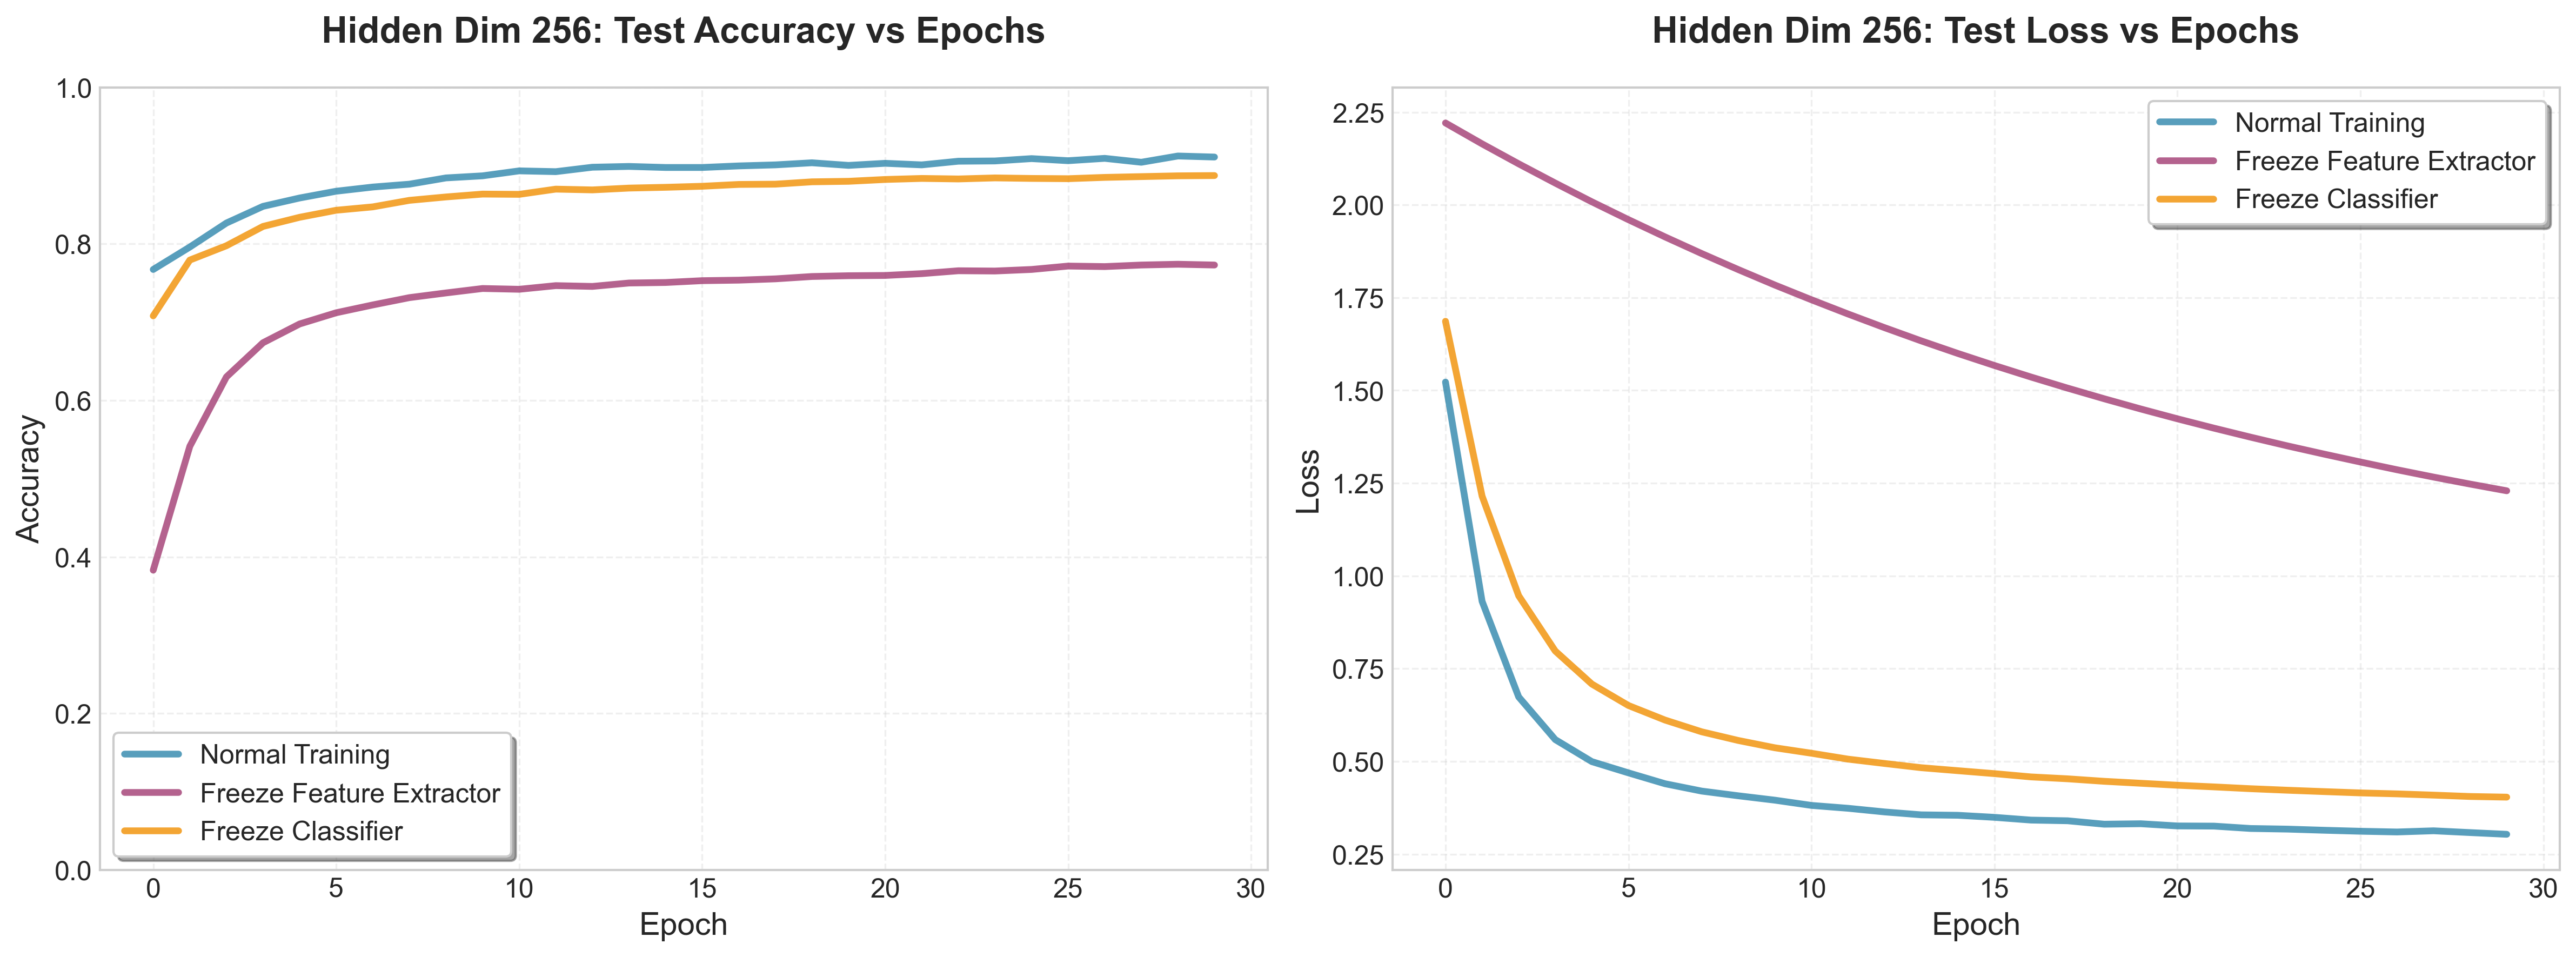
\includegraphics[width=0.8\textwidth]{../images/dd/hidden_256_comparison.png}
    \caption{冻结实验结果对比(隐藏层神经元数为256)}
    \label{fig:hidden_256_comparison.png}
\end{figure}


\section{团队分工}

本项目由五位成员共同完成,团队分工明确,协作紧密。具体任务分配如下表所示:

\begin{table}[H]
  \centering
  \caption{团队成员分工表}
  \begin{tabular}{cll}
    \toprule
    姓名 & 主要负责内容  \\\midrule
    张子路 & 实验任务设计,实验报告撰写 \\\
    郭子逸 & 手动反向传播实现、MLP/CNN结构设计  \\\
    龚正硕 & 训练曲线绘图 , MNIST统计特征提取 \\\
    康琪 & 实验报告撰写 ,数据处理与可视化分析 \\\
    魏玉涛 & 开发可视化交互组件,t-SNE 降维可视化\\\bottomrule
  \end{tabular}
  \label{tab:team-work}
\end{table}

团队成员在本项目中均积极参与,协作高效,在模型构建、实验验证、现象分析和撰写总结等方面密切配合,确保了项目的完

\end{document}